\documentclass[a4paper,12pt,oneside]{book}
\usepackage[utf8]{inputenc}
\usepackage{graphicx}
% \graphicspath{{./pics/}}
\usepackage{amsmath,amsthm,amssymb,amsfonts}
\usepackage{tikz}
\usepackage{pgfplots}
\usetikzlibrary{patterns} 
\usetikzlibrary{shadings}
\usetikzlibrary{decorations.markings}

\usepackage{hyperref} %生成引用链接,注:该宏包可能与其他宏包冲突,故放在所有引用的宏包之后
\usepackage{cleveref} %实现图片和表格、公式的引用,cleveref包必须放在hyperref包之后

\hypersetup{   %链接设置
hidelinks,
colorlinks=true,
linkcolor=red,
citecolor=blue,
urlcolor = black
}

\usepackage{subfig}  % 画子图
\usepackage[title,titletoc]{appendix}

\begin{document}

\author{Avinash K Dixit}
\title{Optimization in Economic Theory \\  \normalsize{2nd Edition}  }   
\date{July 1990}

\frontmatter
\maketitle
\tableofcontents

\mainmatter
\chapter{Introduction}

Economics has been defined as the study of making the best use of scarce resources, that is, of maximization subject to constraints. The criterion being maximized, and the constraints imposed on the choice, vary from one context to the next: households' consumption and labor supply, firms' production, and governments' policies. But all constrained maximization problem have a common economic intuition for them. This book aims to outline the mathematics and develop the intuition.

The standard model of a consumer's choice provides a good point of departure. The basic concepts are a budget line and a set of indifference curves. The points on the budget line represent all affordable combinations of two goods. The family of indifference curves represents the objective, namely to reach as high a curve as possible. The optimum is where an indifference curve is tangential to the budget line. Figure \ref{Fig1.1} shows the familiar picture.

In this chapter I shall develop this model further, using verbal and geometric arguments, but with an eye toward the mathematical sharpening and generalization that will occupy us in later chapters.

It helps to give a little algebraic content to the various magnitudes in Figure \ref{Fig1.1}. Write $I$ for the consumer's money income, $p_1$ and $p_2$ for the prices of the two goods, and $x_1$ and $x_2$ for their quantities. The budget line, where the expenditure exactly equals income, can then be expressed by the equation

%\begin{figure}[!htb] %H为当前位置,!htb为忽略美学标准,htbp为浮动图形
%\centering %图片居中
%\includegraphics[width=0.8\textwidth]{./Fig1.1.png} %插入图片,[]中设置图片大小,{}中是图片文件名
%\caption{The consumer's optimum choice} %最终文档中希望显示的图片标题
%\label{Fig1.1} %用于文内引用的标签
%\end{figure}


\begin{figure}[!tb] %H为当前位置,!htb为忽略美学标准,htbp为浮动图形
\centering %图片居中
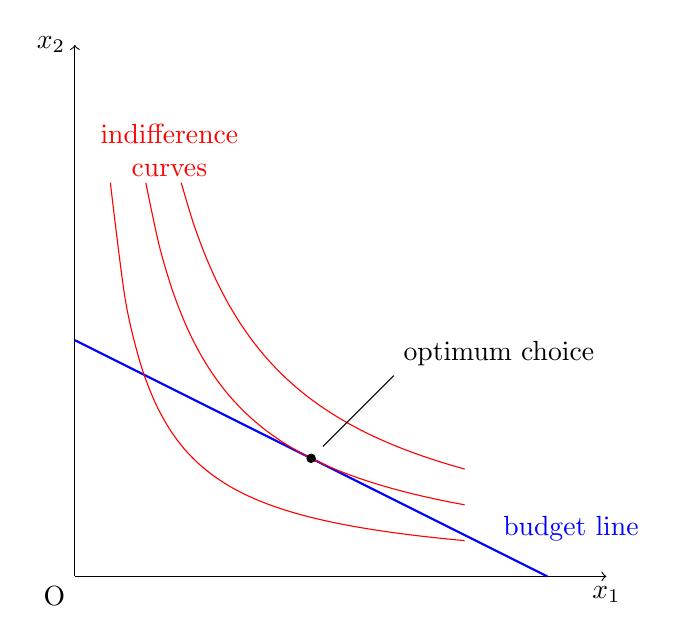
\begin{tikzpicture}[scale=1.5]
    % 绘制坐标轴
    \draw[->] (0,0) -- (4.5,0) node[below] {$x_1$};
    \draw[->] (0,0) -- (0,4.5) node[left] {$x_2$};
    \draw[black] (0,0) node[below left] {O};

% 预算约束线 x1 + 2 x2 = 4
    \draw[thick,blue] (0,2) -- (4,0) ; 
    \draw[thick,blue] (4.2,0.6) node[below] {budget line};

% 无差异曲线 x1 * x2 分别等于1,2,3
    \draw[domain=0.3:3.3,smooth,variable=\x,red] plot ({\x},{1/\x}) ;
    \draw[domain=0.6:3.3,smooth,variable=\x,red] plot ({\x},{2/\x}) ;
    \draw[domain=0.9:3.3,smooth,variable=\x,red] plot ({\x},{3/\x}) ;
    \draw[red] (0.8, 3.3) node[above, align=center] {indifference \\ curves};

% 标记均衡点(假设)
    \filldraw [black] (2,1) circle (1pt) ;
    \draw[black] (2.1, 1.1) -- (2.7,1.7) node[above right] {optimum  choice} ;
\end{tikzpicture}
\caption{The consumer's optimum choice} %最终文档中希望显示的图片标题
\label{Fig1.1} %用于文内引用的标签
\end{figure}


\begin{equation}\label{equa1.1}
p_1 x_1 + p_2 x_2 = I
\end{equation} 

The consumer's preferences over the amounts $x_1$ and $x_2$ of these goods are represented by a numerical scale, called the utility function. This assigns to each bundle $(x_1, x_2)$
of goods a number $U(x_1, x_2)$, called its utility level. In any comparison among alternative bundles, the preferred bundle is the one that receives the highest utility number. Along an indifference curve, all points must have the same utility number. Therefore such a curve has an equation

\begin{equation}\label{equa1.2}
U(x_1, x_2) = \mbox{constant}
\end{equation} 

The exposition of the theory now proceeds by calculating the slopes of the budget line and the indifference curve. For tangency between the two, the slopes must be equal. I shall do this soon. But let me begin with a much simpler and more intuitive approach.

\section*{The Arbitrage Argument}

The idea is to have the consumer start with any trial allocation of his budget, and contemplate a change. If this leads to a bundle of goods that he rates higher on his utility scale, then it is to be adopted as a new trial allocation. Once a bundle is found that cannot be bettered in this way, it will be the optimum allocation, and will be the one actually consumed. Thus the impossibility of finding an improvement will serve as the test of optimality.

The change does not entail any additional expenditures; it is merely a reallocation of some amounts of money from the purchaser of one good to the other. If the initial allocation is not optimal, this can raise the consumer's utility. When the consumer has made the best choice and reached his personal equilibrium, such opportunities for doing better with no net increase in expenditure vanish. This has a close parallel in financial markets. Outside a market equilibrium, participants can make `arbitrage' profits at a zero net outlay, taking advantage of discrepancies in prices of the same asset in different markets. In equilibrium there are no such opportunities. In fact, the very process of people seeking arbitrage profits brings about the equilibrium. I shall exploit this intuitive parallel by labeling this whole line of reasoning the `arbitrage argument', and the resulting optimality condition the `no-arbitrage argument'.

If goods are indivisible, these changes must occur in discrete steps. However, it is often a good approximation to suppose that goods are perfectly divisible. Then the changes can occur in infinitesimal amounts, or what economists call marginal adjustments. Even for seemingly indivisible goods, such as cars or other large consumer durables, there are dimensions of quality etc. that allow continuous adjustment. In any event, such marginal changes are the subject of our analysis in this book.

The standard symbol for `a small (marginal, infinitesimal) change in the variable $x$' is $dx$. This is not to be thought of as the product of two variables $d$ and $x$, but an entity $dx$ in its own right. The use of such infinitesimal magnitudes can be justified rigorously, but for the most part I shall use them in a loose heuristic way. Where you doubt a statement involving infinitesimals, or are unsure I have used them correctly, you should rework the argument using proper calculus methods, starting with a finite change $\Delta x$ and then going to the limit as $\Delta x \rightarrow 0$.

First suppose that initial allocation of the budget has positive amounts $x_1$ and $x_2$ of both goods. Now contemplate a small arbitrage operation, or a marginal reallocation of a small but positive amount of income $dI$ from good 2 to good 1. In physical terms, this means buying $dI/p_1$ units more of good 1 and $dI/p_2$ units less of good 2. Let $MU_1$ and $MU_2$ denote the marginal utilities of the two goods. This means that a small change $dx_1$ in the quantity of good 1 changes utility by $MU_1 dx_1$ units, and similarly $MU_2 dx_2$ for good 2. When the quantities of both goods are changing, the two effects can be added together, so the change in utility is

\begin{equation}\label{equa1.3}
MU_1 dx_1 + MU_2 dx_2
\end{equation} 

In later chapters I shall express this more rigorously using partial derivatives and Taylor series, but the simple statement will suffice here. The important point is that any one marginal adjustment is so small that any changes in the marginal utilities themselves during its course can be neglected. Of course if many such marginal adjustments are strung together, the marginal utilities will change gradually over this sequence. In particular, if $x_2$ rises and/or $x_1$ falls, $MU_2/MU_1$ will fall; this is the principle of the diminishing marginal rate of substitution in consumption. But for the moment I am speaking of just one marginal adjustment. 

The effect of the arbitrage operation on utility is then easy to compute. The increase of $dI/p_1$ in the quantity of good 1 raises utility by $MU_1 dI/p_1$, while the decrease of $dI/p_2$ in the quantity of good 2 lowers utility by $MU_2 dI/p_2$. The net increase in utility is therefore

\begin{equation*}
(MU_1 /p_1 - MU_2 /p_2) dI
\end{equation*} 

If this expression is positive, the consumer will carry out this reallocation and try further reallocation in the same direction. If the initial consumption bundle is optimum, therefore, the expression cannot be positive. This is a part of the `no-arbitrage' criterion of optimality. Since $dI$ was chosen positive, we can divide by it and write the criterion as 

\begin{equation}\label{equa1.4}
(MU_1 /p_1 - MU_2 /p_2) \leq 0
\end{equation} 

Now suppose the criterion is not met, that is, suppose the left-hand side expression in (\ref{equa1.4}) is > 0. Therefore some switch of expenditure toward good 1 is desirable. How far should this process go? Recall that as $x_1$ increases and $x_2$ decreases, $MU_1$ will gradually fall relative to $MU_2$. Eventually a point will be reached where the expression in (\ref{equa1.4}) is zero, and no further move in this direction can raise the consumer's utility level.

Next consider a reallocation in the opposite direction. This will switch the signs in all the above arguments. If the initial allocation is optimum, we must have

\begin{equation}\label{equa1.5}
(MU_1 /p_1 - MU_2 /p_2) \geq 0
\end{equation} 

If this if false, that is, if the expression is < 0, then the process of increasing $x_2$ and decreasing $x_1$ will be carried out until the expression reaches zero.

We can combine the two criteria of optimality of the initial consumption bundle into one: if the allocation $(x_1, x_2)$, with both quantities positive, is optimum, then the marginal utilities at this point must satisfy

\begin{equation}\label{equa1.6}
MU_1 /p_1 = MU_2 /p_2
\end{equation} 

This is the overall `no-arbitrage' condition. The economic interpretation is that at the optimum the consumer should be indifferent between allocating the marginal unit of money to the one good or the other.

\section*{The Tangency Condition Using Calculus}

The more complex but more commonly used way to derive the same condition of optimality is based on the tangency of the budget line (\ref{equa1.1}) and the indifference curve (\ref{equa1.2}). Write the equation of the budget line as 

\begin{equation*}
x_2 = (I/p_2) - x_1 (p_1 / p_2)
\end{equation*} 

Then we see at once that the slope of the line is $(p_1 / p_2)$ in numerical value. The slope of the indifference curve is the marginal rate of substitution(MRS) in consumption, and it equals the ratio of the marginal utilities $(MU_1 / MU_2)$. A heuristic derivation of this is as follows. If a marginal loss of $dx_1$ units of good 1 is just compensated by the marginal gains of $dx_2$ units of good 2, then the marginal rate of substitution(MRS) is the ratio $dx_2 / dx_1$. But the exact offset of the gain can be written as an equation in utility units

\begin{equation*}
MU_1 dx_1 = MU_2 dx_2
\end{equation*} 

Therefore

\begin{equation}\label{equa1.7}
MRS = dx_2 / dx_1 = MU_1 / MU_2
\end{equation} 

Incidentally, note the reversal of the subscripts 1 and 2 between the numerator and the denominator of the two ratios. This is not a typographical error; that is how the ratios are related, as you can see by cross-multiplying to get back to the equation just above.

At the optimum, the slope of the indifference curve (the marginal rate of substitution in consumption) is equal to the slope of the budget line (the price ratio). Therefore

\begin{equation}\label{equa1.8}
MU_1 / MU_2 = p_1 / p_2
\end{equation} 

This is equivalent to the optimality criterion (\ref{equa1.6}) we derived before. However, the verbal argument underlying (\ref{equa1.6}) has some advantages over the geometry of (\ref{equa1.8}). 

\section*{Corner Solutions}

The arbitrage argument is somewhat easier to adapt to the case where one of the goods is not bought at all. Since this occurs at one end or the other of the budget line, such optima are often called corner solutions. Suppose all income is spent on good 2 in the initial allocation, so $x_1 = 0$ and $x_2 = I/p_2$. Now of the two directions of improvement, namely trying to increase $x_1$ and to decrease it, only the former is possible. Therefore only the criterion (\ref{equa1.4}) corresponding to this test survives. Since $x_1$ cannot be decreased any further, the argument leading to (\ref{equa1.5}) cannot be made. The economic interpretation of (\ref{equa1.4}) holding for the consumption bundle $(0, I/p_2)$ is equally simple: even the first little units of income spent on good 1 does not bring enough utility benefit to match that from the last unit spent on good 2.

\section*{Marginal Utility of Income}

The second advantage of the arbitrage argument is even more important. Return to the situation where both goods are initially bought, and the criterion (\ref{equa1.6}) for optimality. Now suppose our consumer is given an extra amount $dI$ of income to spend. He could spend it all on good 1, buy $(dI/ p_1)$ more units of it and achieve an additional $(MU_1 dI/p_1)$ units of utility. Or he could spend it all on good 2, when his utility would increase by $(MU_2 dI / p_2)$ units. But the two increments to utility are equal by (\ref{equa1.6}). Therefore at the margin the allocation of the inifinitesimal amount $dI$ of extra income to good 1, or good 2, or indeed any mixture of the two, is a matter of indifference to the consumer. Then we can call the utility increment per unit of marginal addition to income simply the marginal utility of income, without bothering to specify how the marginal addition to the income is spent. Write $\lambda$ for this marginal utility of income. Then the $dI$ units of extra income raise utility by $\lambda dI$ units. Equating this to the two other ways of writing the same utility gain in terms of spending on each of the two goods, we find

\begin{equation}\label{equa1.9}
\lambda = MU_1 / p_1 = MU_2 / p_2
\end{equation} 

We see that the common value of the two sides in the optimality criterion (\ref{equa1.6}) has a very useful economic interpretation -- it is the marginal utility of income. A very similar interpretation is possible for the no-arbitrage conditions in all constrained optimization problems; I shall explain this in greater detail and unify it under the concept of Lagrange multipliers or shadow prices.

\section*{Many Goods and Constraints}

The generalization of the analysis to cover cases where there are several goods, some of which may not be bought at all, is equally easy. Suppose there are $n$ goods, with prices $(p_1, p_2, \dots, p_n$ and quantities $(x_1, x_2, \dots, x_n)$. For all goods bought in positive amounts at the optimum, the ratio of marginal utility to price must have a common value, which can then be interpreted as the marginal utility of income $\lambda$. For all goods not bought, the ratio of marginal utility to price must be smaller than, or at best equals to, this value. In symbols, for any goods $i$,

\begin{equation*}
MU_i / p_i \left\{  \begin{array}{lll}
=\lambda & \mbox{if} & x_i > 0 \\
\leq \lambda & \mbox{if} & x_i=0
\end{array}
\right.
\end{equation*} 

or

\begin{equation} \label{equa1.10}
MU_i - \lambda p_i \left\{  \begin{array}{lll}
=0 & \mbox{if} & x_i > 0 \\
\leq 0 & \mbox{if} & x_i=0
\end{array}
\right.
\end{equation} 

The method can also be extended to allow several constraints. We need a separate $\lambda$ for each constraints, and it can be interpreted as the marginal utility of relaxing that constraint. I shall discuss this in Chapter 3.

\section*{Non-binding Constraints}

Finally, consider an extension that is not of great relevance in consumer theory, but will prove very important in some other applications. Picture a consumer with an income so large that he is satiated, and fails to spend it all. The budget equation (\ref{equa1.1}) should be replaced by an inequality

\begin{equation*}
p_1 x_1 + p_2 x_2 \leq I
\end{equation*} 

We can bring this within the scope of the above theory simply by defining a new good $x_3$, `unspent income', which has price equal to one and yield no utility. (Note that I am not talking of saving, which enables a non-satiated consumer to spend more on desired goods in the future, but of totally useless unspent income.) The budget equation becomes

\begin{equation*}
p_1 x_1 + p_2 x_2 + x_3 = I
\end{equation*} 
and we have $MU_3 \equiv 0$. Since we are supposing that the consumer is choosing a positive amount of $x_3$, (\ref{equa1.10}) for $i=3$ gives $\lambda=0$. This makes intuition sense: if the consumer does not even spend all the income he has, then the marginal utility of an increment to income should be zero. In turn, we can use this in (\ref{equa1.10}) corresponding to the other goods, and obtain $MU_i =0$ for $i=1$ and 2. Thus these goods are consumed at a level that yields zero marginal utility, that is, to the point of satiation.

We started on a simple and intuitive excursion into a consumer's choice problem, using nothing but the computation of `arbitrage' gains and losses from marginal adjustments and building them into criteria of optimality. This has already brought us to a very important general way of characterizing optima subject to constraints. In fact (\ref{equa1.10}) is nothing but a form of a basic result of the theory of optimization subject to constraints, namely the Kuhn-Tucker Theorem. The extension to the case of a satiated consumer is an instance of the general principle known as Complementary Slackness. In the chapters that follow, I shall gradually develop the general theory in a more systematic way, making use of the calculus, to develop and to sharpen the intuitive ideas introduced here.


\chapter{Lagrange’s Method}

\section*{Statement of the Problem}

Let us begin the development of the general theory of optimization subject to constraints, using a setting very close to the consumer choice model of Chapter 1. Suppose the choice variables are $x_1$ and $x_2$. I shall write them more compactly as a vector $x$ arranged in a column,

\begin{equation*}
   x = \left( \begin{array}{c}
   x_1 \\
   x_2
   \end{array}
   \right)
\end{equation*}
Initially, I shall use vectors only to abbreviate lists of components; actual operations with vectors and matrices will appear gradually.

We will need notation that distinguishes between the general vector $x$ and some particular value of $x$ such as the optimum, while remembering the family resemblance between the two: both are vectors of choice variables. I shall generally use the symbol $\bar{x}$ to denote the optimum value of the general variable $x$. The components of $\bar{x}$ will be written $\bar{x}_1$ etc.

The function to be maximized, called the objective function, is $F(x)$. The constraint is a general non-linear one,

\begin{equation}\label{equa2.1}
G(x)=c
\end{equation}
where $G$ is a function and $c$ a given constraint. The model of Chapter 1 was a special case of this: $F$ was the utility function, $G$ was a linear function showing the expenditure,
\begin{equation*}
G(x) = p_1 x_1 + p_2 x_2
\end{equation*}
and $c$ was income. If it helps, you can now think of $G$ as a more general non-linear expenditure or cost function, such as would arise if the consumer faced a quantity discount or premium price schedule.

With this notation, the problem in this chapter is to find the value $\bar{x}$ that maximizes $F(x)$ subject to $G(x)=c$.

\section*{The Arbitrage Argument}

As we did in Chapter 1, start with a trial point and an infinitesimal change. Let the particular trial point be $\bar{x}$, and the infinitesimal change
\begin{equation*}
 dx = \left(
 \begin{array}{c}
 dx_1 \\ dx_2
 \end{array}
 \right)
\end{equation*}
We want $(\bar{x} + dx)$ to satisfy the constrain, and see if it yields a higher value of the objective function.

Since the change in $x$ is infinitesimal, we can approximate the changes in values in functions of $x$ by the first-order linear terms in their Taylor series. Let subscripts on a function denote its partial derivatives with respect to the indicated argument; for example $F_1$ is $\partial F/ \partial x_1$. We must remember that in general each partial derivative is itself a function of the whole vector $x$. Only in the special case where $F$ is linear will the partial derivatives be constraints; only in the special case where $F$ is additivity separable (a function of $x_1$ plus a function of $x_2$) will $F_1$ be independent of $x_2$ and vice versa. Thus we should write the partial derivatives as function $F_1(x)$ and $F_2(x)$. When these are evaluated at our initial trial point $\bar{x}$, their values will be written $F_1(\bar{x})$ and $F_2(\bar{x})$.

The first-order Taylor approximation of the change in $F(x)$ as a result of the infinitesimal move from the general point $x$ to $x+dx$ is
\begin{equation}\label{equa2.2}
  \begin{array}{rl}
dF(x) & = F(x+dx)-F(x) \\
      & = F_1(x) dx_1 + F_2(x) dx_2
  \end{array}
\end{equation}
Observe the similarity with the expression for the change in utility (\ref{equa1.3}) of Chapter 1; the marginal utilities that were motivated there by economic intuition are simply the partial derivatives of the utility function with respect to the amounts of the two goods consumed.

There is a similar expression for the change in $G(x)$:
\begin{equation}\label{equa2.3}
dG(x) = G_1(x) dx_1 + G_2(x) dx_2
\end{equation}
In Chapter 1, the partial derivatives of $G$ were simply the prices. If we now think of $G$ as a more general non-linear outlay or expenditure function, the partial derivatives are the marginal prices of the respective commodities.

Now we can modify the arbitrage argument of Chapter 1 to apply to the new more general setting. Start at a point $\bar{x}$ where the constraint (\ref{equa2.1}) holds, and consider a change $dx$ such that $(\bar{x}+ dx)$ also satisfies the constraint. Then $dG(\bar{x})=0$. Using (\ref{equa2.3}) with the particular initial point, we have
\begin{equation*}
G_1(\bar{x}) dx_1 = - G_2(\bar{x}) dx_2
\end{equation*}
Call the common value of these two sides $dc$. Then our arbitrage consists of reallocating an amount $dc$ in the value of the function $G(x)$ away from $x_2$ and toward $x_1$.

First Suppose $G_1(\bar{x})$ and $G_2(\bar{x})$ are both non-zero. Then\begin{equation*}
dx_1 = dc / G_1(x)  \mbox{\quad and \quad}   dx_2 = dc / G_2(x)
\end{equation*}
The resulting change in the value of the objective function is found by substituting into (\ref{equa2.2}) as
\begin{equation}\label{equa2.4}
dF(\bar{x}) = [F_1(\bar{x}) / G_1(\bar{x})  - F_2(\bar{x}) / G_2(\bar{x})  ] dc
\end{equation}

If the bracketed expression is non-zero, then $F(x)$ can be increased by choosing $dc$ to have the same sign as that of the bracketed expression. As before, we can turn this around to find a no-arbitrage condition that holds when $\bar{x}$ is the optimum choice. So long as neither $\bar{x}_1$ nor $\bar{x}_2$ has hit some natural boundary such as zero, then changes $dc$ of either sign are possible. If $\bar{x}$ is optimum, then no such change should be capable of increasing $F(x)$. Therefore the bracketed expression in (\ref{equa2.4}) should be zero, or
\begin{equation}\label{equa2.5}
F_1(\bar{x}) / G_1(\bar{x})  = F_2(\bar{x}) / G_2(\bar{x})
\end{equation}
This is the analog of the condition (\ref{equa1.6}) of the previous chapter.

Note the exact statement: $if$ the optimum choice is $\bar{x}$, $then$ it satisfies (\ref{equa2.5}). I have not established any implication the other way round, so there is no guarantee that a solution to (\ref{equa2.5}) is the optimum. This is the difference between necessary and sufficient conditions, and I will discuss it in more detail later in this chapter.

If $\bar{x}$ lies at some natural boundary, for example if one of $\bar{x}_1$ and $\bar{x}_2$ is zero when both must be non-negative, then only one-sided changes $dc$ are meaningful, and we get an inequality that corresponds to (\ref{equa1.4}) and (\ref{equa1.5}). I shall not consider this case in this chapter, but shall return to it in the next.

As in Chapter 1, let us define $\lambda$ to be the common value of the two sides in (\ref{equa2.5}). Then we can write that equation as a set of two equations
\begin{equation}\label{equa2.6}
F_j(\bar{x}) = \lambda G_j(\bar{x}), \mbox{\quad} j=1,2
\end{equation}
Remember that the $\lambda$ of Chapter 1 could be interpreted as the marginal utility of income. In the same way, the $lambda$ just introduced turns out to be the rate at which the optimum value of $F(x)$ responds to a change in $c$. I shall develop this interpretation and its implications in Chapter 4. The main topic in the rest of this chapter involves writing \ref{equa2.6}) in a way that easily extends to more general settings, and provides a method for finding the optimum $x$. But first a couple of necessary digressions.

\section*{Constraint Qualification}

What happens if say $G_1(\bar{x})$ is zero? Now $bar{x}_1$ can be changed slightly without affecting the constraint. If $F_1(\bar{x})$ is not zero, it is desirable to do so. For example, if $F_1(\bar{x})$ is positive, then $F(x)$ can be increased by raising $x_1$. This goes on until either $F_1(x)$ drops to zero, or $G_1(x)$ becomes non-zero. In the consumption interpretation, a consumer will go on using more of a free good either until he is satiated, or until the marginal unit of a free good is no longer free. Therefore if $G_1(\bar{x})$ is zero and $\bar{x}$ is optimum, then $F_1(\bar{x})$ must be zero, too. We can define the ratio of these two zeros as we please, and there is no harm in defining it so that (\ref{equa2.5}) is satisfied.

What if $G_1(\bar{x})$ and $G_2(\bar{x})$ are both zero? This might mean that both goods are free, and should be consumed to the point of satiation. But there is a more ominous possibility arising from the quirks of algebra and calculus. Take the budget line (\ref{equa1.1}) of the previous chapter, and write its equation as
\begin{equation*}
(p_1 x_1 + p_2 x_2 -I)^3 = 0
\end{equation*}
This is an unnecessarily complicated way of writing (\ref{equa1.1}), but the two are mathematically fully equivalent, and we should see if the change makes any difference. Let $G(x)$ be the function on the left-hand side of this. Then
\begin{equation*}
G_1(x) = 3 p_1 (p_1 x_1 + p_2 x_2 -I)^2
\end{equation*}
which is always zero when $x$ satisfies the budget constraint. The same is true for $G_2(x)$. Goods are not free at the margin, and yet their quantities have zero effect on the constraint function. In such a case, our method runs into trouble.

The formal mathematical theory cops out and simply refuses to deal with such cases by assuming a condition called a Constraint Qualification. In the present instance that simply amounts to assuming that at least one of $G_1(\bar{x})$ and $G_2(\bar{x})$ is non-zero. If this is not true in a particular application, then conditions like (\ref{equa2.6}) may be invalid there. Luckily, failure of the Constraint Qualification is rarely a problem in practice. In the rara cases where it arises, it can usually be circumvented by writing the algebraic from of the constraint differently, as with the budget constraint above. But students of the subject should not forget the problem altogether; it is a favorite source of trick questions in examinations. If something strange seems to be going wrong when you try the standard methods, you should check to see if the problem violates the Constraint Qualification. But I shall omit further mention of this complication except in the formal statements and mathematical proofs.

\section*{The Tangency Argument}

The second digressions relates the arbitrage argument to the tangency condition more familiar from elementary economic texts. In Chapter 1 we saw an alternative way to obtain the condition (\ref{equa1.6}), based on the tangency of the budget line and an indifference curve. The same can be done for (\ref{equa2.5}). Figure \ref{Fig2.1} shows the story. Along the curve $G(x)=c$, we have $dG(x)=0$, and from (\ref{equa2.3}) we can calculate the slope of the tangent to the curve at $x$ as
\begin{equation}\label{equa2.7}
dx_2 / dx_1 = - G_1(x) / G_2(x)
\end{equation}
\begin{figure}[!tb] %H为当前位置,!htb为忽略美学标准,htbp为浮动图形
\centering %图片居中
%\includegraphics[width=0.8\textwidth]{./Fig2.1.png} %插入图片,[]中设置图片大小,{}中是图片文件名
\begin{tikzpicture}[scale=2]
    % 绘制坐标轴
    \draw[->] (0,0) -- (2.5,0) node[below] {$x_1$};
    \draw[->] (0,0) -- (0,2.5) node[left] {$x_2$};
    \draw[black] (0,0) node[below left] {O};

    \draw[thick,blue] (0.3,1.7) -- (1.7,0.3) ; 
    \draw[thick,blue] (2.8,0) node[above] {common tangent};

% 无差异曲线 x1 * x2 分别等于1,2,3
    \draw[domain=0.5:1.8,smooth,variable=\x,red] plot ({\x},{1/\x}) ;
    \draw[red] (0.8, 2.0) node[above, align=center] {$F(x)=v$};
    
    \draw[domain=0.3:1.4,smooth,variable=\x,red] plot ({\x},{1/(\x-2)+2}) ;
    \draw[red] (0.3, 0) node[above right, align=center] {$G(x)=c$};
    

% 标记均衡点(假设)
    \filldraw [black] (1,1) circle (1pt) node[above right] {$\bar{x}$} ;
    
\end{tikzpicture}
\caption{The tangency solution} %最终文档中希望显示的图片标题
\label{Fig2.1} %用于文内引用的标签
\end{figure}
Note the reversal of the subscripts, exactly as in Chapter 1. Note also that if $G_2(x)=0$ the curve is vertical; this is not a serious problem. If both $G_1(x)$ and $G_2(x)$ are zero, the slope is not well defined, and the method may run into a problem as was explained just above. In most economic applications, $G$ is an increasing function of both arguments. Then $G_1(x)$ and $G_2(x)$ are both positive, $dx_2 /dx_1$ along the curve is negative, and we have the usual downward-sloping transformation frontier for the constraint.

A contour of the objective function $F$, that is, a curve of equal values $F(x)$, runs through the point $x$. The slope of the tangent to the contour at this point is similarly calculated
\begin{equation}\label{equa2.8}
dx_2 / dx_1 = - F_1(x) / F_2(x)
\end{equation}
Once again, in most economic applications, $F$ is an increasing function and the contour (indifference curve) is downward-sloping.

If $\bar{x}$ is optimum, the two curves must be mutually tangential, that is, have the same slope, at this point. Equating the two expressions, we have
\begin{equation}\label{equa2.9}
F_1(\bar{x}) / F_2(\bar{x}) = G_1(\bar{x}) / G_2(\bar{x})
\end{equation}
which is equivalent to (\ref{equa2.5}).

\section*{Necessary vs. Sufficient Conditions}

Recall what the above argument established: $if$ $\bar{x}$ maximizes $F(x)$ subject to $G(x)=c$, $then$ (\ref{equa2.5}) holds. In other words, the condition (\ref{equa2.5}) is a logical consequence of the optimality of $barP{x}$. Therefore it is called a necessary condition for optimality. To be more precise, since it involves the first-order derivatives of the functions $F$ and $G$, it is called the $first-order \ necessary \ condition$.

In searching for an optimum, the first-order necessary condition helps to narrow down the search. The necessary conditions were established starting with an assumed known optimum $\bar{x}$. But we turn the story around by treating the components $\bar{x}_1$ and $\bar{x}_2$ as unknowns, and the constraint (\ref{equa2.1}) and the necessary condition (\ref{equa2.5}) as two equations that will determine them. Typically, there is a whole continuous range of values of $\bar{x}$ satisfying the constraint (\ref{equa2.1}). But there are only a few values of $\bar{x}$, and if we are lucky, just one, that also satisfies the condition (\ref{equa2.5}).

If we know from separate reasoning that our problem indeed has a solution, and we find that there is a unique $\bar{x}$ satisfying the constraint and the first-order necessary condition, then it must be the solution we seek. If there are multiple solutions to (\ref{equa2.1}) and (\ref{equa2.5}) taken together, then all are candidates for optimality as far as the present analysis is concerned, and some other method must be used to find the correct solution. Even then, the first-order necessary condition (\ref{equa2.5}) will have cut down quite drastically the number of candidate points we need to examine.

The main reason that the first-order necessary condition does not always lead us to the right solution is that the same first-order condition is also necessary for the problem of $minimizing$ the same function $F(x)$ subject to the same constraint $G(x)=c$. Minimizing $F(x)$ is the same as maximizing $-F(x)$. By the same reasoning as that leading to (\ref{equa2.8}), we can find the slope of a contour of this function:
\begin{equation*}
dx_2 / dx_1 = - [ -F_1(x)] /[ -F_2(x) ] = - F_1(x) / F_2(x)
\end{equation*}
Equating the value of this at $\bar{x}$ to (\ref{equa2.7}), we get (\ref{equa2.9}) again.

There is also the point that to obtain the condition, we asked if the value $F(x)$ could be improved by making $small$ changes in $x$. If not, then $x$ is better than the comparison points in a small neighborhood, or it yields a local peak of $F(x)$. Now a function can in general have several such local peaks, and several local troughs too. The same first order necessary condition will be true at all these points. Only one will give a true or global maximum.

Finally, either a maximum or minimum implies (\ref{equa2.5}) but not vice versa. Therefore the condition might be satisfied at a point that is neither a maximum nor a minimum, even in a small neighborhood. As a simple example, consider $F(x)= x^3$ where  $x$ is a scalar. We have $F^\prime(0) = 0$, but $x=0$ gives neither a maximum nor a minimum of $F(x)$.

To distinguish such cases, any point satisfying the first order necessary conditions is called a $stationary \ point$. The true optimum is one of the stationary points. To locate it among these candidates, we need some other test. Such tests typically rely on the curvature, or the second-order derivatives, of the functions. In Figure \ref{Fig2.1} the curvatures of the contours of $F$ and $G$ have been chosen correctly for a maximum. Thus the curve $G(x)=c$ gets flatter as $x_1$ decreases and $x_2$ increases along it; the economic interpretation is that the marginal rate of transformation of $x_1$ into $x_2$ diminishes as more and more of such a transformation is carried out. Similarly, the contour of $F$ shows a diminishing marginal rate of substitution.

Test involving curvatures or second-order derivatives are the subject of Chapter 6-8. These tests differ from the first-order conditions of this chapter in another way: $if$ such a condition holds, $then$ the point in question is a maximum, at least in comparison with neighboring points; the condition ensures optimality. Therefore such a condition is called a $second-order \ sufficient$ condition.

\section*{Lagrange's Method}

Now let us express the first-order necessary condition (\ref{equa2.6}) in a way that is easy to remember and use. This is called Lagrange's Method after its inventor. Note that we want to use the condition to solve for the optimum $\bar{x}$. We introduced $\lambda$ as the common value of the two sides in (\ref{equa2.5}), so it is just as much unknown as the optimum $\bar{x}$. That is, we have to determine it as an integral part of the solution. In the meantime, call it an undetermined Lagrange multiplier. Define a new function, called the Lagrangian,
\begin{equation} \label{equa2.10}
L(x, \lambda) = F(x) + \lambda[c - G(x) ]
\end{equation}
Note that $L$ is also a function of $c$, and of any other parameters that appear in the functional forms of $F$ and $G$. Such arguments of $L$ will be shown explicitly only when they are important in the context.

Denote the partial derivatives of $L$ by 
\begin{equation*}
L_j \equiv \partial L/ \partial x_j, \quad L_\lambda \equiv \partial L / \partial \lambda
\end{equation*}
Then
\begin{equation*}
L_j(x, \lambda) = F_j(x) - \lambda G_j(x)
\end{equation*}
and
\begin{equation*}
L_\lambda(x, \lambda) = c- G(x)
\end{equation*}
The first-order necessary condition (\ref{equa2.6}) becomes just $L_j =0$ for $j=1$ and 2, and the constraint (\ref{equa2.1}) simply $L_\lambda =0$. Then we can state the result of the whole argument so far into a simple statement:

$Lagrange's Theorem:$ Suppose $x$ is a two-dimensional vector, $c$ is a scalar, and $F$ and $G$ functions taking scalar values. Define the function $L$ as in (\ref{equa2.10}). If $\bar{x}$ maximizes $F(x)$ subject to $G(x)=c$, with no other constraints (such as non-negativity), and if $G_j(\bar{x}) \neq 0$ for at least one $j$, then there is a value of $\lambda$ such that

\begin{equation} \label{equa2.11}
L_j(\bar{x}, \lambda) = 0  \  for  \ j=1,2  \quad L_\lambda(\bar{x}, \lambda) = 0
\end{equation}

Remember that the theorem provides necessary conditions for optimality. In other words, it starts with a known optimum $\bar{x}$, and establishes that it must satisfy (\ref{equa2.11}). But in practice, much of the use of the theorem is in helping us narrow down the search for an initially unknown optimum. We regard (\ref{equa2.11}) as three equations for the three unknowns $\bar{x}_1$, $\bar{x}_2$, and $\lambda$. The equations are generally non-linear and neither existence nor uniqueness of the solution is guaranteed. If the conditions have no solution, the reason may be either that the maximization problem itself has no solution, or that the Constraint Qualification fails and the first-order conditions are inapplicable. If the conditions have multiple solutions, we need the second-order conditions to arbitrate between the candidate solutions. But in most of our applications, the problems will be well posed enough that the first-order necessary conditions take us to the unique solution. I shall now develop some examples that use Lagrange's method, and offer some exercises for you to attempt similar solutions. After you have gained some experience of problems with two variables and one constraint, you will be ready for the extensions considered in the next chapter.

While the notation $\bar{x}$ keeps the theoretical developments clear by distinguishing the general point from the particular optimum, it becomes cumbersome in applications where we are searching for an unknown optimum. Therefore we often drop the bar on $x$ in conditions like (\ref{equa2.11}) when using them in particular contexts, such as the examples below.

\section*{Examples}

\subsubsection*{ \textit{Example 2.1: Preferences that Imply Constant Budget Shares} }

Consider a consumer choosing between two goods $x$ and $y$, with prices $p$ and $q$ respectively. (The notation $x_1$, $x_2$ etc. was used in the theoretical part because it generalizes more easily to several goods and constraints, but the $x$, $y$ notation is simpler in examples with just two goods.) His income is $I$, so the budget constraint is 
\begin{equation*}
px + qy =I
\end{equation*}
Suppose the utility function is 
\begin{equation} \label{equa2.12}
U(x,y ) = \alpha \ln(x) + \beta \ln(y)
\end{equation}
where $alpha$, $\beta$ are positive constants and ln denotes natural logarithms.

Write the Lagrangian
\begin{equation*}
L(x,y,\lambda) = \alpha \ln(x) + \beta \ln(y) + \lambda( I-px-qy )
\end{equation*}
Recall that $d\ln(x)/dx=1/x$. Therefore the first-order necessary conditions (\ref{equa2.11}) become
\begin{equation*}
\partial L / \partial x \equiv \alpha / x - \lambda p = 0 
\end{equation*}
\begin{equation*}
\partial L / \partial y \equiv \beta / y - \lambda q = 0
\end{equation*}
and
\begin{equation*}
\partial L / \partial \lambda \equiv I - px - qy = 0
\end{equation*}

To solve these, substitute for $x$, $y$ from the first two into the third. This gives
\begin{equation} \label{equa2.13}
\lambda = ( \alpha + \beta ) /I 
\end{equation}
and then 
\begin{equation} \label{equa2.14}
x =  \dfrac{\alpha I}{(\alpha + \beta)p}, \quad y= \dfrac{\beta I}{(\alpha + \beta)q} 
\end{equation}
These are the demand functions, namely the solutions for the optimum quantities in terms of the prices, income and the given parameters $alpha$, $beta$.

We can write them alternatively as 
\begin{equation} \label{equa2.15}
\dfrac{px}{I} =  \dfrac{\alpha }{\alpha + \beta}, \quad \dfrac{qy}{I}= \dfrac{\beta }{(alpha + \beta} 
\end{equation}
In other words, for the utility function specified, the shares of income spent on the two goods are constraints. This is a convenient property, and one that is sometimes close enough to reality. In the initial exploration of theoretical models, this specification is often the crucial simplification that yields concrete results that suggest the directions for further analysis and testing. Therefore this function is a favorite of economics.

Note that in (\ref{equa2.13}) the marginal utility of income is inversely proportional to the income. This might seem a natural consequence of the intuitively appealing idea of diminishing marginal utility. But that is a treacherous concept; see Exercise 2.1 below.

\subsubsection*{\textit{Example 2.2: Guns vs. Butter} }

Consider an economy with 100 units of labor. It can produce guns $x$ or butter $y$. To produce $x$ guns, it take $x^2$ units of labor; likewise $y^2$ units of labor are needed to produce $y$ guns. Therefore the economy's resource constraint is 
\begin{equation*}
x^2 + y^2 =100
\end{equation*}
Geometrically, you can easily see that the production possibility frontier is a quarter-circle.

The objective function to be maximized is 
\begin{equation*}
F(x,y ) = ax + by
\end{equation*}
where $a$, $b$ are given positive constants.

To solve this problem, form the Lagrangian
\begin{equation*}
L(x,y,\lambda) = ax + by + \lambda(100- x^2 - y^2)
\end{equation*}
The first-order conditions are 
\begin{equation*}
\partial L / \partial x \equiv a - 2 \lambda x = 0  
\end{equation*}
\begin{equation*}
\partial L / \partial y \equiv b - 2 \lambda y = 0
\end{equation*}
and
\begin{equation*}
\partial L / \partial \lambda \equiv 100 - x^2 - y^2 = 0
\end{equation*}

Substitute from the first two into the third to get
\begin{equation*}
100 = (a^2 + b^2) / (4 \lambda^2) 
\end{equation*}
or
\begin{equation*}
\lambda = \sqrt{a^2 + b^2} / 20 
\end{equation*}
Then
\begin{equation} \label{equa2.16}
x = 10a / \sqrt{a^2 + b^2}, \quad   y = 10b / \sqrt{a^2 + b^2}
\end{equation}

You can think of $a$, $b$ as the weights or social values attached to the two goods, and then (\ref{equa2.16}) gives the economy's optimal supplies as functions of these weights. If both weights are increased in equal proportions, say doubled, then the optimum quantities $x$ and $y$ are unchanged. The supplies are homogeneous of degree zero in the values, so only the $relative$ values matter. The supply of each good increases as its relative value increases. In later work, especially the chapter on comparative static, we shall see how generally valid such properties are.

\section*{Exercises}

\subsubsection*{\textit{Exercise 2.1: The Cobb-Douglas Utility Function}}

Consider the consumer's problem as in Example 1, but with a different utility function $\tilde{U}$ defined by 
\begin{equation*}
\tilde{U} = x^\alpha y^\beta
\end{equation*}
Show that it yields the same constant-budget-share demand functions (\ref{equa2.14}) as above. (Hint to simplify the solution process: eliminate the Lagrange multiplier between the first-order conditions for the two goods. This gives a relation between $x$ and $y$. Simplify this as far as possible, and then use it and the budget constraint to solve for the quantities.)

Note that the two utility functions are linked 
\begin{equation*}
U(x,y) = \ln[\tilde{U}( x, y)],  \quad \mbox{or} \quad \tilde{U}( x, y) = e^{U(x,y)}
\end{equation*}
This illustrates that changing the utility function by any increasing transformation does not affect the consumer's optimum choice. If observed demand behavior is all that matters, then the form of the utility function is indeterminate (and irrelevant) to within such a transformation. Any properties that depend on the choice of a particular form are meaningless.

One such is diminishing marginal utility of income. If we write the multiplier for this problem as $\tilde{\lambda}$ to distinguish it from the $\lambda$ of Example 2.1, then you should verify that
\begin{equation} \label{equa2.17}
\tilde{\lambda} = \dfrac{\alpha^\alpha \beta^\beta}{(\alpha+\beta)^{\alpha + \beta}} \dfrac{I^{\alpha+\beta-1}}{p^\alpha q^\beta}
\end{equation}
If $(\alpha + \beta)>1$, then $\tilde{\lambda}$ increases with income.

In some circumstances, specific forms of the utility function play special roles. This happens when some assumptions about interpersonal comparability are made, or when functions that are additively separable across time-periods or states of the world are used for representing preferences in situations involving time or uncertainty. But in all these cases, the primacy of the special functional forms arises from those other considerations, not from the underlying mechanism of individual choice.

When these other considerations are absent, we are free to transform the utility function for computational convenience. Note that changing both $\alpha$ and $\beta$ in the same proportions leaves demand unaffected in Example 2.1 as well as in Exercise 2.1. A glance at equation (\ref{equa2.14}) or (\ref{equa2.17}) shows that is is convenient to choose these proportions so that $\alpha + \beta =1$.

\subsubsection*{\textit{Exercise 2.2: The Linear Expenditure System}}

Return once again to the consumer of Example 2.1, but let the utility function be modified to $\hat{U}$, where
\begin{equation*}
\hat{U}(x,y) = \alpha \ln(x-x_0) + \beta \ln(y-y_0)
\end{equation*}
where $x_0$ and $y_0$ are given constants, and $\alpha + \beta=1$. Show that the optimal expenditures on the two goods are linear functions of income and prices:
\begin{equation*}
px = \alpha I + \beta p x_0 - \alpha q y_0
\end{equation*}
\begin{equation*}
qy = \beta I - \beta p x_0 + \alpha q y_0
\end{equation*}

This slight modification of the utility function brings with it a much richer range of possible optimum choice. The budget shares of the two goods can now vary systematically with income and prices. One good can be a necessity and the other a luxury (but neither good can be inferior since $\alpha$ and $\beta$ must be positive to keep the marginal utilities positive). But the expenditures still have a simple functional form. For these reasons, this specification was popular in the early empirical work on consumer demand. 

\subsubsection*{\textit{Exercise 2.3: Production and Cost-Minimization}}

Consider a producer who rents machines $K$ at $r$ per year and hires labor $L$ at wage $w$ per year to produce output $Q$, where
\begin{equation*}
Q = \sqrt{K} + \sqrt{L}
\end{equation*}
Suppose he wishes to produce a fixed quantity $Q$ at minimum cost. Find his factor demand functions. Show that the Lagrange multiplier is given by 
\begin{equation*}
\lambda = 2 w r Q/(w+r)
\end{equation*}
Suggest an economic interpretation for $\lambda$.

Now let $p$ denote the price of output. Suppose the producer can vary the quantity of output, and seeks to maximize profit. Show that his optimum output supply is 
\begin{equation*}
Q = p(w+r)/(2wr)
\end{equation*}
Relate this to your interpretation of $\lambda$.















\chapter{Extensions and Generalizations}

\section*{More Variables and Constraints}

If there are $n$ choice variables $(x_1, x_2, \dots, x_n)$, we simply let the vector $x$ have $n$ components. Then (\ref{equa2.11}) is extended to $j=1,2,\dots,n$, and we have $n+1$ equations in the $(n+1)$ unknowns, namely the $n$ components of $\bar{x}$ and the number $\lambda$.

If there are $m$ constraints, write them as
\begin{equation*}
 G^i(x) = c_i, \quad i = 1,2,\dots, m
\end{equation*}
where the functions are identified by superscripts to avoid confusion with partial derivatives, which are being denoted by subscripts. For the moment, continue to ignore any other restrictions such as non-negativity on the variables. We need $m<n$, for $n$ constraints on $n$ variables will generally reduce the choice to a discrete set of points, while more constraints will, in general, be mutually inconsistent.

Lagrange's method extends to this situation very easily. We define a multiplier $\lambda_i$ for each constraint, and define the Lagrangian
\begin{equation} \label{equa3.1}
L(x_1, x_2, \dots, x_n, \lambda_1, \lambda_2, \lambda_m) = F(x_1, x_2, \dots, x_n ) + \sum_{i=1}^{m} \lambda_i [c_i - G^i(x_1, x_2, \dots, x_n)]
\end{equation}
The first-order necessary conditions satisfied at the optimum $\bar{x}$ are then
\begin{equation} \label{equa3.2}
\partial L / \partial x_j = 0, \quad j =1,2,\dots,n
\end{equation}
and
\begin{equation} \label{equa3.3}
\partial L / \partial \lambda_i = 0, \quad i =1,2,\dots,m
\end{equation}
When using these to search for the optimum, we treat them as $(m+n)$ equations in the $(m+n)$ unknowns $\bar{x}_1, \bar{x}_2, \dots, \bar{x}_n, \lambda_1, \lambda_2, \dots, \lambda_m$.

These can be put more neatly in vector-matrix form. Let $c$ be a column vector with components $c_i$, and $G$ a column vector-valued function with component function $G^i$. Then all the constraints can be written together as a vector equation $G(x)=c$. Next, the partial derivatives $F_j(x)$ should be formed into a vector which I shall write as $F_x(x)$, the subscript $x$ indicating the vector argument with respect to which the derivatives have been taken. I shall make the convention that when the argument of a function is a column vector, the vector of partial derivatives is a row vector, and vice versa. There is a good mathematical reason for this, but the main advantage here is that it will save us from having to transpose matrices all the time. Each $G^i$ will have a row vector of partial derivatives $G_x^i(x)$ with components $G_j^i(x)$, and these row vectors will be stacked vertically to form an $m \times n$ matrix, written $G_x(x)$. The multipliers will form a row vector $\lambda$.

With this notation, (\ref{equa3.1}) can be written more simply as
\begin{equation} \label{equa3.4}
L(x,\lambda) = F(x) + \lambda[c-G(x)]
\end{equation}
To verify this, note that $\lambda$ is an $m-$dimensional row vector, that is,
an $1 \times m$ matrix, while the term in the square brackets is an $m-$dimensional column vector, that is, an $m \times 1$ matrix. The product of these two matrices is found by multiplying the $i$th element of the row vector by the corresponding element of the column vector, and adding all these products. The result is a $1 \times 1$ matrix, that is, a scalar. It is exactly the expression in (\ref{equa3.1}).

In the same way, the conditions (\ref{equa3.2}) and (\ref{equa3.3}) become more compact:
\begin{equation} \label{equa3.5}
L_x(\bar{x}, \lambda) = 0
\end{equation}
\begin{equation} \label{equa3.6}
L_\lambda(\bar{x}, \lambda) = 0
\end{equation}

What happens to the Constraint Qualification? Note that in the case of Chapter 2, we had two variables $(n=2)$ and one constraint $(m=1)$. The matrix $G_x(x)$ was $1 \times 2$, that is, simply the row vector $( G_1(x), G_2(x)  )$. The Constraint Qualification was the assumption that this vector was not zero at $\bar{x}$. The condition for the general case is that the matrix should not have any singularity. Since $m<n$, this amounts to requiring that it should have $m$ independent rows, that is, its rank should be the maximum possible, namely $m$.

Let us sum up these results into a compact statement:

\textit{Lagrange's Theorem:} Suppose $x$ is an $n$-dimensional vector, $c$ an $m$-dimensional vector, $F$ a function taking scalar values, $G$ a function taking $m$-dimensional vector values, with $m<n$. Define
\begin{equation*} \tag{3.4}
L(x, \lambda) = F(x ) + \lambda[c-G(x)]
\end{equation*}
where $\lambda$ is an $m$-dimensional row vector. If $\bar{x}$ maximizes $F(x)$ subject to $G(x)=c$ and no other restrictions, and rank $G_x(\bar{x})=m$, then there is a value of $\lambda$ such that
\begin{equation*} \tag{3.5}
L_x(\bar{x}, \lambda) = 0
\end{equation*}
\begin{equation*} \tag{3.6}
L_\lambda(\bar{x}, \lambda) = 0
\end{equation*}

I have stated all these generalizations without proof. Most readers will probably accept the intuition of the case of two variables and one constraint, and merely test the general result in applications. Even they will find the precise statements like the ones above useful. For the more mathematically orientated readers, I give a formal proof of the most general result of this chapter, the Kuhn-Tucker Theorem, in the Appendix.

\section*{Non-Negative Variables}

Next suppose that the variables $x_j$ must be non-negative to make economic sense. If the optimum $\bar{x}$ happens to be such that these requirements are not binding, that is, all the $\bar{x}_j$ are in fact strictly positive, then the above conditions (\ref{equa3.2}) and (\ref{equa3.3}) continue to apply. If say $\bar{x}_1$ is zero, then the arbitrage argument that leads to first-order conditions is more limited. We can consider only those infinitesimal changes $dx$ for which $dx_1 >0$. Generalization of the reasoning in Chapter 1 that led to the inequality condition (\ref{equa1.10}) now gives us
\begin{equation*}
L_1(\bar{x})   = F_1(\bar{x}) - \sum_{i=1}^m \lambda_i G_1^i(\bar{x}) \leq 0
\end{equation*}
Once again I omit the formal proof.

More generally, some components of $\bar{x}$ may be positive and others zero. Then an equation like (\ref{equa3.2}) should hold for the partial derivative of the Lagrangian with respect to every component that is positive, and an inequality like the one just above with respect to every component that is zero, at the initial point. In other words, for every $j$, we should have
\begin{equation} \label{equa3.7}
L_j(\bar{x}) \leq 0 , \quad \bar{x}_j \geq 0
\end{equation}
with at least one of these holding as an equation. In exceptional cases, both might hold as equations. But the logical possibility that both inequalities may be strict is ruled out by the requirements of optimality.

The requirement that at least one inequality in (\ref{equa3.7}) should hold as an equation is sometimes stated more compactly as
\begin{equation*}
    \bar{x}_j  L_j(\bar{x}) = 0
\end{equation*}
The point is that the product can be zero only if at least one of the factors is zero.

A pair of matched inequalities like (\ref{equa3.7}), not both of which can be strict, is said to show \textit{complementary slackness}. A single inequality, say $\bar{x}_j \geq 0$, is \textit{binding} if it holds as an equation, that is, if $x_j$ is at the extreme limit of its permitted range; the inequality is said to be  \textit{slack} if $\bar{x}_j$ is positive, and so has some room to maneuver before hitting an extreme. Each one of the pair of inequalities in (\ref{equa3.7}) therefore complements the slackness in the other: if one is slack, the other must be binding.

We can collect all the component inequalities in (\ref{equa3.7}) into vectors. Here I shall use the following notation: $x \geq 0$ means that $x_j \geq 0$ for every $j$; $x>0$ means that at least one of these component inequalities is strict; $x \gg 0 $ means that all the component inequalities are strict. Then (\ref{equa3.7}) becomes
\begin{equation*} \tag{3.7}
L_x(\bar{x}) \leq 0 , \quad \bar{x} \geq 0, \quad \mbox{with complementary slackness}
\end{equation*}
it being understood that complementary slackness holds for each component pair in the vector inequalities.

Once again, I summarize the result for future reference:

\textit{Lagrange's Theorem with Non-Negative Variables:} Suppose $x$ is an $n$-dimensional vector, $c$ an $m$-dimensional vector, $F$ a function taking scalar values, $G$ a function taking $m$-dimensional vector values, and $m<n$. Define
\begin{equation*} \tag{3.4}
L(x, \lambda) = F(x) + \lambda[c-G(x)]
\end{equation*}
where $\lambda$ is an $m$-dimensional row vector. If $\bar{x}$ maximizes $F(x)$ subject to $G(x)=c$ and $x \geq 0$, and the constraint qualification rank $G_x(\bar{x}) = m $ holds, then there is a value of $\lambda$ such that
\begin{equation*} \tag{3.7}
L_x(\bar{x}, \lambda) \leq 0, \quad \bar{x} \geq 0, \quad \mbox{with complementary slackness}
\end{equation*}
and
\begin{equation*} \tag{3.6}
L_\lambda(\bar{x}, \lambda) = 0
\end{equation*}

First-order necessary conditions are supposed to narrow down our search for a solution. How does that work in this instance? We start without knowledge of which components of the solution are going to be positive and which ones zero. If we assume a particular pattern, say $\bar{x}_1 >0 , \bar{x}_2 =0. \bar{x}_3>0, \dots $, then from (\ref{equa3.7}) we get $L_1(\bar{x})=0, \bar{x}_2=0, L_3(\bar{x})=0, \dots$. In other words, an assumed pattern leads to a set of $n$ equations from (\ref{equa3.7}). These may not have a solution at all, and even if they do, it may not satisfy the other inequality conditions required from the pattern. But if a solution satisfying the requirements exists, then it becomes a candidate for the optimum choice.

There are $2^n$ patterns of positive and zero components in the $n$-dimensional vector $x$. We can then repeat the same exercise for every one of these patterns and find out other candidates for optimality. Then our search narrows down to all these candidates.

In some applications the search is relatively easy to perform; the simplex method for solving linear programming problems is essentially a systematic algorithm for such a search. But in general the search is too exhaustive and exhausting. If we had to carry it out every time, the prospects for solving constrained optimization problems would be very poor. Luckily many problems of practical interest offer short cuts or systems for searching among the patterns. In most basic contexts of economic theory, we can make good guesses about the likely pattern of equations and inequalities, proceed on that basis, and use second-order sufficient conditions to verify that the resulting solution is indeed the optimum.

\section*{Inequality Constraints}

Now we can consider more general inequality constraints. This is of considerable economic importance, because usually there is no compulsion to use all of available income or some resource, and we should determine in the process of solution whether it is optimal to use it fully.

Suppose the first component in the constraint need only hold as an inequality
\begin{equation*}
G_1(x) \leq c_1
\end{equation*}
We can fit this into the context discussed before using the same trick as the introduction of the `unspent income' variable in the consumer's problem of Chapter 1. Let us define a new variable $x_{n+1}$ as
\begin{equation} \label{equa3.8}
 x_{n+1} = c_1 - G^1(x)
\end{equation}
In terms of the enlarged set of variables, the constraint has become an exact equation. The new variable $x_{n+1}$ is restricted to be non-negative, but we know how to handle that.

Write $\hat{L}$ as the Lagrangian for the new problem, to distinguish it from the $L$ of the old one. Then
\begin{equation*}
\begin{array}{rl}
\hat{L}( x_1, \dots, x_n, x_{n+1}, & \lambda_1,\dots,\lambda_m ) \\
                                = & F(x_1, \dots ,x_n, x_{n+1}, \lambda_1,\dots, \lambda_m)  \\
                        & + \lambda_1[c_1 - G^1(x_1, \dots, x_n) - x_{n+1} ] \\
                    & + \sum_{i=2}^n \lambda_i [c_i - G^i(x_1, \dots, x_n) ] \\
                   = & L(x_1, \dots, x_n, \lambda_1, \dots, \lambda_m) - \lambda_1 x_{n+1}
\end{array}
\end{equation*}

All the other first-order conditions are as before, but we have a new one with respect to $x_{n+1}$:
\begin{equation*}
\partial \hat{L} / \partial x_{n+1} \equiv - \lambda_1 \leq 0, \quad x_{n+1} \geq 0
\end{equation*}
with complementary slackness. Recall that
\begin{equation*}
x_{n+1} = c_1 - G^1(x) = \partial L/ \partial \lambda_1
\end{equation*}
Therefore the condition can be written
\begin{equation} \label{equa3.9}
\partial L / \partial \lambda_1 \geq 0, \quad \lambda_1 \geq 0
\end{equation}
with complementary slackness: a form that is nicely symmetrical with the condition (\ref{equa3.6}) for non-negative variables.

We can similarly allow all constraints to be inequalities. If we do that, there is no reason in general to maintain the restriction $m<n$; any number of inequality constraints can still leave a non-trivial range of variation for the choice variables $x$. The first-order conditions are the exact analogs of (\ref{equa3.9}) for the other components and we can stack them into a pair of vector inequalities with complementary slackness in each component pair.

The Constraint Qualification is altered. Specifically, suppose $k$ of the constraints are binding, that is, hold as equalities. Take the rows corresponding to these $k$ from the matrix of derivative $G_x(x)$. The resulting $k \times n$ submatrix should have rank $k$.

Once again we have the formal statement:

\textit{Lagrange's Theorem with Inequality Constraints:} Suppose $x$ is an $n$-dimensional vector, $c$ an $m$-dimensional vector, $F$ a function taking scalar values, and $G$ a function taking $m$-dimensional vector values. Define
\begin{equation*} \tag{3.4}
L(x, \lambda) = F(x) + \lambda[c-G(x)]
\end{equation*}
where $\lambda$ is an $m$-dimensional row vector. If $\bar{x}$ maximizes $F(x)$ subject to $G(x) \leq c$, and the constraint qualification rank holds, namely that the submatrix of $G_x(\bar{x})$ formed by taking those rows $i$ for which $G^i(\bar{x})=c_i$ has the maximum possible rank, then there is a value of $\lambda$ such that
\begin{equation*} \tag{3.5}
L_x(\bar{x}, \lambda) = 0
\end{equation*}
and
\begin{equation} \label{equa3.10}
L_\lambda(\bar{x}, \lambda) \geq 0, \quad \lambda \geq0, \quad \mbox{with complementary slackness}
\end{equation}

Finally, we can combine the cases of non-negative variable and inequality constraints to get the most general result of this kind:

\textit{The Kuhn-Tucker Theorem:} Suppose $x$ is an $n$-dimensional vector, $c$ an $m$-dimensional vector, $F$ a function taking scalar values, $G$ a function taking $m$-dimensional vector values, with $m<n$. Define
\begin{equation*} \tag{3.4}
L(x, \lambda) = F(x) + \lambda[c-G(x)]
\end{equation*}
where $\lambda$ is an $m$-dimensional row vectors. Suppose $\bar{x}$ maximizes $F(x)$ subject to $G(x) \leq c$ and $x \geq 0$, and the constraint qualification holds, namely the submatrix of $G_x(\bar{x})$ formed by taking those rows $i$ for which $G^i(\bar{x})= c_i $ has the maximum possible rank. Then there is a value of $\lambda$ such that
\begin{equation*} \tag{3.7}
L_x(\bar{x}, \lambda) \leq 0, \quad \bar{x} \geq 0, \quad \mbox{with complementary slackness}
\end{equation*}
and
\begin{equation*} \tag{3.10}
L_\lambda(\bar{x}, \lambda) \geq 0, \quad \lambda \geq0, \quad \mbox{with complementary slackness}
\end{equation*}

Once again, the exhaustive procedure for finding a solution using this theorem involves searching among all $2^{(m+n)}$ patterns that are possible from the $(m+n)$ complementary slackness conditions. Once again, short cuts are usually available. We shall soon see some examples that illustrate and apply the theorem.

\section*{Examples}

\subsubsection*{\textit{Example 3.1: Quasi-Linear Preferences}}

Suppose there are two goods $x$ and $y$, whose quantities must be non-negative, and whose prices are $p$ and $q$ respectively, both being positive. Consider a consumer with income $I$ and the utility function
\begin{equation*}
U(x, y) = y + a \ln(x)
\end{equation*}
where $a$ is a given positive constant. Such preferences are called quasi-linear, because the utility function can be chosen linear in the quantity of one of the goods.

To find this consumer's demand functions, we can use the Kuhn-Tucker Theorem. Form the Lagrangian
\begin{equation*}
L(x,y,\lambda) = y + a \ln(x) + \lambda[ I - px -qy  ]
\end{equation*}
The first-order conditions (\ref{equa3.7}) and (\ref{equa3.10}) become
\begin{equation} \label{equa3.11}
a/x - \lambda p \leq 0, \quad x \geq 0
\end{equation}
\begin{equation} \label{equa3.12}
1 - \lambda q \leq 0, \quad y \geq 0
\end{equation}
\begin{equation} \label{equa3.13}
I - px - qy \geq 0, \quad \lambda \geq 0
\end{equation}
in each case with complementary slackness.

Let us solve this mathematically to develop an intuition for the technique. With two non-negative variables and one inequality constraint, there are $2^3=8$ possible patterns of equations and inequalities. Let us see which ones offer candidates for optimality.

First note that the budget constraint cannot be slack. The economics of this is simple: the budget cannot go unspent because the goods have positive marginal utilities. Formally, if the budget constraint were slack, (\ref{equa3.13}) would give $\lambda =0$. Then (\ref{equa3.11}) would require $a/x \leq 0$ which is impossible; similarly (\ref{equa3.12}) would require $1<0$.

This reduces the number of cases we need look at to four, namely the patterns of positive and zero $x$ and $y$ that can arise in (\ref{equa3.11}) and (\ref{equa3.12}).

Both $x$ and $y$ being zero does not satisfy the budget equation, which must hold, as we saw above. Therefore this case is logically impossible. The economics of the matter is again that the goods have positive marginal utilities.

If $x=0$ and $y=I/q >0$, then (\ref{equa3.12}) gives $\lambda = 1/q$, and then (\ref{equa3.11}) becomes $p/q \geq \infty$, which is not true. Therefore this case cannot arise either. The economic reason is that the first small unit of $x$ has infinite marginal utility, so it cannot be optimal to consume zero $x$.

Next consider $x>0$ and $y=0$. Then from the budget constraint $x=I/p$, and from (\ref{equa3.11}), $\lambda=a/I$. Using this in (\ref{equa3.12}), we have $1 \leq a q/I$, or $I \leq aq$. This is a condition on the given parameters of the problem, and they may or may not satisfy it. If they do, the premises of the case are mutually consistent and we have a candidate for optimality.

Finally, if both $x$ and $y$ are positive, (\ref{equa3.11}) and (\ref{equa3.12}) give $a/(px)=\lambda=1/1$, so $x=aq/p $. Then the budget constraint gives $y=I/q-a$. This is logically consistent if $I > aq$. Once again this may or may not be satisfied; if it is, we have a candidate for optimality.

This complements the discussion of the cases. Now let us infer some useful ideas from the procedure and the results. The first thing to note is that six of the eight possible patterns could be ruled out using economic sense; after some experience it is possible to cut down the amount of formal reasoning quite a lot in this way.

Next, observe that the space of all possible values of $p$, $q$, and $I$ is split into two exhaustive and mutually exclusive sets by the conditions on the parameters that make each of the last two cases internally consistent. One requires $I \leq aq$, while the other requires $I > aq$. In many applications, a similar neat classification will emerge.

Third, when $I= aq$, we have $\lambda=1/q$. Therefore
\begin{equation*}
1 - \lambda q = 0, \quad \mbox{and} \quad y = 0
\end{equation*}
both inequalities in (\ref{equa3.12}) hold as exact equations. When I discussed complementary slackness following (\ref{equa3.6}), I mentioned this possibility, and called it an exceptional case. Now we see why: it arises at the special configuration of parameters where the solution is just at the point of switching from one pattern of equations and inequalities in the complementary slackness conditions to another pattern.

Finally, let us restate the optimum choice rule:
\begin{equation*}
\mbox{if} \quad I \leq aq, \quad x = I/p \quad \mbox{and} \quad y=0
\end{equation*}
\begin{equation*}
\mbox{if} \quad I > aq, \quad x = aq/p \quad \mbox{and} \quad y=I/q - a
\end{equation*}

To see the solution more clearly, carry out the thought experiment of starting at a very low level of income and raising it gradually. At first, all of income is spent on good $x$ and none on $y$. After a point, the expenditure on $x$ is kept constant, and all additional income is spent on $y$. We can think of good $x$ as an exemplar of a necessity: it has an absolute first claim on income, but once its needs are satisfied, all extra income can go toward other goods.

Quasi-linear preferences are useful when we want to isolate one sector or industry and wish to avoid the feedback of income effects on the demand for its goods. This is often called `partial equilibrium'; a better name would be `industry analysis'. The assumption that changes in income do not affect the demand for the good in question is obviously not meant to be taken literally, but often proves an acceptable approximation or simplification for the purpose.

\subsubsection*{\textit{Example 3.2: Technological Unemployment}}

Suppose an economy has 300 units of labor and 450 units of land. These can be used in the production of wheat and beef. Each unit of wheat requires 2 of labor and 1 of land; each unit of beef requires 1 of labor and 2 of land.

A plan to produce $x$ units of wheat and $y$ units of beef is feasible if its requirements of each factor of production are less than the available amount of that factor:
\begin{equation} \label{equa3.14}
2x + y \leq 300
\end{equation}
\begin{equation} \label{equa3.15}
x + 2y \leq 450
\end{equation}
Each of the inequalities allow all points on or below a straight line. The set that is feasible given both constraints is the quadrilateral OABC of Figure \ref{Fig3.1}. The north-east frontier of the feasible set, or the production possibility frontier, is ABC.
\begin{figure}[!htb] %H为当前位置,!htb为忽略美学标准,htbp为浮动图形
\centering %图片居中
%\includegraphics[width=0.8\textwidth]{./Fig3.1.png} %插入图片,[]中设置图片大小,{}中是图片文件名
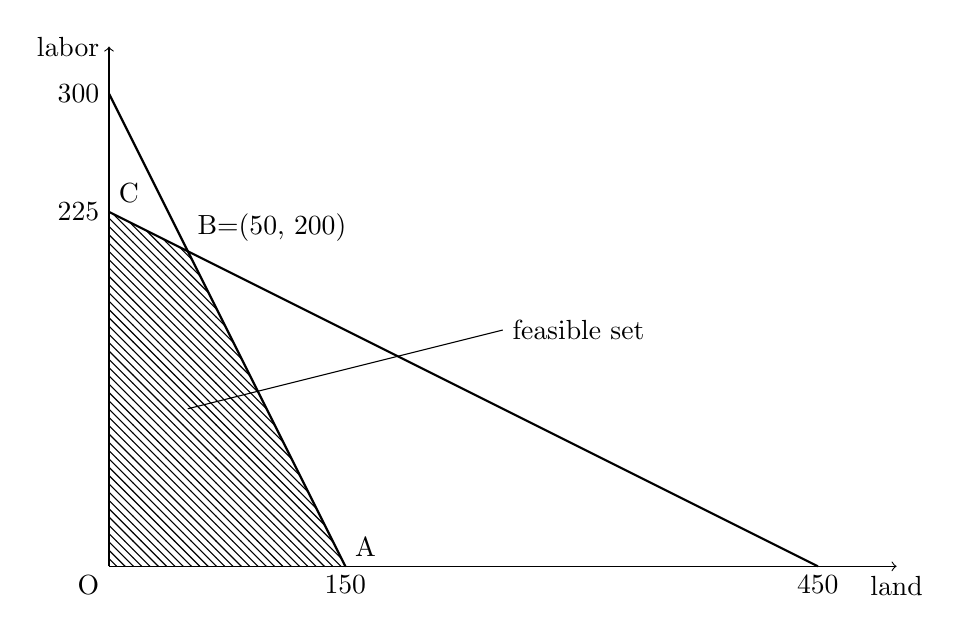
\begin{tikzpicture}[scale=0.02]
    % 绘制坐标轴
    \draw[->] (0,0) -- (500,0) node[below] {land};
    \draw[->] (0,0) -- (0,330) node[left] {labor};
    \draw[black] (0,0) node[below left] {O};


    \draw[thick,black] (0,225) -- (450,0) ;  % 全部用于生产牛肉
    \draw[thick,black] (0,300) -- (150,0) ;  % 全部用于生产小麦

\filldraw [black] (150,0) circle (1pt) node[below] {150} node[above right] {A};
\filldraw [black] (450,0) circle (1pt) node[below] {450};
\filldraw [black] (0,225) circle (1pt) node[left] {225} node[above right] {C};
\filldraw [black] (0,300) circle (1pt) node[left] {300};
\filldraw [black] (50,200) circle (1pt) node[above right] {B=(50, 200)};

    \coordinate (O) at (0,0);
    \coordinate (A) at (150,0);
    \coordinate (B) at (50,200);
    \coordinate (C) at (0,225);
    
    % 使用shade命令填充四边形,创建阴影效果
    %\fill[color=gray!50] (O) -- (A) -- (B) -- (C) -- cycle;
    \fill[pattern = north west lines] (O) -- (A) -- (B) -- (C) -- cycle;
    
\draw[black] (50,100) -- (250,150) node[right] {feasible set};

\end{tikzpicture}
\caption{Production and unemployment} %最终文档中希望显示的图片标题
\label{Fig3.1} %用于文内引用的标签
\end{figure}

Along AB, (\ref{equa3.14}) holds as an equation, while along BC, (\ref{equa3.15}) does. Only at B do both hold as equations. Everywhere else, there is unemployment
of factor or the other.

You might be tempted to assume that is will be optimum to have full employment, and achieve production at B with $x=50$ and $y=200$. However, that is not necessarily so.

Suppose the society has an objective or social welfare function defined over the quantities of the two goods of the simple form we have used before:
\begin{equation} \label{equa3.16}
W(x,y ) = \alpha \ln x + \beta \ln y
\end{equation}
where $\alpha$ and $\beta$ are given positive constants, and $(\alpha + \beta)=1$.

We know from the intuition developed in the previous example that not-negativity constraints on $x$ and $y$ are not going to be binding. So let us leave them out from the start. Write the Lagrange multiplier for the constraint (\ref{equa3.14}) as $\lambda$ and that for (\ref{equa3.15}) as $\mu$. Form the Lagrangian
\begin{equation*}
L(x,y,\lambda, \mu) = \alpha \ln x + \beta \ln y + \lambda [300-2x-y] + \mu[450-x-2y]
\end{equation*}
The first-order conditions are
\begin{equation} \label{equa3.17}
\alpha /x -2 \lambda - \mu =0
\end{equation}
\begin{equation} \label{equa3.18}
\beta /y - \lambda - 2\mu =0
\end{equation}
and
\begin{equation} \label{equa3.19}
300 -2x - y \geq 0, \quad \lambda \geq 0, \quad \mbox{with complementary slackness}
\end{equation}
\begin{equation} \label{equa3.20}
450 -x - 2y \geq 0, \quad \mu \geq 0, \quad \mbox{with complementary slackness}
\end{equation}

Between (\ref{equa3.19}) and (\ref{equa3.20}) we have four possible patterns of equations and inequalities. We should suspect that it is not going to be sensible to keep \textit{both} factors less than fully employed, that is, to have $\lambda=0$ and $\mu=0$. Let us check this out: using $\lambda=0=\mu$ in (\ref{equa3.17}) and (\ref{equa3.18}) would give $\alpha=0=\beta$, and that is not so. Therefore this case is ruled out, and we are left with three.

First consider the case, $\lambda=0$ and $\mu >0$, which I shall label Case (i). Here (\ref{equa3.17}) gives $x=\alpha /\mu$ and (\ref{equa3.18}) gives $y=\beta/ (2\mu)$. Since $\mu >0$, (\ref{equa3.20}) then becomes
\begin{equation*}
450 = x+ 2y = (\alpha + \beta)/\mu, \quad \mbox{or} \quad \mu = 1/450
\end{equation*}
Then $x=450 \alpha$ and $y=225 \beta$.

It remains to check out if the feasibility condition in (\ref{equa3.19}) is true. We need
\begin{equation*}
300 \geq 2x+y=900\alpha + 225\beta = 900-675\beta, \quad \mbox{or} \quad \beta \geq 8/9
\end{equation*}

The other cases can be checked out in the same way, and I shall merely state the results:

If $\lambda>0$ and $\mu=0$ (Case (ii)), we get $x=150\alpha$, $y=300\beta$. The case is internally consistent if $\beta \leq 2/3$.

If $\lambda>0$ and $\mu>0$ (Case (iii)), we get the full employment point $x=50$ and $y=200$. This case is internally consistent if $2/3 < \beta < 8/9$.

The solution gives several useful insights. Once again, the range of parameters splits nicely into exhaustive and mutually exclusive regions, in each of which just one of the cases yields a candidate for optimality. For low values of $\beta$, the solution lies along the line AB. Then there is a middle range where the solution stays at the point B. Finally, for high values of $\beta$ the solution lies along the line BC.

The social indifference curves for the objective function (\ref{equa3.16}) are like hyperbolas. The higher is the weight $\beta$ attached to $y$ (relative to the weight of $x$), the more willing is society to sacrifice $x$ for $y$, that is, the flatter are the hyperbolas. Therefore for low $\beta$ we get a tangency of a social welfare contour and the production possibility set along the segment AB, for medium values we have a corner solution at B, and for high values a tangency along BC.

Next note that at any point along AB (except B), it is optimal to keep some land unemployed. To see why, note that the goods have fixed coefficients of input requirements, and wheat requires relatively more labor. If we wish to use the unemployed land, we must do so by producing less wheat and more beef. To try it the other way round would increase the labor requirement, but labor is already fully employed. But this is a situation with a relatively low $\beta$; beef is not highly valued relative to wheat, and the required sacrifice of wheat is not worth while.

If enough substitution in production were possible, then the difficulty would not arise and both factors could be fully employed. The unemployment in this setting is a consequence of the rigid technology, not of any effective demand failures or coordination failures.

Finally, look again at the complementary slackness conditions (\ref{equa3.19}) and (\ref{equa3.20}). If one factor is not fully employed at the optimum, then the Lagrange multiplier for its constraint is zero. In Chapter 1, the multiplier on the consumer's budget constraint was the marginal utility of money. In the same way, each multiplier in this problem gives the effect on social welfare of having another marginal unit of that factor. Then complementary slackness becomes economically quite intuitive: if it is optimal not to employ the available amount fully, then an increment must be worthless. In the next chapter I shall develop this idea in more detail.

\section*{Exercises}

\subsubsection*{\textit{Exercise 3.1: Rationing}}

Suppose a consumer has the utility function
\begin{equation} \label{equa3.21}
U(x_1, x_2, x_3) = \alpha_1 \ln (x_1) + \alpha_2 \ln (x_2) +\alpha_3 \ln (x_3)
\end{equation}
where the $\alpha_j$ are positive constants summing to one. The budget constraint is
\begin{equation*}
p_1 x_1 + p_2 x_2 + p_3 x_3 \leq I
\end{equation*}
In addition, the consumer faces a rationing constraint: he is not allowed to buy more than $k$ units of good 1.

Solve the optimization problem. Under what condition on the various parameters is the rationing constraint binding?

Show that when the rationing constraint binds, the income that the consumer would have liked to spend on good 1 but cannot do so is now split between goods 2 and 3 in the proportions $\alpha2 : \alpha_3$. Would you expect rationing of bread purchases to affect demands for butter and rice in this way? What is the property of the utility function (\ref{equa3.21}) that produces the result, and how would you expect the bread-butter-rice case to differ?

\subsubsection*{\textit{Exercise 3.2: Distribution Between Envious Consumers}}

There is a fixed total $Y$ of goods at the disposal of society. There are two consumers who envy each other. If consumer 1 gets $Y_1$ and consumer 2 gets $Y_2$, their utilities are
\begin{equation*}
U_1 = Y_1 - k Y_2^2,  \quad   U_2 = Y_2 -k Y_1^2
\end{equation*}
where $k$ is a positive constant. The allocation must satisfy $Y_1 + Y_2 \leq Y$, and maximize $U_1 + U_2$.

Show that if $Y > 1/k$, the resource constraint will be slack at the optimum. Interpret the result.

\subsubsection*{\textit{Exercise 3.3: Investment Allocation}}

A capital sum $C$ is available for allocation among $n$ investment projects. If the non-negative amount $x_j$ is allocated to project $j$ for $j=1,2,\dots,n$, the expected return from this portfolio of projects is
\begin{equation*}
\sum_{j=1}^n [ \alpha_j x_j - \dfrac{1}{2} \beta_j x_j^2 ]
\end{equation*}
The allocation is to be chosen to maximize this.

Find the first-order necessary conditions from the Kuhn-Tucker Theorem. Define
\begin{equation*}
 H= \sum_{j=1}^n (\alpha_j/ \beta_j), \quad K=\sum_{j=1}^n (1/\beta_j)
\end{equation*}
Show that

(i) If $C>H$, then a part of the total sum available is left unused.

(ii) If $\alpha_j > (H-C)/K$ for all $j$, then every project will receive some funding.

(iii) If any project receives zero funding, then it must have a lower $\alpha$ than any project that gets some funding.



\chapter{Shadow Prices}

\section*{Comparative Statics}

Lagrange's methods, and its extensions and generalizations in Chapter 3, all introduce an undetermined multiplier for each constraint. The values of these multipliers are found as a part of the solution. The heuristic discussion of the consumer choice problem in Chapter 1 offered an economic interpretation for its Lagrange multiplier: it was the marginal utility of income. In Chapter 2 and 3 I hinted that a similar interpretation holds much more generally for constrained optimization problem. That is the focus of this chapter.

A constrained optimization problem has several parameters as data. In the maximization of $F(x)$ subject to $G(x)=c$, the parameter $c$ is an obvious example. There are also other parameters that appear in the definitions of the functions $F$ and $G$, for example the weight $\alpha$, $\beta$ and the prices, in the examples and exercises of Chapter 2. Economists often need to know how the solution to the problem will change if these parameters take different values. In consumer theory, we discuss the income and substitution effects of price changes by comparing the optimum choices for different budget lines. In the theory of a firm's production and supply, its marginal cost is the difference between the costs of producing two different levels of output when the firm chooses the least-cost imput mix for each output level. The general method of comparing solutions for various parameter changes is called \textit{comparative statics}, and the importance of Lagrange multipliers lies in the fact that they provide the answer to a very important comparative static question.

\section*{Equality Constraints}

Let us begin in the simple setting of Chapter 2, with two choice variables $(x_1, x_2)$, an objective function $F(x)$, and one equality constraint $G(x)=c$. Let $\bar{x}$ denote the optimum choice, and $v=F(\bar{x})$ the highest attainable value. Now suppose $c$ increases by an infinitesimal amount $dc$. Let $\bar{x}+ d\bar{x}$ be the new optimum choice, and $v+dv$ the new optimum value.

Note a slight difference between the usage here and that of Chapter 2. There the aim was to test $\bar{x}$ for optimality, and we did this by considering \textit{arbitrary} deviations $dx$ from it. This led us to the first-order necessary conditions that held at the optimum $x$. Now the increment $d\bar{x}$ is not arbitrary; it is the \textit{optimum} small change in the choice, arising in response to a small change in the parameters.

For these small changes, we can use the first-order Taylor approximations to the changes in the values of $F$ and $G$. We have
\begin{equation*}
\begin{array}{rl}
dv = & F(\bar{x} + d\bar{x} ) - F(\bar{x}) \\
   = & F_1(\bar{x}) d\bar{x}_1 + F_2(\bar{x}) d\bar{x}_2 \\
   = & \lambda [ G_1(\bar{x}) d\bar{x}_1 + G_2(\bar{x}) d\bar{x}_2 ] \\
   = & \lambda [ G(\bar{x} + d\bar{x} ) - G(\bar{x}) ] \\
   = & \lambda [(c+dc)-c] = \lambda dc
\end{array}
\end{equation*}
In the derivation, the second and the fourth lines are the Taylor approximations, the third line uses the first-order condition (\ref{equa2.6}), and the fifth line uses the constraint (\ref{equa2.1}). The result can now be written
\begin{equation} \label{equa4.1}
dv / dc = \lambda
\end{equation}

Thus the multiplier is the rate of change of the maximum attainable value of the objective function with respect to a change in the parameter on the right-hand side of the constraint. Now we can see the marginal utility of income in Chapter 1 as a special case of this more general result.

The case of several choice variables and many equation Constraints is no harder. In vector-matrix notation, the argument is in fact identical. Look at the first section of Chapter 3. Let the right-hand side of the vector constraint change by $dc$, and write $d\bar{x}$ for the resulting change in the optimum vector $\bar{x}$. Then
\begin{equation*}
\begin{array}{rl}
dv = & F(\bar{x} + d\bar{x} ) - F(\bar{x}) = F_x(\bar{x}) d\bar{x}  \\
   = & \lambda G_x(\bar{x}) d\bar{x} = \lambda [ G(\bar{x} + d\bar{x} ) - G(\bar{x}) ] = \lambda dc
\end{array}
\end{equation*}
Pause a moment to check the sizes of the various vectors and matrices being multiplied. For example, in the first expression of the second line, $\lambda$ is an $m$-dimensional row vector, $G_x(\bar{x})$ is an $m \times n$ matrix, and $d\bar{x}$ is an $n$-dimensional column vector. The final result is the product of the row vector $\lambda$ and the column vector $dc$ of equal dimensions $m$; therefore it is a scalar. In fact it is the inner product of the two vectors:
\begin{equation*}
 \lambda dc = \sum_i \lambda_i dc_i
\end{equation*}

The result is important enough to be stated separately for reference:

\textit{Interpretation of Lagrange Multipliers:} If $v$ is the maximum of $F(x)$ subject to a vector of Constraints $G(x)=c$, and $\lambda$ is the row vector of multipliers for the constraints, then change $dv$ that results from an infinitesimal change $dc$ is given by
\begin{equation} \label{equa4.2}
dv = \lambda dc
\end{equation}

It should be stressed that (\ref{equa4.2}) gives only the first-order or linear approximation to the change in $v$ if the change in $c$ is more than infinitesimal. For such changes, we can carry the Taylor expansion to higher orders and find a closer approximation. This will be done, although for a different purpose, in Chapter 8.

\section*{Shadow Prices}

To illustrate and explain (\ref{equa4.2}), consider a planned economy for which a production plan $\bar{x}$ is to be chosen to maximize a social welfare function $F(x)$. The vector of the plan's resource requirement is $G(x)$, and the vector of the available amounts of these resources is $c$. Suppose the problem has been solved, and the vector of the Lagrange multipliers $\lambda$ is known. Now suppose some power outside the economy puts a small additional amount $dc_1$ of the first resource (say labor) at its disposal. The optimization problem can be solved afresh with the new labor constraint to determine the new pattern of production. But we know the resultant increase in social welfare without having to do this calculation: it is simply $\lambda_1 dc_1$. We can then say that the multiplier $\lambda_1$ is the marginal product of labor in this economy, measured in units of its social welfare. This is clearly a vital piece of economic information, and that is why Lagrange's method and his multipliers are so important in economics.

If there is only one scarce input, then a paraphrase of the argument of Chapter 1 yields another very instructive way of looking at this result. Suppose we use the additional labor input to raise the quantity of a particular good, say good $j$, leaving the outputs of all the other goods unchanged. Since we are assuming full employment of labor in both situations, the increase $d\bar{x}_j$ in the output of the chosen good must satisfy
\begin{equation*}
G_j^1(\bar{x}) d\bar{x}_j = dc_1, \quad \mbox{or} \quad d\bar{x}_j = dc_1 / G_j^1(\bar{x})
\end{equation*}
The resultant increases in social welfare is
\begin{equation*}
F_j(\bar{x}) d\bar{x}_j =  [F_j(\bar{x})/ G_j^1(\bar{x})]  dc_1
\end{equation*}
The condition of optimality (\ref{equa2.5}) says that the ratio in the square brackets should be the same for all $j$. Therefore the effect of the marginal increase in labor supply on social welfare is independent of how the extra labor is used. That is why we can speak unambiguously of the marginal product of labor.

Now suppose the additional labor can only be used at some cost. The maximum the economy is willing to pay in terms of its own social welfare units is clearly $\lambda_1$ per marginal unit of $c_1$. Any smaller payment leaves it with a positive net benefit from using the extra labor; for any larger payment the cost exceeds the benefit. In this natural sense, the Lagrange multiplier is the \textit{demand price}  the planner places on labor services. A price expressed in units of social welfare may seem strange, but a minor modification brings it into familiar light. Consider some other resource, say land, and number it 2. Now suppose the economy is offered the services of an extra $dc_1$ of labor, but asked to give in return the services of $dc_2$ of land. The net gain in social welfare from this transaction is $(\lambda_1 dc_1 - \lambda_2 dc_2)$. Therefore the most land the planner is willing to give up is $(\lambda_1/ \lambda_2 )dc_1$. Then it is equally natural to call the ratio $\lambda_1/ \lambda_2$ the demand price of a unit of labor measured in units of land. You know from microeconomic theory that \textit{relative} prices rather than \textit{absolute} ones govern market exchange; similarly the relative magnitudes of the Lagrange multipliers for different resources govern the planner's willingness to exchange one resource for another.

If a neighboring economy has a different trade-off between the two resources on account of differences in their relative availability or technology, then there is a possibility of mutually advantageous trade in factor services between the two. (Even if factor services cannot be traded, exchange of goods made using these factors can secure some or even all of the mutual gain, but details of that would take us too far into the theory of international trade.)

Of course, the internal organization of the economy need have nothing to do with prices, and the Lagrange multiplier for the labor constraint need not equal the wage that is actually paid for each man-hour. Labor may simply be directed to various tasks in a command economy. (There are serious conceptual and practical problems in so doing, as most Soviet-style economics have now realized, but that again is another story.) But the plan implicitly places values on the resources, and the planner's understanding of the economy and of its possible bottlenecks will be improved by paying attention to the multipliers that relect these values.

Now consider an economy that does allocate resources using markets. In equilibrium, the prices are such that the demands and supplies chosen by individuals solving their own constrained maximization problems are equal in the aggregate. Now suppose an economist sets out to evaluate the performance of the economy using some given criterion. To get a comparison standard, he will solve the planning problem of maximizing this criterion function subject to constraints arising from the economy's resource availability, technology, and information transmission. The solution will include a vector of Lagrange multipliers for the resource constraints.

You may think there is little reason why the market should replicate this planned allocation, and equally little reason why the Lagrange multipliers should have anything to do with the market prices. But there are important cases where the optimum can be replicated in the market, and the Lagrange multipliers are proportional to the market prices of the resources: the relative prices equal the corresponding ratios of multipliers. In such cases the economist is tempted to say that the economy is guided by an `invisible hand' to his planned optimum. Such a case is worked out in detail in Example 4.1. If rests on many special assumptions whose validity is often doubtful, and most of modern economic theory is concerned with questions of what happens when those assumptions are not met. But the case has great importance as the point of departure for all such analysis, and as a practical matter many people believe in the optimality of the market mechanism. Therefore it deserves careful study.

To evoke the connection with prices, and yet maintain a conceptual distinction from market prices, Lagrange multipliers are often called \textit{shadow prices}.

\section*{Inequality Constraints}

An economic question now arises. We expect prices to be non-negative, but so far we have seen no reason why the shadow prices (Lagrange multipliers) should be non-negative. In the planning application used in the above exposition, the multipliers measured the increase in social welfare resulting from increased availability of scarce resources. Having more of a resource leaves all previous production opportunities available and adds some new ones. This should allow the planner to achieve at least as high a level of social welfare, and in most instances a higher level. In the same way, in the general problem of constrained optimization, a relaxation of the constraint should be a desirable thing. Can the mathematics confirm this intuition?

One difficulty is that in the general formulation of the problem with equality constraints, an increase in the right-hand side of a constraint equation need not mean a relaxation of the constraint. Trivially, we could have written the constraint $G^i(x)=c_i$ as $-G^i(x)=-c_i$, and an increase in the right-hand side of the new form would be a decrease in the quantity $c_i$ of resource $i$. Also, not all of the constraints need be ones of resource availability. For example, we might want to maximize the amount of investment while ensuring a minimum acceptable provision of some consumer goods. Now an increase in this stipulated minimum tightens the economic constraint, so a smaller amount of investment can be squeezed out and the multiplier is negative. Here the multiplier is like the slope of a transformation function (consumption into investment). We should expect such a curve to be downward-sloping, and should interpret \textit{minus} the slope as the shadow price.

These examples show that if we want non-negative shadow prices, we must be careful to write the constraints in such a way that an increase in the right-hand side does relax the restrictions on the choice.

There is another, more important, consideration. There may be cases in which the marginal value of a resource turns negative beyond a point. For example, too many workers may simply interfere with one another's effort. In such a case, a further increase in the quantity of the resource will mean a lower maximum value of the objective function and a negative multiplier. But in such a situation, it would be better not to use the resource in such excessive amounts even if it is available. Exercise 3.2 considered a situation where it was optimal to throw away some quantity of a good in the face of overwhelming envy effects. Mathematically, the equality constraint forces use of the entire amount available. If the constraint were an Inequality, $G^i(x) \leq c_i$, then we would have the freedom to leave resources idle when this serves the goals of optimization.

In practice there may be some costs of leaving resources idle. Unemployment of labor might be thought to be socially undesirable, and some capital, especially brains, can rust when unused. In such situations we should include these costs in the objective function. Provided this has been done, there is no economic reason to deny ourselves the freedom of leaving some part of the resource endowment unused if this leads to a better outcome.

This discussion has an exact parallel in market prices, too. If some `goods' are actually `bads', we expect them to have negative prices. More generally, it is the assumption of \textit{free disposal} that ensures non-negative prices.

The Kuhn-Tucker Theorem stated in Chapter 3 gives the first-order necessary conditions for maximization subject to Inequality constraints. It immediately confirms this intuition. The condition (\ref{equa3.10}) says that the vector of the Lagrange multipliers is non-negative. It yields a further result of considerable importance. The vector inequality $\lambda \geq 0$ shows complementary slackness with $L_\lambda \geq 0$, which is just another way of writing $G(x) \leq c$. For every $i$, at least one of the pair
\begin{equation*}
G^i(x) \leq c_i, \quad \lambda_i \geq 0
\end{equation*}
holds as an equation. If resource $i$ is not fully used, then its shadow price is zero; a resource with a positive shadow price must be fully used.

This supports and completes the interpretation of shadow prices as the marginal value products of the resources. If part of some resource is already idle, then any increment in it will also be left idle. The maximum value of the objective function will not change, and the shadow price will be zero. On the other hand, a positive shadow price means that a marginal increment in resource availability can be put to good use. Then none of the amount originally available can have been left idle in the original plan. You should return to the account of technological unemployment in Example 3.2 and examine the results there in this light.

There is just one tricky point to be taken care of. Suppose $c_i$ is much that resource $i$ is just on the point of becoming superfluous at the margin. This amount is fully used, but any increment will be left unused. Complementary slackness does not tell us whether the multiplier will be positive or zero at this point. In fact the answer is specific to each problem, and depends on whether the slope of the maximum value $v$ shown as a function of $c_i$ drops smoothly or suddenly to zero at the borderline point.

\begin{figure}[!htp]  % 常见htbp  here top bottom p表示浮动  !表示忽略“美学”标准
 \centering
 \subfloat[ ] %第一张子图
 {
   \begin{minipage}{0.5\linewidth}
\centering
        \begin{tikzpicture}[scale=2]
    % 绘制坐标轴
    \draw[->] (0,0) -- (2.5,0) node[below] {$c_i$};
    \draw[->] (0,0) -- (0,2.5) node[left] {$v$};
    \draw[black] (0,0) node[below left] {O};

    \draw[domain=0.2:1,smooth,variable=\x] plot ({\x},{( 4 * \x -2 * \x * \x)}) ;
    \draw[] (1,2) -- (2,2) ; 
        \end{tikzpicture}
   \end{minipage} }
 \subfloat[ ] %第二张子图
   {
   \begin{minipage}{0.5\linewidth}
\centering
       \begin{tikzpicture}[scale=2]
    % 绘制坐标轴
    \draw[->] (0,0) -- (2.5,0) node[below] {$c_i$};
    \draw[->] (0,0) -- (0,2.5) node[left] {$v$};
    \draw[black] (0,0) node[below left] {O};

    \draw[domain=0.4:1,smooth,variable=\x] plot ({\x},{( 2.5 * \x -0.5)}) ;
    \draw[] (1,2) -- (2,2) ; 

\filldraw [black] (1,2) circle (1pt)   ;
      \end{tikzpicture}
   \end{minipage} }
 \caption{Resource quantities and shadow prices} \label{Fig4.1} 
\end{figure}


Figure \ref{Fig4.1} shows both possibilities. In (a) the drop is smooth, and the multiplier at the point in question is zero. In (b) the drop is sudden, and any value of $\lambda_i$ between the slope of the curve to the left and its slope to the right (zero) will serve at athe point of transition. This happens in the context of linear programming (Example 7.1).

\section*{Examples}

\subsubsection*{\textit{Example 4.1: The Invisible Hand - Distribution}}

Consider the stage of planning where the production of the various goods is already known, and the only remaining question is that of distributing them among the consumers. There are $C$ consumers, labeled $c=1,2,\dots, C$, and $G$ goods, labeled $g=1,2,\dots,G$. Let $X_g$ be the fixed total amount of good $g$, and $x_{cg}$ the amount allocated to consumer $c$. Each consumer's utility is a function only of his own allocation,
\begin{equation} \label{equa4.3}
u_c = U^c(x_{c1}, x_{c2}, \dots, x_{cG}    )
\end{equation}
Social welfare is a function of these utility levels
\begin{equation*}
w = W(u_{1}, u_{2}, \dots, u_{C}    )
\end{equation*}
The constraints are that for each good, its allocation to the individuals should add up to no more than the total amount available. When the utilities and social welfare are increasing functions, it is clear that no goods are going to be wasted, so we can express the constraints as equations
\begin{equation} \label{equa4.4}
 x_{1g} + x_{2g} + \dots + x_{Cg} = X_g, \quad \mbox{for} \quad g=1,2,\dots,G
\end{equation}
and use Lagrange's Theorem. Let $\pi_g$ be the multiplier for the constraint on good $g$, and form the Lagrangian
\begin{equation*}
L = W[ U^1(x_{11}, \dots, x_{1G}  ), \dots, U^C(  x_{C1}, \dots, x_{CG}  ) ] + \sum_g \pi_g [X_g - \sum_c x_{cg} ]
\end{equation*}
where the arguments of $L$ and the ranges of summation are omitted for brevity.

When deriving the first-order conditions, we must differentiate $L$ with respect to every $x_{cg}$ using the chain rule. This gives
\begin{equation} \label{equa4.5}
 (\partial W / \partial u_c)  (\partial U^c / \partial x_{cg}) - \pi_g =0
\end{equation}

All the partial derivatives are to be evaluated at the optimum as usual; I omit them for case of notation. The multipliers $\pi_g$ are also obtained as a part of the solution.

Now suppose the $\pi_g$ are made the prices of the goods. Every consumer $c$ is given a money income $I_c$, and allowed to choose his consumption vector to maximize his utility \ref{equa4.3} subject to the budget constraint
\begin{equation} \label{equa4.6}
  \pi_1 x_{c1} + \pi_2 x_{c2} + \dots + \pi_G x_{cG} = I_c
\end{equation}
This optimization will be characterized by the conditions
\begin{equation} \label{equa4.7}
   \partial U^c / \partial x_{cg} = \lambda_c \pi_g
\end{equation}
for all $g$ and $c$. As usual, $\lambda_c$ is the marginal utility of income for consume $c$.

If we compare \ref{equa4.5} and \ref{equa4.7}, we see that they coincide provided we set
\begin{equation} \label{equa4.8}
 \partial W/ \partial u_c = 1/\lambda_c, \quad \mbox{or} \quad (\partial W/ \partial u_c ) \lambda_c =1
\end{equation}
for all $c$. This can be done by adjusting the money incomes $I_c$. The left hand side of the second equation in (\ref{equa4.8}) is simply the marginal effect on social welfare of giving a unit of income to consumer $c$; it is the marginal effect on $c$'s own utility \textit{times} the effect of a unit of his utility on social welfare.

In other words, the distribution of income should be arranged so that at the margin the social value of every consumer's income is the same. Once this is done, they can be left free to choose their actual consumption bundles. This is the `invisible hand' result for the distribution problem.

The argument comparing first-order conditions is not fully rigorous, but better proofs exist. The important thing is to recognize the crucial assumptions that lead to the result. Here the most important is the dependence of every consumer's utility only on his own consumption quantities. If one consumer's utility depends on another's consumption, this is called an `external effect' or `externality'. Such effects can interfere with the simple decentralization of consumption through prices. In essence, we must charge each consumer not just for the scarcity value of his consumption, but also for the harm his consumption causes to the utility of others (or pay him for the benefit he confers on others). Such prices can be person-specific, and the market implementation becomes much more complicated.

\subsubsection*{\textit{Example 4.2: Duty-Free Purchases}}

Let us turn from the dreary image that central planning and income distribution always invoke, to the consumption decision of a jet-setter. He can buy various brands of liquor at his hometown store, or at the duty-free stores of the various airports he travels through. The duty-free stores have cheaper prices, but the total quantity he can buy there is restricted by his home country's customs regulations.

There are $n$ brands. Let $p$ be the row vector of hometown prices and $q$ that of duty-free prices. The duty-free prices are uniformly lower: $ q \ll p$. Let $x$ be the column vector of his hometown purchases and $y$ that of the duty-free. Suppose he travels and entertains enough in a year that we can regard the quantities as continuous variables, not restricted to integer numbers of bottles. The integer problem gives similar results, but needs different techniques.

Let us simplify the problem by leaving aside the problem of choice between liquor as a whole and all other goods. Thus we take the income he has decided to spend on liquor during the year as fixed, say $I$. The budget constraint then becomes
\begin{equation} \label{equa4.9}
  px + qy \leq I
\end{equation}

Suppose during the year our jet-setter is allowed to import $K$ bottles of liquor duty-free. This constraint is
\begin{equation*}
 y_1 + y_2 + \dots + y_n \leq K
\end{equation*}
To simplify the notation, let $e$ be the row vector with every component equal to one. Then the left-hand side is just the product $ey$, and the constraint can be written
\begin{equation} \label{equa4.10}
 e y \leq K
\end{equation}

Unless the consumer is satiated within his duty-free allowance (an unlikely story), both constraints are going to hold as equations. But we should expect that it will be optimal to buy some brands only at duty-free stores and others only at hometown stores. Therefore we must remember that $x$ and $y$ are restricted to be non-negative.

Utility depends only on the total consumption $c=x+y$. Therefore the Lagrangian is
\begin{equation*}
  L = U(c )+ \lambda[I- px-qy] + \mu [K-ey]
\end{equation*}
The first-order conditions are given by Lagrange's Theorem for non-negative variables in Chapter 3. For each $j$, we have
\begin{equation} \label{equa4.11}
 \partial L / \partial x_j  \equiv   \partial U / \partial c_j - \lambda p_j \leq 0, \quad x_j \geq 0
\end{equation}
with complementary slackness, and
\begin{equation} \label{equa4.12}
 \partial L / \partial y_j  \equiv   \partial U / \partial c_j - \lambda q_j -\mu \leq 0, \quad y_j \geq 0
\end{equation}
also with complementary slackness.

These inequality pairs permit $2^{2n}$ patterns of equations and zeros, and sorting them out systematically would be hopeless. But a search assisted by economic intuition quickly reveals the solution.

Can some brand $j$ be bought in positive amounts at both kinds of stores? If so, the equations that emerge from (\ref{equa4.11}) and (\ref{equa4.12}) are
\begin{equation*}
 \partial U / \partial c_j - \lambda p_j = 0 = \partial U / \partial c_j  -\lambda q_j - \mu
\end{equation*}
or
\begin{equation} \label{equa4.13}
\lambda p_j = \partial U /\partial c_j = \lambda q_j + \mu
\end{equation}

Save by coincidence, this can hold for at most one $j$. If it were true for $j=1$ and 2, say, we would have
\begin{equation*}
 \lambda(p_1 - q_1) = \mu = \lambda (p_2 - q_2)
\end{equation*}
Since we are supposing the consumer is not satiated, $\lambda$ is positive and
\begin{equation*}
   p_1 - q_1 = p_2 - q_2
\end{equation*}
With given prices, this can occur only by chance. This argument not only narrows down our search, but also tells us that the \textit{absolute} price differences between the two sets of prices will have a lot to do with the optimal purchases decision.

Now suppose brand $j$ is bought only in the hometown store. With $x_j >0$ and $y_j=0$, we have
\begin{equation} \label{equa4.14}
 \partial U / \partial c_j  = \lambda p_j
\end{equation}
and
\begin{equation} \label{equa4.15}
 \partial U / \partial c_j \leq  \lambda q_j + \mu
\end{equation}

Of these, (\ref{equa4.14}) is familiar, but even it benefits from a reinterpretation. The left-hand side is just the marginal utility of brand $j$. The right-hand side is the marginal opportunity cost of buying it at the hometown store: to do so takes $p_j$ of income which cannot then be used for other purchases, and the utility value of this much income is $\lambda p_j$.

This in turn casts light on (\ref{equa4.15}). Its right-hand side is the marginal opportunity cost of buying a unit of brand $j$ at a duty-free store. This requires $q_j$ of income having utility value $\lambda q_j$. But is also uses up a unit of the duty-free allowance, which has the shadow price $\mu$. The total opportunity cost of the purchases is the sum of these two components. If the brand is not bought at the duty-free store, it must be because the opportunity cost of so doing exceeds the marginal utility from its consumption.

Now the principle is clear: buy each brand at the outlet with the lower opportunity cost. Note that
\begin{equation*}
  \lambda q_i +\mu < \lambda p_i   \quad \mbox{if and only if} \quad p_i -q_i > \mu / \lambda
\end{equation*}
Therefore our jet-setter should rank the brands by their absolute price differences in the two kinds of stores. The brands with the largest price differences are bought at the duty-free stores, and those with the smallest price differences, at the hometown store. The meeting-point of the two is chosen so as to use up the duty-free allowance. There may be at most one brand that is bought at both kinds of stores.

Incidentally, if the duty-free allowance restricts the total value $qy$ of purchases instead of the quantity $cy$, then the solution will be similar, but the brands will be ranked by their \textit{relative} price differences instead of the \textit{absolute} ones. I shall leave this case for the readers to work out as an exercise.

\section*{Exercises}

\subsubsection*{\textit{Exercise 4.1: The Invisible Hand - Production}}

Continue with the notation of Example 4.1, but now allow production of the goods. Let there be $F$ factor inputs, available in fixed quantities $Z_f$ for $ f = 1,2,\dots, F$. If $z_{fg}$ of factor $f$ is used in the production of good $g$, the output $X_g$ is given by the production function
\begin{equation} \label{equa4.16}
  X_g = \Phi^g (z_{1g}, z_{2g}, \dots, z_{Fg})
\end{equation}

Add these constraints to the earlier problem. Verify that the first-order conditions of optimum distribution are the same as before, but new conditions for optimum factor allocation are added. Interpret the Lagrange multiplier. Can production be decentralized, with one firm producing each good? Show that the sum of the incomes $I_c$ handed out to the consumers equals the value of aggregate output.

\subsubsection*{\textit{Exercise 4.2: The Invisible Hand - Factor Supplies}}

Now let even the factor supplies $Z_f$ be a part of the optimization. Suppose each consumer $c$ supplies $z_{cf}$ of factor $f$. These amounts affect his utility adversely; there is disutility from supplying factors.

Find the first-order conditions. Interpret the Lagrange multipliers and discuss the implementation of the optimum in a market framework.

Now you must distinguish two source of income for the consumers: their earnings from the factor services they supply, and the lump sums $I_c$ they get from the government. These lump sums must now be varied (in a person-specific way) to attain the condition (\ref{equa4.8}). Show that the total of the lump sums handed out to the consumers equals the total profit in production, that is, the value of output minus the payments to the factors.

\subsubsection*{\textit{Exercise 4.3: Borrowing and Lending}}

Consider a consumer planning his consumption over two years. He will have income $I_1$ during the first year and $I_2$ during the second. In each year there are two goods to consume. In year 1, the prices are $p_1$ and $q_1$, and the corresponding quantities $x_1$ and $y_1$. In year 2, we similarly have $p_2$ , $q_2$ and $x_2$ , $y_2$. The utility function is
\begin{equation*}
 u_1 = \alpha_1 \ln (x_1) + \beta_1 \ln (y_1) + \alpha_2 \ln (x_2) + \beta_2 \ln (y_2)
\end{equation*}
This is to be maximized subject to two budget constraints, one for each year.

Solve this problem, and find the multipliers $\lambda_1$ and $\lambda_2$ for the two constraints. Examine how they depend on money income and other parameters of the problem.

How much more of year-2 income will the consumer require if he is to give up $dI_1$ of year-1 income? In other words, what is the rate of return needed to induce him to save a little? You would expect borrowing and lending institutions arise in an economy populated by such consumers. What governs who will borrow and who will lend?














\chapter{Maximum Value Functions}

The last chapter introduced the concept of comparative static, and used it to interpret the Lagrange multipliers as the rates of change of the maximum attainable value of the objective function with respect to the right-hand sides of the constraint equations. Many other parameters enter the objective function and the constraint functions, and the maximum attainable value of the objective function depends on them all. The method used before can be adapted to understand the nature of this more general dependence. That is the object of this chapter. As there, I shall begin with the case where all constraints are exact equalities, and consider inequality constraints later.

\section*{Parameters in the Objective Function}

Consider first the case where the parameters affect the maximand alone. A common example is a producer who chooses a mix of inputs to minimize the cost of producing a given target output. The prices of the inputs are parameters that affect his objective function. But the constraint, which says that the chosen inputs should yield the desired output, involves only the production function and not the prices. As another example, consider a small country that chooses its production pattern to maximize the national product evaluated at world prices; now these prices are parameters that affect the maximand. More generally, suppose a vector $\theta$ of parameters enters the objective function, so $x$ is chosen to maximize $F(x,\theta)$ subject to the usual vector constraint $G(x)=c$. Lagrange's modification - we now recognize the dependence of $F$ and the Lagrangian on $\theta$. Thus
\begin{equation*}
L(x, \lambda, \theta) = F(x, \theta) + \lambda[c-G(x)]
\end{equation*}
and the optimum $\bar{x}$ satisfies the first-order conditions
\begin{equation*}
L_x(\bar{x}, \lambda, \theta)=0, \quad L_\lambda(\bar{x},\lambda, \theta)=0
\end{equation*}

Write $v$ for the maximum value once again. Suppose $\theta$ changes to $(\theta + d\theta)$. Correspondingly, let the optimum $\bar{x}$ change to $(\bar{x} +d\bar{x} )$, and the maximum value to $(v +dv)$. Using first-order Taylor approximations as in Chapter 4, we can find an expression for $dv$.
\begin{equation} \label{equa5.1}
\begin{array}{rl}
dv & = F(\bar{x} + d\bar{x}, \theta+d\theta) - F(\bar{x}, \theta) \\
   & = F_x(\bar{x}, \theta) d\bar{x} + F_\theta(\bar{x}, \theta) d\theta \\
   & = \lambda G_x(\bar{x}) d\bar{x} + F_\theta(\bar{x}, \theta) d\theta \\
   & = F_\theta(\bar{x}, \theta) d\theta
\end{array}
\end{equation}
In this calculation, the passage from the second to the third line uses Lagrange's first-order condition, and the passage to the last line uses the fact that the value of $G$ stays equal to $c$ in the course of the change in $\theta$.

Once again, for changes in $\theta$ that are large enough to make the first-order approximation invalid, we can carry the series expansion further to find closer approximations to changes in $v$. But the result above has great interest because of its simplicity. It says that to find the first-order change in the maximum value of the objective function in response to changes in parameters that do not affect the constraints, we need not worry about the simultaneous change in the optimum choice $\bar{x}$ itself. All we have to do is to calculate the partial effect of the parameter change, and evaluate the expression at the initial optimum choice.

The cost-minimization problem mentioned above illustrates this well. Suppose $x$ is the vector of inputs, $G$ the production function, and $c$ the required output quantity. Let $\theta$ be the row vector of input prices. Then the producer minimizes $\theta x$, that is,
\begin{equation*}
\mbox{maximizes} F(x,\theta) = -\theta x \quad \mbox{subject to} G(x)=c
\end{equation*}
Write the resulting maximum as $(-v)$. Then (\ref{equa5.1}) gives 
\begin{equation*}
d(-v) =d\theta F_\theta(\bar{x}, \theta) = -d\theta \bar{x}
\end{equation*}
Note that $d\theta$ is a row vector, so we interpret $F_\theta$ as a column vector and write the inner product as shown. The result is 
\begin{equation} \label{equa5.2}
dv = d\theta \bar{x}
\end{equation}

Now $v$ is just the minimum cost of producing output $c$ when input prices are $\theta$. When input prices change, the producer will change his input mix, using less of the inputs that have become relatively more expensive and more of the others. That is, he will substitute along an isoquant of the production function. But the $x$ in (\ref{equa5.2}) is the optimal choice for the original parameter vector $\theta$, not the one for $\theta +d\theta$, or some average. In other words, the first-order change in the cost is just the change in the cost of the original optimum $\bar{x}$, as if fixed coefficients ruled. Another way of looking at this is useful. If we write $v=\theta \bar{x}$ and differentiate, we have
\begin{equation*} 
dv = \theta d\bar{x} + d\theta \bar{x}
\end{equation*}
The first term on the right-hand side is the value of the change in the input mix, using the original prices. But at those prices, the original mix is chosen optimally, therefore the value of any change in it must be zero to the first order. This just leaves the second term, as in (\ref{equa5.2}).

\section*{The Envelope Theorem}

\begin{figure}[!htb] %H为当前位置,!htb为忽略美学标准,htbp为浮动图形
\centering %图片居中
%\includegraphics[width=0.8\textwidth]{./Fig3.1.png} %插入图片,[]中设置图片大小,{}中是图片文件名
\begin{tikzpicture}[scale=0.12]
    % 绘制坐标轴
    \draw[->] (0,0) -- (90,0) node[below] {$\theta$};
    \draw[->] (0,0) -- (0,80) ;
    \draw[black] (0,0) node[below left] {O};

\draw[domain=5:77,smooth,variable=\x,red] plot ({\x},{ 0.01*\x *\x +10}) node[left] {$V(\theta)$};

\draw[domain=7:33,smooth,variable=\x,blue] plot ({\x},{-0.01*\x*\x + 0.8*\x + 2}) node[below] {$F(\bar{x}^1, \theta)$};
\filldraw [black] (20,14) circle (20pt) ;
\draw[dashed,black] (20,14) -- (20,0) node [below] {$\theta_1$} ;

\draw[domain=45:75,smooth,variable=\x,blue] plot ({\x},{-0.01*\x*\x + 2.4*\x - 62}) node[right] {$F(\bar{x}^1, \theta)$};
\filldraw [black] (60,46) circle (20pt) ;
\draw[dashed,black] (60,46) -- (60,0) node [below] {$\theta_2$} ;

\end{tikzpicture}
\caption{The Envelope Theorem} %最终文档中希望显示的图片标题
\label{Fig5.1} %用于文内引用的标签
\end{figure}

The algebra of the previous section is illustrated geometrically in Figure \ref{Fig5.1}. For a particular value of $\theta$, say $\theta_1$, suppose the optimum choice is $\bar{x}^1$. The two curves represent two functions of $\theta$. One is $F(\bar{x}^1, \theta)$, where $x$ is held fixed at $\bar{x}^1$ as $\theta$ varies. The other is the optimum value function linking $v$ and $\theta$, where $x$ is allowed to vary optimally as $\theta$ varies. Formally, this function is defined by
\begin{equation} \label{equa5.3}
V(\theta) = \mathop{\max}_{x} \{  F(x, \theta)| G(x)=c  \}
\end{equation}
which is read as `$V(\theta)$ is the maximum over $x$ of $F(x,\theta)$ subject to $G(x)=c$'. Next write the optimum choice $\bar{x}$ itself as a function $x = X(\theta)$, then we have
\begin{equation*}  
V(\theta) = F(X(\theta), \theta)
\end{equation*}

The two functions $V(\theta)$ and $F(\bar{x}^1, \theta)$ coincide at $\theta_1$, because $x^1$ happens to be the optimal choice there. For other values of $\theta$, unless $\bar{x}^1$ remains the optimal choice, the curve slowing the optimum value function will be higher than that of $F(x^1  ,\theta )$. (In many event, it cannot be lower.) Therefore the two curves should be mutually tangential at $\theta_1$, and that is just what (\ref{equa5.1}) expresses.

Similarly, we could draw the graph of $F(\bar{x}^2, \theta)$, where $\bar{x}^2$ is the optimal choice at $\theta_2$. This would touch the graph of the optimal value function $V(\theta)$ at $\theta_2$. In fact we could draw a whole family of curves of $F(x, \theta)$ for a whole range of fixed values of $x$, each optimal for some $\theta$. No member of this family of curves could ever cross above the graph of $V(\theta)$, and each would be tangential to the optimal value function at that value of $\theta$ where its $x$ happened to be the optimal choice. In other words, the optimal value function is the upper envelope of the family of value functions, in each of which the choice variables are held fixed. That is why the formula (\ref{equa5.1}) is often referred to as the $Envelope Theorem$.

In the cost-minimization application, for example, let a scalar parameter $\theta$ denote the price of just one input. When the vector of input quantities is held fixed, the cost of production is a linear function of $\theta$. The minimized cost as a function of $\theta$ is the lower envelope (no upper, because this is a problem of minimization, not maximization) of all these straight lines, Figure \ref{Fig5.2} shows this.

\begin{figure}[!htb] %H为当前位置,!htb为忽略美学标准,htbp为浮动图形
\centering %图片居中
%\includegraphics[width=0.8\textwidth]{./Fig3.1.png} %插入图片,[]中设置图片大小,{}中是图片文件名
\begin{tikzpicture}[scale=2.5]
    % 绘制坐标轴
    \draw[->] (0,0) -- (4,0) node[below] {$\theta$};
    \draw[->] (0,0) -- (0,4) node[left] {$c$};
    \draw[black] (0,0) node[below left] {O};

\draw[domain=0:3,smooth,variable=\x,red] plot ({\x},{ sqrt{ (6* \x - \x * \x)} }) node[below] {minimum cost};

\draw[domain=0:1.5,smooth,variable=\x, blue] plot ( {\x} , { \x *5 / sqrt(11) + 3 / sqrt(11) } );
\draw[domain=0:2,smooth,variable=\x, blue] plot ( {\x} , { \x *2 / sqrt(5) + 3 / sqrt(5) } ) node[above] {cost line for fixed $x$};
\draw[domain=0:2.8,smooth,variable=\x, blue] plot ( {\x} , { \x * sqrt(2)/4 + 3 / sqrt(2) } );

\filldraw [black] (1/2, {sqrt(11)/2}) circle (1pt) ;
\filldraw [black] (1,{sqrt(5)}) circle (1pt) ;
\filldraw [black] (2,{2*sqrt(2)}) circle (1pt) ;

\end{tikzpicture}
\caption{The minimum cost function} %最终文档中希望显示的图片标题
\label{Fig5.2} %用于文内引用的标签
\end{figure}

The main focus here is on a first=order or tangency property: where the upper envelope meets one member of the family of curves, the two are tangential. In the cost-minimization example, let $x$ denote the quantity of the input whose price $\theta$ is being varied. The slope of each line equals the fixed $x$ along it. The line touches the minimum cost function at that $\theta$ where this $x$ is optimal. Therefore the slope of the minimum cost function at every point is just the optimal value of $x$ there. In other words, the minimum cost function carries within it the information about the optimum choices of inputs. This idea will be developed further in Example 5.2.

A second-order or curvature property is also evident. Figure \ref{Fig5.1} shows each $F(\bar{x}, \theta)$ as a concave curve and $V(\theta)$ as a convex curve. But more generally, the envelope must be more convex than any member of the family of which it is the envelope. Thus the cost function for any fixed input choice is linear in input prices, but the lower envelope (the minimum cost curve) is concave. This property will be studied in more detail in Chapter 8, and it will lead to an important comparative static result called the Le Chatelier-Samuelson Principle.

\section*{Parameters Affecting All Functions}

Now suppose $G$ as well as $F$ involves $\theta$. The calculation proceeds as above, except that the change in $G$ is no longer zero. Suppose the vector constraint is $G(x, \theta)=c$, where $\theta$ and $c$ are distinct. Then
\begin{equation*}
G_x(x, \theta) dx + G_\theta(x, \theta) d\theta = 0
\end{equation*}
Using this in the previous chain of equations, we have
\begin{equation}  \label{equa5.4}
\begin{array}{rl}
dv & = - \lambda G_\theta(\bar{x}, \theta) d\theta + F_\theta(\bar{x}, \theta) d\theta \\
   &  = L_\theta(\bar{x}, \lambda, \theta) d\theta
\end{array}
\end{equation}
The difference between this and (\ref{equa5.1}) has an intuitive explanation. When $\theta$ affects the constraints, a change $d\theta$ has the direct effect of increasing the value of $G$ by $G_\theta(\bar{x}, \theta) d\theta$. This acts exactly like an equal reduction in $c$. The interpretation of the Lagrange multiplier tells us that the equivalent reduction in $c$ reduces $v$ by $\lambda G_\theta( \bar{x}, \theta  )   d\theta$. This is just the additional term in (\ref{equa5.4}) when compared to (\ref{equa5.1}).

In the previous chapter, a similar comparative static analysis with respect to changes in the parameters $c$ led to (4.2), which gave us the important interpretation of this chapter can subsume the earlier case. To see this explicitly, define a larger vector of parameters, $\hat{\theta}$ which includes $\theta$ and $c$ as subvectors and write the constraints as
\begin{equation*}
\hat{G}(x, \hat{\theta}) \equiv G(x, \theta) -c =0
\end{equation*}
The Lagrangian can now be written as
\begin{equation*}
\hat{L}(x, \lambda, \hat{\theta}) \equiv F(x, \theta) - \lambda \hat{G}(x, \hat{\theta})
\end{equation*}
and (\ref{equa5.4}) becomes
\begin{equation*}
 dv = \hat{L}_{\hat{\theta}} (\bar{x}, \lambda, \hat{\theta} ) d\hat{\theta}
\end{equation*}
Separating the subvectors in $\hat{\theta}$, note that 
\begin{equation*}
 \hat{G}_{\hat{\theta}} (x, \hat{\theta} ) d\hat{\theta} = G_\theta(x, \theta) d\theta - dc
\end{equation*}
Therefore the expression for $dv$ becomes
\begin{equation*}
 dv = L_\theta(\bar{x}, \lambda, \theta) d\theta + \lambda dc
\end{equation*}
which includes (\ref{equa5.3}) and (4.2) as special cases.

\section*{Some Choice Variable Fixed}

When the parameters $\theta$ in the constrained optimization problem change, so do the optimum choice vector $x$ and the maximum value $v$. But we have seen that the first-order effect on $v$ can be calculated by holding $x$ fixed at the old optimum and finding the partial effect of $\theta$ on $v$. If the parameters affect the constraints, we must remember to include the contribution of the equivalent reduction in the right-hand-side magnitudes $c$, but we still ignore the change in $x$.

This suggests a generalization. Is the effect on $v$ the same when only some components of $x$ adjust to their new optimum levels while others must be kept fixed at the original levels? Comparisons of this kind are common in economics. The most prominent examples is the distinction between the short run and the long run some quantities that can be varied optimally in the long run must be held fixed in the short run.

This question can be tackled using the same calculus method as was used in deriving (\ref{equa5.1}) and (\ref{equa5.4}). But the geometry that provided the intuition for the envelope property does the job far more simply. Let us begin by stating the question somewhat more precisely.

Partition the vector $x$ into two subvectors $y$ and $z$. Subsuming the right-hand sides of the constraints into the parameter vector as explained above, write the problem as:
\begin{equation} \label{equa5.5}
  \mbox{maximize} \quad F(y,z,\theta) \quad \mbox{subject to} \quad G(y,z,\theta)=0
\end{equation}
There are two versions. In the long run, both $y$ and $z$ are choice vectors, while in the short run, $z$ is held fixed and only $y$ allowed to vary. For the latter problem to be meaningful, the number of constraints must be less than the dimension of $y$.

Write the long run optimum choices and the resulting value as functions of $\theta$, say
\begin{equation} \label{equa5.6}
  y=Y(\theta), \quad z=Z(\theta), \quad v=V(\theta)
\end{equation}
In the short run, $z$ should be treated as just another parameter along with $\theta$, and the optimum choice $y$ and the resulting value $v$ are functions of $(z,\theta)$, say
\begin{equation} \label{equa5.7}
  y = Y(z,\theta), \quad v=V(z,\theta)
\end{equation}
The use of the same symbols $Y$ and $V$ to denote different functions in the two cases should not cause confusion since the distinct arguments will be displayed as appropriate.

The definition of optimization gives at once
\begin{equation*}
   V(\theta) \geq V(z,\theta) \quad \mbox{for all} (z,\theta)
\end{equation*}
with equality if $z=Z(\theta)$, the optimal choice. Then, just as in Figure \ref{Fig5.1}, the graph of $V(\theta)$ is the upper envelope of the curves showing $V(z,\theta)$ as functions of $\theta$ for the whole range of possible values of $z$.

In the functions are differentiable, we can conclude that
\begin{equation} \label{equa5.8}
   V^\prime(\theta) = V_\theta(Z(\theta), \theta)
\end{equation}
where the right-hand side is the partial derivative of the short sun optimum value function $V(z, \theta)$ taken holding the first argument $z$ fixed, but evaluated at the point $z=Z(\theta)$.

Now the geometry alerts us to a potential problem that the calculus approach would have concealed, namely that the functions may not be differentiable. Even when the underlying objective and constraint functions $F$ and $G$ are as smooth as one might like, the optimum value function $V$ can have sudden changes of slope. We saw an example of this in connection with the interpretation of Lagrange multipliers in the last section of Chapter 4, and in Figure \ref{Fig4.1}. When there are inequality constraints, or non-negativity constraints on the choice variables, these can be binding for one range of parameter values, and slack elsewhere. The objective function may respond differently to parameter changes depending on the configuration of binding or slack constraints. At the point where there is a regime change, from binding to slack or vice versa, the graph of the maximum value function may have a kink.

In many applications we will not be concerned with such regime changes and will be able to use (\ref{equa5.8}), but the possibility of its failure should be kept in mind. In some contexts such as linear programming, changes of slope necessarily arises as the parameter values move from one combination of tight and slack constraints to another.

\section*{Examples}

\subsubsection*{\textit{Example 5.1: Short Run and Long Run Costs}}

As an illustration of the Envelope Theorem on its home ground, consider the relation between short run and long run cost curves for the production function
\begin{equation} \label{equa5.9}
   Q = (K L)^{1/\alpha}
\end{equation}
Where $Q$ is output, $K$ is capital fixed in the short run, and $L$ is labor. Returns to scale are constant if $\alpha=2$, increasing if $\alpha <2$, and decreasing if $\alpha >2$.

Let $w$ be the wage rate and $r$ the user cost of capital (the rental price of capital services if they are rented, or the sum of interest and depreciation costs if capital equipment is purchased). The long run cost function is
\begin{equation} \label{equa5.10}
    C(w,r,Q) = \min\limits_{K,L}\ \{ wL + rK \ | \  KL=Q^\alpha     \}
\end{equation}
Using Lagrange's method, the cost-minimizing input choices are easily seen to be
\begin{equation} \label{equa5.11}
    K = (wQ^\alpha / r)^{1/2}, \quad L = (rQ^\alpha/w)^{1/2}
\end{equation}
Then
\begin{equation} \label{equa5.12}
    C(w,r,Q) = 2(wr)^{1/2}  Q^{\alpha/2}
\end{equation}
See Exercise 5.1 below for a more general case.

In the short run, there is no freedom of choice. If output $Q$ is to be produced using capital $K$, labor $L=Q^\alpha / K$ must be hired, and the cost function becomes
\begin{equation} \label{equa5.13}
    C(w,r,Q,K) = w Q^\alpha / K + rK
\end{equation}
If there were a third input, say raw materials, whose quantity can be varied in the short run, there would be a short run cost-minimization problem to be solved. I shall leave this as an exercise.

The long run marginal cost is found by differentiating (\ref{equa5.12}):
\begin{equation} \label{equa5.14}
    C_Q(w,r,Q) = \alpha (wr)^{1/2} Q^{\alpha/2 -1}
\end{equation}
In the short run, (\ref{equa5.13}) gives
\begin{equation} \label{equa5.15}
    C_Q(w,r,Q,K) = \alpha w Q^{\alpha-1} / K
\end{equation}
If the value of $K$ happens to be the long run optimum given by (\ref{equa5.11}), then the short run marginal cost (\ref{equa5.15}) and the long run marginal cost (\ref{equa5.14}) coincide, as the Envelope Theorem requires.

\subsubsection*{\textit{Example 5.2: Consumer Demand}}

The most important new idea introduced in this chapter was to regard the maximum value of the objective as a function of the parameters of the problem. Such functions contain a lot of economically useful information, which can be used to simplify the treatment of optimizing behavior in many applications. This example treats the case of consumer demand theory based on utility maximization.

Consider a consumer who maximizes utility $U(x)$ subject to the budget constraint $px=I$, where $p$ is a row vector of prices, $x$ a column vector of quantities, and $I$ is money income. The parameters of the problem are $p$ and $I$, and the resulting maximum utility is a function $V(p, I)$. This is called the \textit{indirect} utility function, to distinguish it from the \textit{direct} utility function $U(x)$ defined over the quantities.

Some properties of $V$ are evident. For example, changing all prices and income in the same proportion leaves the budget constraint unchanged, and thus does not affect the optimal choice or the resulting utility. Therefore $V$ is homogeneous of degree zero in $(p,I)$. We will have occasion to study some other properties later. The focus of interest here is the application of the Envelope Theorem, or more specifically, the formula (\ref{equa5.4}). Note that the Lagrangian is
\begin{equation*}
   L(x,\lambda,p,I) = U(x) + \lambda(I-px)
\end{equation*}
Therefore
\begin{equation} \label{equa5.16}
   V_I(p,I) = L_I(x,\lambda,p,I) = \lambda
\end{equation}
evaluated at the optimum. Similarly the column vector of derivatives of $V$ with respect to the prices is
\begin{equation} \label{equa5.17}
   V_p(p,I) = L_p(x,\lambda,p,I) = - \lambda x
\end{equation}
again evaluated at the optimum. Of course the utility-maximizing quantities $x$ comprise the (vector) demand function $D(p,I)$. Therefore we can divide (\ref{equa5.17}) by (\ref{equa5.16}) and write
\begin{equation} \label{equa5.18}
   D(p,I) = - V_p(p,I) / V_I(p,I)
\end{equation}

This is a useful and important result. If we are given the consumer's (direct) utility function and asked to find his demand functions, we have to carry out the whole constrained maximization solution, which is messy even in the simplest cases. On the other hand, if we are given his indirect utility function, we can find the demands by differentiation alone.Thus it is much simpler to summarize our information about consumers by means of indirect utility functions. Particularly in general equilibrium models where consumers are only one part of the story, this economy of effort and of notation makes a great deal of difference. We will see some instances of this in the chapters to follow.

Next consider the mirror-image problem where the consumer is seen as minimizing the expenditure required for attaining a given target utility level. The resulting minimum expenditure is a function of the price vector $p$ and the target utility level $u$. Call it the consumer's \textit{expenditure function}, and write it $E{p,u}$. Keeping $u$ fixed and changing all prices in the same proportion will simply change the necessary expenditure by this problem; therefore $E$ is homogeneous of degree one in $p$ for fixed $u$. Other properties of $E$ will be developed as necessary. Once again, our focus is on the envelope property.

Write the Lagrangian for the minimization problem as
\begin{equation*}
   L(x,\mu,p,u) = px + \mu[u-U(x)]
\end{equation*}
Arguing as before, we have
\begin{equation} \label{equa5.19}
   E_u(p, u) = \mu
\end{equation}
This Lagrange multiplier gives the increase in expenditure required to achieve a marginal increase in the utility level. Therefore it is just the reciprocal of the marginal utility of money $\lambda$ above. Next
\begin{equation*}
   E_p(p,u) = x
\end{equation*}
Cost-minimizing commodity choices for a given utility level are the Hicksian \textit{compensated} demand function $C(p,u)$. The situation is as if, following any price change, the consumer is compensated by changing his money income just enough to leave him on the same indifference curve as before. Thus we have shown that
\begin{equation} \label{equa5.20}
   C(p,u) = E_p(p,u)
\end{equation}
This expression is even simpler than that for the \textit{uncompensated} demand function $D$ above.

Finally, we can relate the indirect utility function and the expenditure function, and thereby the uncompensated and compensated demand functions. Suppose we begin with a utility level $u$, and find the utility-maximizing choice. So long as all prices are positive, as will be the case in most elementary economic applications, this gives back the utility level we started with, that is, $u=V(p,I)$. The cost-minimizing choice of $x$ is also the utility maximizing choice, that is, $C(p,u) = D(p,I)$ so long as $u$ and $I$ are related as above. Take the $j$th component equation, and differentiate it with respect to $p_k$. Hold $u$ fixed, but make $I=E(p,u)$ a function of $p_k$. By the chain rule,
\begin{equation*}
   C_k^j(p,u) = D_k^j(p,I) + D_I^j(p,I) E_k(p,u)
\end{equation*}
But
\begin{equation*}
   E_k(p,u) = C^k(p,u) = D^k(p,I)
\end{equation*}
the demand for good $k$. Therefore
\begin{equation} \label{equa5.21}
   C_k^j(p,u) = D_k^j(p, I) + D^k(p,I) D_I^j(p,I)
\end{equation}
This relationship between the derivatives of compensated and uncompensated demand functions is called the Slusky-Hicks equation. Some readers may know it in a different notation:
\begin{equation*}
   \left( \dfrac{\partial x_j}{\partial p_k} \right)_{u \ \mbox{constant}} = \left( \dfrac{\partial x_j}{\partial p_k} \right)_{I \ \mbox{constant}} + x_k \dfrac{\partial x_j}{\partial I}
\end{equation*}

\section*{Exerces}

\subsubsection*{\textit{Exercise 5.1: The Cobb-Douglas Cost Function}}

Consider a production function
\begin{equation} \label{equa5.22}
y = A \prod\limits_{j=1}^n  x_j^{\alpha_j}
\end{equation}
where $y$ is output, the $x_j$ are inputs, and $A$ and the $\alpha_j$ are positive constants. Let $w=(w_j)$ be the vector of input prices, and show that the minimum cost of producing a given output level $y$ is
\begin{equation} \label{equa5.23}
  C(w,y) = \beta (y/A)^{1/\beta}  \prod\limits_{j=1}^n  (w_j / \alpha_j)^{\alpha_j / \beta}
\end{equation}
where $\beta = \sum_j \alpha_j$. If $\beta <1$, calculate the corresponding maximum profit function $\pi(p,w)$ where $p$ is the output price. What goes wrong if $\beta \geq 1$?

\subsubsection*{\textit{Exercise 5.2: The CES Expenditure Function}}

Suppose the direct utility function is
\begin{equation} \label{equa5.24}
   U(x,y) = [\alpha x^\rho + \beta y^\rho]^{1/\rho}
\end{equation}
where $x$ and $y$ are the quantities of the two goods, and $\alpha$, $\beta$ and $\rho$ are given constants, with $\alpha$, $\beta$ positive and $\rho <1 $. Show that the expenditure function is of the form
\begin{equation} \label{equa5.25}
   E(p,q,u) = [a p^r + b q^r]^{1/r}
\end{equation}
where $p$, $q$ are the prices of the goods, $u$ is the utility level, and $a$, $b$ and $r$ are constants that can be expressed in terms of $\alpha$, $\beta$ and $\rho$.

Find the compensated demand function and show that the ratio of the cost-minimizing quantities is
\begin{equation*}
   x/y = (a/b)(q/p)^{1-r}
\end{equation*}
The elasticity of $(x/y)$ with respect to $(q/p)$
\begin{equation*}
   \dfrac{d \ln (x/y)}{d \ln (q/p)}
\end{equation*}
is called the elasticity of substitution in production. Show that in this example, it is constant and equal to $(1-r)$. what condition must be imposed on $\rho$ to ensure a non-negative elasticity of substitution, that is, $r<1$?



\chapter{Convex Sets and Their Separation}

\section*{The Separation Property}

Lagrange's Theorem and the Kuhn-Tucker Theorem give us first-order necessary conditions for constrained maximization problems. The conditions are not in general sufficient to determine the optimum. The same necessary conditions would arise if we wanted to minimize the same objective function subject to the same constraints. When I discussed this point in Chapter 2, I mentioned that maxima and minima can be distinguished by examining the \textit{curvatures} of the objective and constraint functions. That idea is developed in this chapter and Chapter 7 and 8.

Begin with the problem of choosing the vector $x$ to maximize $F(x)$ subject to a scalar constraint $G(x) \leq c$. Let $x$ denote the optimum choice, and now write $\bar{v}$ for the maximum value.

Figure \ref{Fig2.1} showed the familiar tangency; now I shall interpret the solution in a new and useful way. That figure showed the contour where $G(x)=c$. Now we need to know the set of all points $x$ that fulfill the more general inequality constraint $G(x) \leq c$, or the \textit{lower contour set} of $G$ for the value $c$. In Figure 6.1 it is the shaded area $\mathcal{A}$ below the contour $G(x)=c$. Similarly, Figure \ref{Fig2.1} showed only the contour where $F(x)=v$. Now we need the set of all points where $F(x) \geq \bar{v}$, or the \textit{upper contour set} of $F$ for $v$. This is the shaded area $\mathcal{B}$ in Figure 6.1. The figure assumes $F$ and $G$ are increasing functions. This is true in many economic applications, as when $F$ is a welfare function and $G$ a resource requirement function of the output vector $x$. But a similar figure can be drawn for other cases.
\begin{figure}[!htb] %H为当前位置,!htb为忽略美学标准,htbp为浮动图形
\centering %图片居中
%\includegraphics[width=0.8\textwidth]{./Fig3.1.png} %插入图片,[]中设置图片大小,{}中是图片文件名
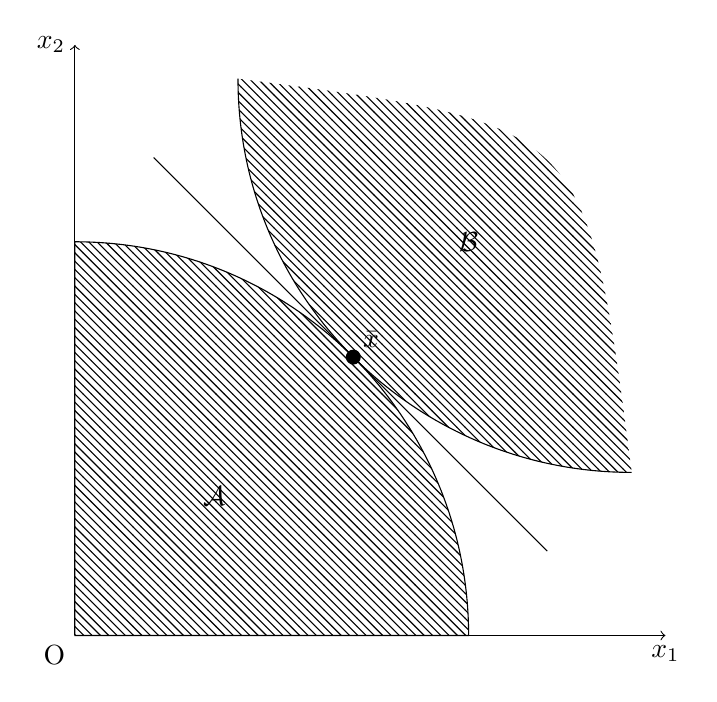
\begin{tikzpicture}[scale=5]
    % 绘制坐标轴
    \draw[->] (0,0) -- (1.5,0) node[below] {$x_1$};
    \draw[->] (0,0) -- (0,1.5) node[left] {$x_2$};
    \draw[black] (0,0) node[below left] {O};

%\draw[domain=0:1, smooth, variable=\x, black] plot ({\x},{ sqrt(1 - \x * \x) })  ;
%\draw[domain={sqrt(2)-1}:sqrt(2), smooth, variable=\x, black] plot ({\x},{ sqrt(2) - sqrt(-\x*\x + 2*sqrt(2)*\x -1   )  } )  ;

\draw (0,0) -- (1,0) arc (0:90:1) -- cycle;
\fill[pattern = north west lines] (0,0) -- ++(0:1) arc (0:90:1) -- cycle;

\draw[domain=0.2:1.2, smooth, variable=\x, black] plot ({\x},{ sqrt(2) - \x  })  ;

\draw ({sqrt(2)} , {sqrt(2)} )  ({sqrt(2) -1}, {sqrt(2)} ) arc (180:270:1)   ;
\fill[pattern = north west lines]  ({sqrt(2)} , {sqrt(2)} )  ({sqrt(2) -1}, {sqrt(2)} ) arc (180:270:1) ({sqrt(2) -1}, {sqrt(2)}) .. controls (1.3,1.3) .. ({sqrt(2) }, {sqrt(2) -1})  ;

\filldraw [black] ({1/sqrt(2)},{1/sqrt(2)}) circle (0.5pt) node[above right] {$\bar{x}$} ;
\filldraw [black] ({1/sqrt(8)},{1/sqrt(8)}) circle node[ ] {$\mathcal{A}$} ;
\filldraw [black] (1, 1) circle node[ ] {$\mathcal{B}$} ;

\end{tikzpicture}
\caption{Separation by the common tangent} %最终文档中希望显示的图片标题
\label{Fig6.1} %用于文内引用的标签
\end{figure}

The two curves meet tangentially at $\bar{x}$, and the figure shows their common tangent line at this point. The curvatures are chosen to ensure a maximum. In Chapter 2 the curvatures were said to reflect diminishing marginal rates of substitution and transformation; now I offer a somewhat different interpretation.

Note that the sets $\mathcal{B}$ and $\mathcal{A}$ lie one to each side of their  common tangent, with only their common point $\bar{x}$ on that line. In other words, the common tangent \textit{separates} the $x$-plane into two halves, each containing one of the sets. In higher dimensions, the common tangent will be a hyperplane; it will likewise separate the two contour sets.

This separation is the crucial property that allows us to distinguish maxima from minima, and obtain sufficient conditions for the maximization problem. Now we must make explicit the hidden conditions on the function $F$ and $G$ that ensure the right curvature.

\section*{Convex Sets and Functions}

Each of the contour sets in Figure \ref{Fig6.1} bulges outward. That is why each bends away from the common tangent at $\bar{x}$, and cannot bend back to meet the other set once again. This property of bulging outward is called convexity. A geometric test of convexity is that given any two points of the set, the whole line segment joining them should lie in the set. Algebraically, a set $S$ of points in $n$-dimensional space is called \textit{convex} if, given any two points $x^a=( x_1^a, x_2^a, \dots, x_n^a)$ and $x^b=( x_1^b, x_2^b, \dots, x_n^b)$ in $S$ and any real number $\theta$ in the closed interval [0,1], the point $[  \theta x^a + (1-\theta)x^b ]$, or
\begin{equation*}
[\theta x_1^a +(1-\theta)x_1^b, \theta x_2^a +(1-\theta)x_2^b, \dots, \theta x_n^a +(1-\theta)x_n^b, ]
\end{equation*}
when written out explicitly in terms of the components, is also in $S$.

Applied to the lower contour set of $G$, this means that if $x^a$ and $x^b$ satisfy the constraint, so does $\theta x^a + (1-\theta)x^b$. In economic applications, constraints often reflect limited availability of resources. Thus $G(x)$ might be the amount of labor necessary to produce the vector $x$, and $c$ the amount of labor available. In such a context, the convexity of the set $G(x) \leq c$ means that a weighted average of two production plans does not need more labor than one of the extremes. This rules out significant economics of scale or specialization. Similarly, applied to the upper contour set of $F$, convexity means that a weighted average of two consumption plans is at least as good as one of the extremes; this assumes a taste for diversity.

Algebraically, the condition states that
\begin{equation*}
G(x^a) \leq c \quad \mbox{and} \quad G(x^b) \leq c \quad \mbox{imply} \quad  G[\theta x^a + (1-\theta) x^b)  ] \leq c  
\end{equation*}
The most severe test of this arises when one of the extreme values equals $c$, therefore we can state the condition alternatively as 
\begin{equation} \label{equa6.1}
 G[\theta x^a + (1-\theta) x^b)  ] \leq \max [G(x^a), G(x^b)]
\end{equation}
for all $x^a$, $x^b$ and for all $\theta \in [0,1]$. An added advantage of this form is that it does not involve the particular number $c$. Since in practice we will have to solve the maximization problem for a general value of $c$, we will need to invoke the condition for all $c$, and a general statement like (\ref{equa6.1}) is the best way to do so.

A function $G$ satisfying (\ref{equa6.1}) is said to be \textit{quasi-convex}. The parallel condition on $F$ will be 
\begin{equation} \label{equa6.2}
 F[\theta x^a + (1-\theta) x^b)  ] \geq \min [F(x^a), F(x^b)]
\end{equation}
for all $x^a$, $x^b$ and for all $\theta \in [0,1]$. Such a function will be called \textit{quasi-concave}.

The \textit{quasi} in the above definitions serves to distinguish them from somewhat stronger properties that often arise in optimization problems. In the usual economic interpretation, quasi-convexity corresponds to a diminishing marginal rate of transformation along the constraint curve, while convexity of the constraint function corresponds to diminishing returns to scale. Similarly, quasi-concavity of the objective function means a diminishing marginal rate of substitution along an indifference curve, while concavity is diminishing marginal utility.

Formally, we define $G$ to be convex if 
\begin{equation} \label{equa6.3}
 G[\theta x^a + (1-\theta) x^b)  ] \leq \theta G(x^a) + (1-\theta) G(x^b)  
\end{equation}
for all $x^a$, $x^b$ and for all $\theta \in [0,1]$. The right-hand side of (\ref{equa6.3}) is obviously no larger than that of (\ref{equa6.1}):
\begin{equation*}  
\begin{array}{rl}
 \theta G(x^a) + (1-\theta) G(x^b) \\ 
\leq &  \theta \max [G(x^a), G(x^b)] + (1-\theta) \max [G(x^a), G(x^b)] \\
\leq & \max [G(x^a), G(x^b)]
\end{array}
\end{equation*}
Therefore if (\ref{equa6.3}) holds, so does (\ref{equa6.1}). In other words, a convex function is quasi-convex; convexity is the stronger property of the two.

Similarly, we define $F$ to be concave if 
\begin{equation} \label{equa6.4}
 F[\theta x^a + (1-\theta) x^b)  ] \geq \theta F(x^a) + (1-\theta) F(x^b)  
\end{equation}
for all $x^a$ , $x^b$ and for all $\theta \in [0,1]$. In words, the graph of the function lies on or above the chord joining any two points of it. Figure \ref{Fig6.2} illustrates this for the case where $x$ is a scalar. It is easy to verify that (\ref{equa6.4}) implies (\ref{equa6.2}): a concave function is also quasi-concave.
\begin{figure}[!htb] %H为当前位置,!htb为忽略美学标准,htbp为浮动图形
\centering %图片居中
%\includegraphics[width=0.8\textwidth]{./Fig3.1.png} %插入图片,[]中设置图片大小,{}中是图片文件名
\begin{tikzpicture}[scale=6]
    % 绘制坐标轴
    \draw[->] (0,0) -- (1.4,0) node[below] {$x$};
    \draw[->] (0,0) -- (0,1.3) node[left] {$v$};
    \draw[black] (0,0) node[below left] {O};

\draw[domain=0.09:1.21, smooth, variable=\x, black] plot ({\x},{ sqrt(  \x  ) })  ;
\draw[domain=0.25:1, smooth, variable=\x, blue] plot ({\x},{  2/3 * \x + 1/3  })  ;
\draw[domain=0.1:0.9, smooth, variable=\x, red] plot ({\x},{    \x + 1/4  })  ;

\filldraw [black] ( 0.25,0.5) circle (0.5pt) node[below right] {$(x^a, F(x^a))$} ;
\filldraw [black] (1, 1) circle (0.5pt) node[below right] {$(x^b, F(x^b))$} ;
\filldraw [blue] (0.6, 0.73) circle  node[below right] {chord} ;
\filldraw [red] (0.9, 1.15) circle  node[above] {tangent} ;
\filldraw [black] ( 1.21,1.1) circle node[right ] {$F(x)$} ;
\filldraw [black] ( 1,0.2) circle node[ ] {$\mathcal{F}$} ;

 \end{tikzpicture}
\caption{Concave function} %最终文档中希望显示的图片标题
\label{Fig6.2} %用于文内引用的标签
\end{figure}

Note that the inequalities in (\ref{equa6.3}) and (\ref{equa6.4}) are weak. Therefore convex and concave functions are allowed to have straight-line segments in their graphs, where the chord coincides with the graph. In particular, a linear function is simultaneously convex and concave. Later we will have occasion to strengthen the concepts of convexity and concavity.

An alternative definition of a concave function is sometimes useful. Consider the $(n+1)$-dimensional space consisting of points like $(x,v)$ where $x$ is an $n$-dimensional vector and $v$ is a scalar. In this, define the set
\begin{equation*}  
  \mathcal{F} = \{  (x,v) | v \leq F(x)   \}
\end{equation*}
Then $F$ is a concave function if and only if $\mathcal{F}$ is a convex set; check this using ({\ref{equa6.4}}). In other words, a concave function traps a convex set underneath its graph. This is easy to see from Figure \ref{Fig6.2}. Similar properties of convex functions are equally easy to state, so I shall leave them to the reader. Finally, if the functions are differentiable, the properties of concavity, quasi-concavity etc. can be expressed in terms of first- and second-order derivatives; I shall do this in Chapter 7.

I must define two more concepts to be able to state the basic mathematical result I need. A point $x^o \in S $ is called an \textit{interior} point if it is surrounded for some distance by points of the set, that is, if there is number $r>0$ such that all points $x$ within distance $r$ of $x^o$ are in $S$. In the plane, such points will form a disc of radius $r$ and centre $x^o$. Then, a point that is interior neither to $S$ nor to the rest of the space is called a \textit{boundary} point of $S$. Thus $x^o$ is a boundary point of $S$ if, for any $r>0$, we can find points in $S$ as well as points not in $S$ within distance $r$ of $x^o$.

In Figure 5.1, for example, $\bar{x}$ is a boundary point of $\mathcal{B}$ and also a boundary point of $\mathcal{A}$. Any $x$ for which $F(x)>\bar{v}$ is an interior point of $\mathcal{B}$ so long as $F$ is continuous. Similarly any point $x$ with $G(x) < c$ is an interior point of $\mathcal{A}$ so long as $G$ is continuous.

The two sets have only the boundary point $\bar{x}$ in common, and the common tangent separates them. Let the equation of this tangent be 
\begin{equation*}
 px \equiv p_1 x_1 + p_2 x_2 = b
\end{equation*}
where $p$ is a row vector of the coefficients, so $px$ is the inner product, or the sum of products of corresponding components, of $p$ and $x$. Of course $p \neq 0$, that is, at least one of $p_1$ and $p_2$ must be non-zero. Since $\bar{x}$ lies on the separating line, we have
\begin{equation*}
 p\bar{x} \equiv p_1 \bar{x}_1 + p_2 \bar{x}_2 = b
\end{equation*}
For all points $x$ to one side of the line, $px$ is greater than $b$, and for all those on the other side, it is less.

If the sets had no points in common at all, there would be a clear gap between them, although it need not be a tangent to either set. But if the sets had interior points in common, then any line entirely above the set $\mathcal{A}$ would have to cut into the set $\mathcal{B}$, and any line entirely below $\mathcal{B}$ would have to cut into $\mathcal{A}$; separation would be impossible.

Convexity of the sets is also important; Figure \ref{Fig6.3} shows two cases, in each of which one of the sets is not convex. The common tangent cuts into the non-convex set, and separation fails.

\begin{figure}[!htp]  % 常见htbp  here top bottom p表示浮动  !表示忽略“美学”标准
 \centering
   \begin{minipage}{1.0\linewidth}
\centering
        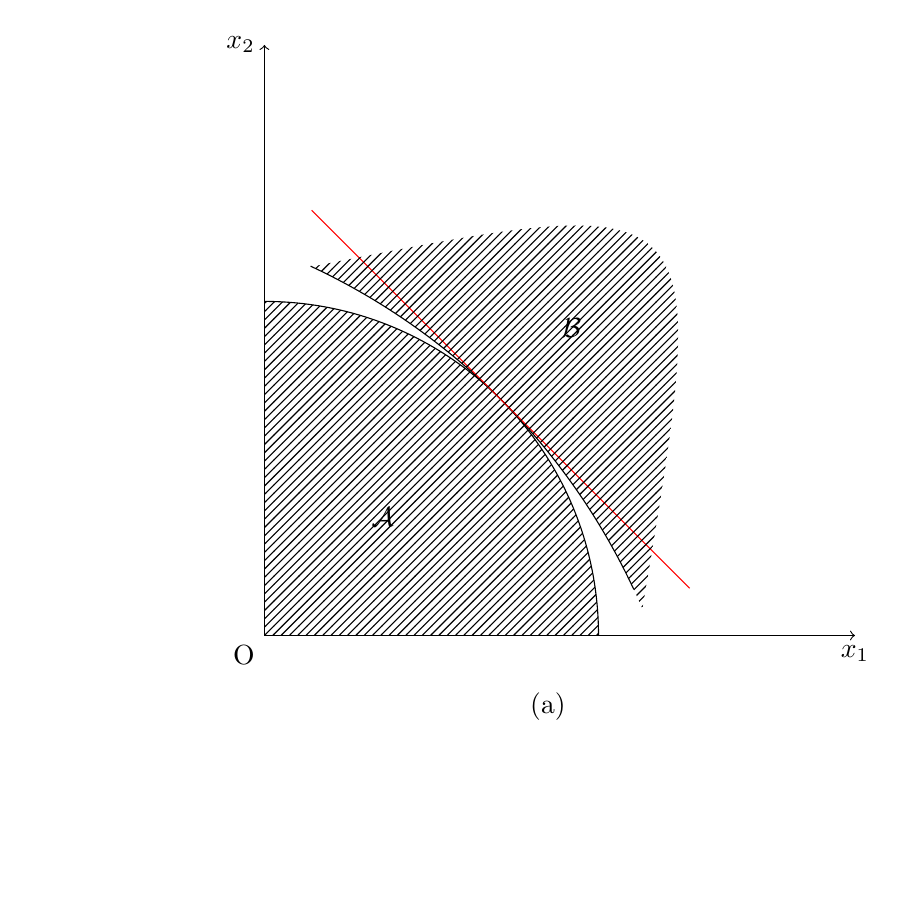
\begin{tikzpicture}[scale=3]
    % 绘制坐标轴
    \draw[->] (0,0) -- (2.5,0) node[below] {$x_1$};
    \draw[->] (0,0) -- (0,2.5) node[left] {$x_2$};
    \draw[black] (0,0) node[below left] {O};

    \coordinate (center1) at (0,0); % 第一个圆弧的圆心
    \def\radius1{{sqrt(2)}} % 第一个圆弧的半径
    \draw (center1) ++(0:\radius1) arc (0:90:\radius1);
    \fill[pattern=north east lines] (0,0) -- (\radius1,0) arc (0:90:\radius1) -- cycle;

    \coordinate (center2) at (-1,-1); % 第二个圆弧的圆心
    \def\radius2{{sqrt(2) *2 }} % 第二个圆弧的半径
    \draw (center2) ++(25:\radius2) arc (25:65:\radius2);

 \draw[domain=0.2:1.8,smooth,red,variable=\x] plot ({\x},{(  2 - \x )}) ;

\fill[pattern=north east lines]  (center2) ++(25:\radius2) arc (25:65:\radius2) -- (0.2,{sqrt(6.56)-1}) .. controls (1.9,1.9) .. (1.6,{sqrt(1.24)-1})   ;

 %   \draw[domain=0:sqrt(2),smooth,variable=\x] plot ({\x},{( sqrt(2-\x*\x)   )}) ;
 %   \draw[domain=0.2:1.8,smooth,red,variable=\x] plot ({\x},{(  2 - \x )}) ;
 %   \draw[domain=0.2:1.6,smooth,variable=\x] plot ({\x},{( sqrt(7-2*\x-\x*\x) -1   )}) ;

 \draw[black] (0.5,0.5) node[] {$\mathcal{A}$}; 
 \draw[black] (1.3,1.3) node[] {$\mathcal{B}$}; 

\draw[black] (1.2,-0.2 ) node[below] {(a)} ; 
        \end{tikzpicture}
   \end{minipage} 

   \begin{minipage}{1.0\linewidth}
\centering
       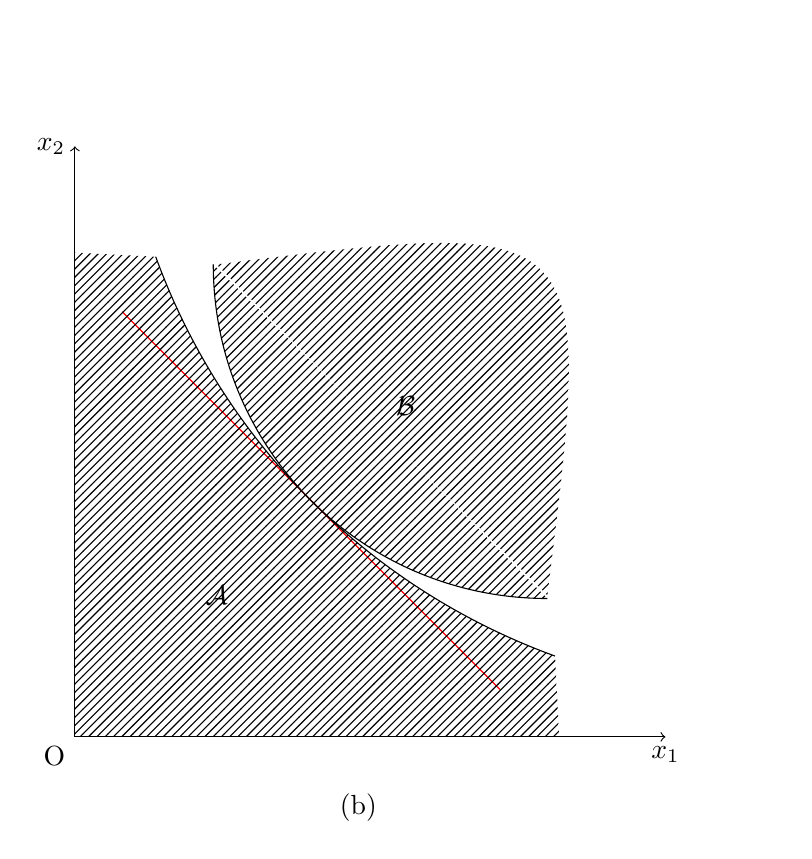
\begin{tikzpicture}[scale=3]
    % 绘制坐标轴
    \draw[->] (0,0) -- (2.5,0) node[below] {$x_1$};
    \draw[->] (0,0) -- (0,2.5) node[left] {$x_2$};
    \draw[black] (0,0) node[below left] {O};

% \draw[domain=0.6:2,smooth,variable=\x] plot ({\x},{( 2-sqrt(- \x*\x +4*\x -2) )}) ;
    \coordinate (center1) at (2,2); % 第一个圆弧的圆心
    \def\radius1{{sqrt(2)}} % 第一个圆弧的半径
    \draw (center1) ++(180:\radius1) arc (180:270:\radius1);
\fill[pattern=north east lines]  (center1) ++(180:\radius1) arc (180:270:\radius1) -- (0.6,2) .. controls (2.2,2.2) .. (2,0.6)   ;
    
\draw[domain=0.2:1.8,smooth,red,variable=\x] plot ({\x},{(  2-  \x )}) ;

% \draw[domain=0.4:2,smooth,variable=\x] plot ({\x},{( 3-sqrt(- \x*\x +6*\x -1) )}) ;
    \coordinate (center2) at (3,3); % 第一个圆弧的圆心
    \def\radius2{{2*sqrt(2)}} % 第一个圆弧的半径
    \draw (center2) ++(200:\radius2) arc (200:250:\radius2);
\fill[pattern=north east lines]  (center2) ++(200:\radius2) arc (200:250:\radius2)  -- (2.05,0) -- (0,0) -- (0,2.05);

 \draw[black] (0.6,0.6) node[] {$\mathcal{A}$}; 
 \draw[black] (1.4,1.4) node[] {$\mathcal{B}$}; 

\draw[black] (1.2,-0.2 ) node[below] {(b)} ; 
      \end{tikzpicture}
   \end{minipage} 
 \caption{Partial failure of decentralization} \label{Fig6.3} 
\end{figure}

All these ideas are formalized in the following theorem. I hope most readers will find the pictorial argument convincing, and so shall not give a formal proof. I shall only state the result in the simplest form that suits my purpose, even though more general results of this kind are available.

\textit{Separation Theorem:} If $\mathcal{B}$ and $\mathcal{A}$ are two convex sets, that have no interior points in common, and at least one of the sets has a non-empty interior, then we can find a non-zero vector $p$ and a number $b$ such that the hyperplane $px=b$ separates the two sets, or 
\begin{equation} \label{equa6.5}
 px  \left\{  \begin{array}{ll}  
\leq b &  \mbox{for all} \  x \in \mathcal{A} \\
\geq b &  \mbox{for all} \  x \in \mathcal{B}
\end{array}
  \right.
\end{equation}
 
The qualification that at least one of the sets should have a non-empty interior rules out some awkward cases where the sets are of smaller dimension than the whole space. I state it for completeness, but in our economic applications the contour set of the objective function is full-dimensional, so no difficulty arises on this account.

\section*{Optimization by Separation}

Let $F$ and $G$ be continuous functions, with $F$ quasi-convex and $G$ quasi-concave. Consider the maximization of $F(x)$ subject to the constraint $G(x) \leq c$. So long as the constraint set is bounded, the problem has a solution. In most economic applications in this book, except in one case of infinite time-horizons in Chapter 10, existence of an optimum is not a problem. Let $\bar{x}$ denote the optimum. All the conditions assumed in Figure 6.1 are met, and the Separation Theorem applies. Let $px=b$ be the equation of the separating common tangent. The equation is unaffected if we multiply it through by -1, but that will reverse the directions of the inequalities in (\ref{equa6.5}). To ensure that the inequalities hold the right way for the sets $\mathcal{B}$ and $\mathcal{A}$ as stated there, we should choose $p_1$ and $p_2$ to be positive.

Since the point $\bar{x}$ lies on the separating tangent, we have $p \bar{x} =b$. Therefore (\ref{equa6.5}) tells us that $\bar{x}$ gives the largest value of $px$ among all points in $\mathcal{A}$, that is, among all points satisfying $G(x) \leq c$. Similarly, $\bar{x}$ gives the smallest value of $px$ among all points in $\mathcal{B}$, that is, among all points satisfying $F(x) \geq \bar{v}$. This is the basic result of this section.

\textit{Optimization by Separation:} Given a quasi-concave function $F$ and a quasi-convex function $G$, the point $\bar{x}$ maximizes $F(x)$ subject to the constraint $G(x) \leq c$ if, and only if, there is a non-zero vector $p$ such that
\begin{itemize}
\item (i) $\bar{x}$ maximizes $px$ subject to $G(x) \leq c$, and
\item (ii) $\bar{x}$ minimizes $px$ subject to $F(x) \geq \bar{v}$.
\end{itemize}

The generalization to several constraints is straightforward. The set $\mathcal{B}_i$ of points for which $G^i(x) \leq c_i$ is convex if $G^i$ is quasi-convex. If this is so for all $i$, then the set $\mathcal{B}$ of points satisfying all the constraints, being the intersection of the convex sets $\mathcal{A}_i$, is itself convex; this is easy to verify using the definition of a convex set. Then the argument proceeds as above.

Note the `if and only if' in the statement of the result. The stated conditions are both necessary and sufficient for optimality: if $\bar{x}$ is optimal, the conditions will hold, and vice versa. In both respects, the result goes beyond the Lagrange or Kuhn-Tucker conditions we met before. This is the first time we have met a sufficient condition, therefore it is of interest in itself. But the conditions are not easy to verify in practical applications. After all, we have replaced one optimization problem by two, and have given no useful criterion for judging when either one of them is solved. In the next two chapters we shall see sufficient conditions that are more useful in this regard.

The real benefit from splitting the maximization problem into two separate problems, in each of which the objective function is linear, comes from its economic interpretation. It raises the possibility of \textit{decentralizing} optimal resource allocations using prices. To give the simplest interpretation, suppose $x$ is the production cum-consumption vector, the constraints reflect limited resource availability, and the objective is the utility function. Now interpret $p$ as the row vector of prices of outputs. Then part (i) of the above theorem says that the optimum $\bar{x}$ would be produced by an entrepreneur seeking the maximum value of output, and (ii) says that $\bar{x}$ would also be demanded by a consumer trying to reach the target utility level $\bar{v}$ in the least cost manner. If we assume away some technical complications that arise when there are free goods, this is equivalent to maximizing utility subject to the budget constraint $px \leq p \bar{x}$. Thus the original problem of social optimization can be decentralized. Let an entrepreneur choose the production plan. The resulting value of output accrues to the consumer in the usual circular flow of income. Then let the consumer solve his own utility maximization problem. This separation of decisions has two advantages. One is informational: the producer need know nothing about the consumer's tastes, and the consumer need know nothing about the production technology. For each, the relevant information about the other is adequately summarized in the price vector $p$. The other advantage relates to incentives: the process relies on the self-interest of each side to ensure the effective implementation of the optimum.

Note that nothing of economic substance will change if we multiply the vector $p$ and the related number $b$ by the same positive number. Another way of saying the same thing is that only relative prices like ($p_1/ p_2$) matter for economic decisions. The separate maximization problems in the above theorem are solved when producers equate their marginal rates of substitution, and consumers their marginal rates of transformation, to the relative prices.

Of course decentralization in practice is more complicated. When there are several producers and consumers, issues of external effects and income distribution must be addressed. There is also the question of how the correct price vector is found. All too often, people do not have the incentive to reveal their private information that is needed to calculate the right prices, taxes etc. Their behavior imposes additional constraints on the social of optimization problem. Such issues are discussed at length in microeconomics textbooks, and continue to be the subject of active research. But the simple story above remains a useful starting point.

If we do not assume both $\mathcal{B}$ and $\mathcal{A}$ ti be convex, full decentralization is not possible. Figure \ref{Fig6.3} illustrates this. In case (a), $\mathcal{B}$ is not convex and $\bar{x}$ does not minimize $px$ over it. In case (b), $\mathcal{A}$ is not convex and $\bar{x}$ does not maximize $px$ over it. Here the production technology has economies of scale or of specialization. But in both cases, $\bar{x}$ does maximize $F(x)$ subject to $G(x) \leq c$. Thus the theorem on Optimization by Separation, which started out by assuming that $F$ to be quasi-concave and $G$ quasi-convex, does not cover all economically interesting cases. What really matters is the \textit{relative} curvature of the contours of $F$ and $G$. In Chapter 8 I shall develop conditions that capture this idea using calculus.

\section*{Uniqueness}

In figure 6.1 the boundaries of the two sets $\mathcal{B}$ and $\mathcal{A}$ were shown as smooth curves. But this is not necessary according to the definition of a convex set. In general, a convex set can have straight-line segments along its boundary; this will still permit the whole line segment joining any two points of the set to lie in the set. There can also be kinks along the boundary so long as the corners point outward.

These possibilities have implications for separation and optimization. Figure \ref{Fig6.4} illustrates some such cases. In (a), two corners happen to meet at the optimum $\bar{x}$. Now we can find many lines through $\bar{x}$ which separate the two sets, that is, the decentralizing price vector $p$ is not unique. None of the possible separating lines can be called a tangent in the usual sense, but that is not essential for the economics of the problem. Decentralization depends only on the separation property, namely that the two sets lie one on each side of the line $px=b$. Thus separation is a more general notion than that of a common tangent. This generalization, and the decentralization property, hold even when the functions $F$ and $G$ fail to have derivatives. In such cases the usual smooth marginal rates of substitution and transformation are not defined, and cannot be equated to price ratios in the usual way. What happens is that there are different marginal rates of substitution to the left and the right of a kink in an indifference curve, and the price ratio lies between the two. Similarly for transformation curves.

\begin{figure}[!htp]  % 常见htbp  here top bottom p表示浮动  !表示忽略“美学”标准
 \centering
 \subfloat[ ] %第一张子图
 {
   \begin{minipage}{0.5\linewidth}
\centering
        \begin{tikzpicture}[scale=2]
    % 绘制坐标轴
    \draw[->] (0,0) -- (2.5,0) node[below] {$x_1$};
    \draw[->] (0,0) -- (0,2.5) node[left] {$x_2$};
    \draw[black] (0,0) node[below left] {O};

    \draw[domain=0:1,smooth,variable=\x] plot ({\x},{(   -0.2 * \x +1.2)}) ;
    \draw[domain=1:1.8,smooth,variable=\x] plot ({\x},{(   -0.8 * \x +1.8)}) ;
    \draw[domain=1:1.25,smooth,variable=\x] plot ({\x},{(   -4 * \x +5)}) ;
    \draw[domain=0.4:1,smooth,variable=\x] plot ({\x},{(   -1.7 * \x +2.7)}) ;

 \draw[black] (0.5,0.5) node[] {$\mathcal{A}$}; 
 \draw[black] (1.5,1.5) node[] {$\mathcal{B}$}; 
        \end{tikzpicture}
   \end{minipage} }
 \subfloat[ ] %第二张子图
   {
   \begin{minipage}{0.5\linewidth}
\centering
       \begin{tikzpicture}[scale=2]
    % 绘制坐标轴
    \draw[->] (0,0) -- (2.5,0) node[below] {$x_1$};
    \draw[->] (0,0) -- (0,2.5) node[left] {$x_2$};
    \draw[black] (0,0) node[below left] {O};

    \draw[domain=0.3:1.2,smooth,variable=\x] plot ({\x},{( -1 * \x +1.5)}) ;
    \draw[] (0,1.3) -- (0.3,1.2) ; 
    \draw[] (1.2,0.3) -- (1.3,0) ; 
    \draw[] (0.5,1 ) -- (0.2,2) ; 
    \draw[] (1,0.5) -- (2,0.4) ; 
 \draw[black] (0.4,0.4) node[] {$\mathcal{A}$}; 
 \draw[black] (1.3,1.3) node[] {$\mathcal{B}$}; 
      \end{tikzpicture}
   \end{minipage} }

 \centering
 \subfloat[ ] %第三张子图
 {
   \begin{minipage}{0.5\linewidth}
\centering
        \begin{tikzpicture}[scale=2]
    % 绘制坐标轴
    \draw[->] (0,0) -- (2.5,0) node[below] {$x_1$};
    \draw[->] (0,0) -- (0,2.5) node[left] {$x_2$};
    \draw[black] (0,0) node[below left] {O};

    \draw[domain=1:1.8,smooth,variable=\x] plot ({\x},{(0.5+ 0.5* (\x -2) * (\x -2))}) ;
    \draw[domain=0.5:1 ,smooth,variable=\x] plot ({\x},{(2 - 4* (\x -0.5)  *  (\x -0.5) )}) ;
    \draw[] (1,0) -- (1,2) ; 
 \draw[black] (0.5,0.5) node[] {$\mathcal{A}$}; 
 \draw[black] (1.5,1.5) node[] {$\mathcal{B}$}; 
        \end{tikzpicture}
   \end{minipage} }
 \subfloat[ ] %第四张子图
   {
   \begin{minipage}{0.5\linewidth}
\centering
       \begin{tikzpicture}[scale=2]
    % 绘制坐标轴
    \draw[->] (0,0) -- (2.5,0) node[below] {$x_1$};
    \draw[->] (0,0) -- (0,2.5) node[left] {$x_2$};
    \draw[black] (0,0) node[below left] {O};

    \draw[domain=0.2:1,smooth,variable=\x] plot ({\x},{( -0.6 * \x  +1.6)}) ;
    \draw[domain=1:1.7,smooth,variable=\x] plot ({\x},{( -0.2 * \x  +1.2)}) ;
    \draw[domain=0.5:1.5 ,smooth,red,variable=\x] plot ({\x},{(2 - \x)}) ;
    \draw[] (1,0) -- (1,2) ; 
 \draw[black] (0.5,0.5) node[] {$\mathcal{A}$}; 
 \draw[black] (1.5,1.5) node[] {$\mathcal{B}$}; 
      \end{tikzpicture}
   \end{minipage} }
 \caption{Optima at kinks and along flats} \label{Fig6.4} 
\end{figure}

In case (b), the two sets have a flat portion in common. Now any point along this region serves as the optimum $\bar{x}$. All such points yield the same value of the objective function $F(x)$, so the non-uniqueness is not a cause for concern. There is, however, a problem about decentralization. Given $p$, all points on the flat portion of $\mathcal{A}$ will yield the same value of output to the producer, and all those on the flat portion of $\mathcal{B}$ will yield equal utility to the consumer. Their choices will be arbitrary to that extent, and there is no reason why the independent choices should coincide. We can only make the weaker claim that \textit{if} the two happen to make coincident choices, neither will have any positive incentive to depart from these choices. This is a standard limitation in any careful statement of economic equilibrium theory.

If the two boundaries have vertical parts in common, as in case (c), we have a vertical separating line. In its equation, $p_2=0$, and in the decentralization interpretation, good 2 is a free good. Similarly for horizontal separating lines $p_1=0$. In case (d), there is also a kink, and while there is a vertical separating line, there are also non-vertical ones. Thus without stronger assumptions, it is not possible to guarantee strictly positive prices. In fact, if the boundaries sloped upward at the optimum, the common tangent would have a positive slope and one of the prices would be negative. This is usually avoided by assuming \textit{either} that there is free disposability of both goods, when the boundary of $\mathcal{A}$ cannot slope upward, \textit{or} that both goods are desirable, when the boundary of $\mathcal{B}$ cannot slope upward. Both these assumptions have been implicit in all the illustrative figures.

To sum up, problems of kinks are not serious; in fact they allow us to generalize the concept of tangency and preserve the decentralization property. Problems of flats are more serious because optimum choices can be non-unique and it might be difficult to get all producers and consumers to make mutually consistent choices. Therefore it is useful to know what property of the function $F$ and $G$ removes this difficulty. A strengthening of the concepts of quasi-concavity and quasi-convexity is needed.

Recall that definition of a convex set: $S$ is convex if, given two points $x^a$ and $x^b$ in $S$, and any $\theta$ satisfying $0 \leq \theta \leq 1$, the intermediate point $\theta x^a + (1-\theta)x^b$ is also in $S$. The whole line segment joining $x^a$ to $x^b$ could lie along the boundary of $S$; that is how the boundary could have flat portions. We could strengthen the definition by requiring that all points of the line segment except the end-points are interior points: whenever $x^a$ and $x^b$ are distinct and $\theta$ is not equal to 0 or 1, the point $\theta x^a + (1-\theta)x^b$  should be interior to $S$. If this is so, the set $S$ is called strongly convex. The function $F$ is called \textit{strictly quasi-concave} if all of its upper contour sets are strongly convex.

Now consider the problem of maximizing $F(x)$ subject to $G(x) \leq c$, where $F$ is strictly quasi-concave and $G$ is quasi-convex. Suppose $\bar{x}$ satisfies the conditions of the theorem of Optimization by Separation. Then is is the unique solution to the optimization problem.

To see this, suppose $\hat{x}$ is another solution. Both must be feasible for the second (or consumer's) half of the pair of decentralized optimization problem. Thus
\begin{equation*}
p \bar{x} = p \hat{x} =b  \quad \mbox{and} \quad F(\bar{x}) = F(\hat{x})  = \bar{v}
\end{equation*}
Take the midpoint $\tilde{x} = \frac{1}{2} (\bar{x} + \hat{x})$. Since $F$ is strictly quasi-concave, this is an interior point of the upper contour set $\mathcal{B}$, that is, $F(\tilde{x}) > v$. Then we can find a neighboring point that is still in $\mathcal{B}$, and has a smaller value of $px$ than $\bar{x}$. To be formal, take $\epsilon$ positive, and define $x^\prime$ by
\begin{equation*}
 x^{\prime}_j = \tilde{x}_j - \epsilon p_j \quad \mbox{for} \  j=1,2,\dots,n
\end{equation*}
Because $\tilde{x}$ is an interior point of $\mathcal{B}$, for $\epsilon$ small enough, $x^\prime$ is in $\mathcal{B}$. And 
\begin{equation*}
\begin{array}{rl}
p x^\prime & = p \tilde{x} - \epsilon p^2 \\
   & = \frac{1}{2}(p \bar{x} + p \tilde{x} ) - \epsilon p^2\\
   & = \frac{1}{2}(b+b) - \epsilon p^2 \\
   & < b
\end{array} 
\end{equation*}
where $p^2$ denotes the inner product of the vector $p$ with itself, namely $\sum_j p_j^2 > 0$. Thus we have found a point $x \in \mathcal{B}$ with $px <b$, contradicting the separation property. This contradiction stems from the initial supposition that $\bar{x}$ was not unique. Therefore that supposition must be wrong. Thus strict quasi-concavity of $F$ implies the uniqueness of the maximizer.

Strict quasi-convexity of $G$ would do equally well. When there are several constraints, we have to assume every component constraint function $G^i$ to be strictly quasi-convex to ensure strong convexity of the constraint set $\mathcal{A}$.

\section*{Examples}

\subsubsection*{\textit{Example 6.1: Illustration of Separation}}

Suppose there are two non-negative choice variables labeled $x$ and $y$, and the functions $F$ and $G$ are given by 
\begin{equation*}
F(x,y) = xy \quad \mbox{and} \quad G(x,y) = x^2 + y^2
\end{equation*}
The constraint is $G(x,y ) \leq 25$

Figure \ref{Fig6.5} illustrates this. The feasible set $\mathcal{A}$ consists of the quarter-circle and all points below it; boundaries of the upper contour sets of $F$ for various values $v$ are shown as a family of rectangular hyperbolas. The optimum occurs at $(x,y) = (5/\sqrt{2},  5/\sqrt{2})$, and the maximized value of $F(x,y)$ is $\bar{v}= 12 \frac{1}{2}$.
\begin{figure}[!htb] %H为当前位置,!htb为忽略美学标准,htbp为浮动图形
\centering %图片居中
%\includegraphics[width=0.8\textwidth]{./Fig3.1.png} %插入图片,[]中设置图片大小,{}中是图片文件名
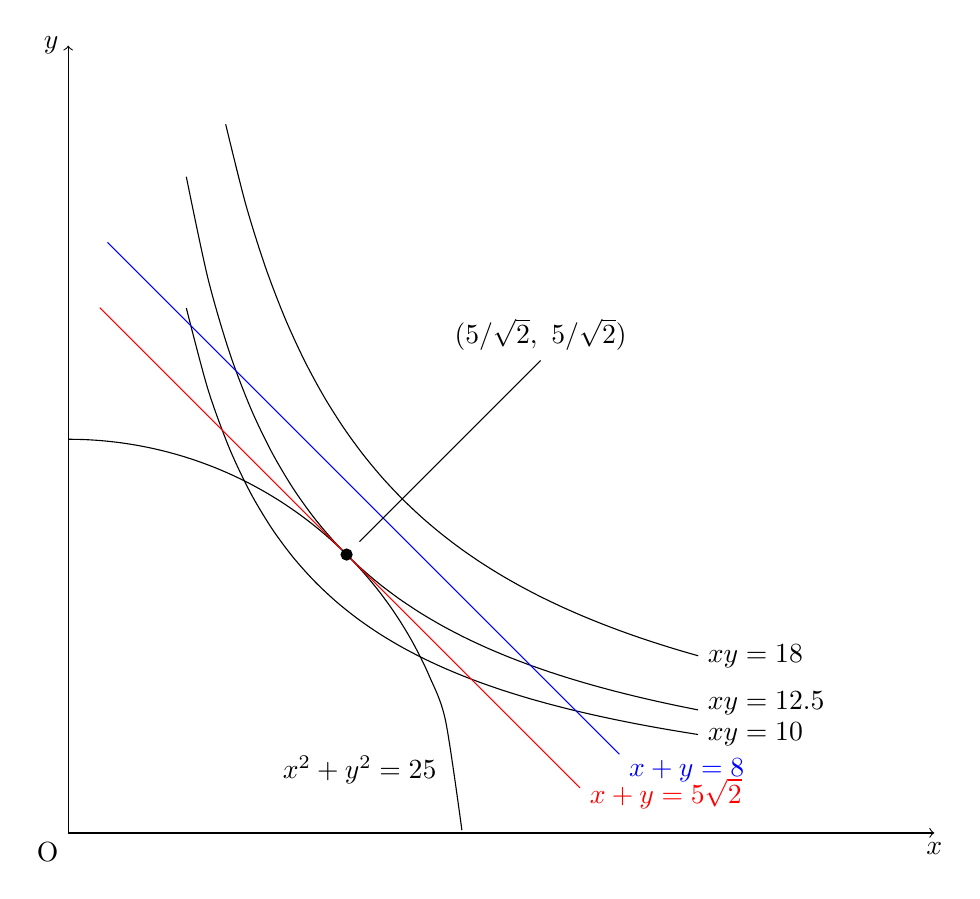
\begin{tikzpicture}[scale=1]
    % 绘制坐标轴
    \draw[->] (0,0) -- (11,0) node[below] {$x$};
    \draw[->] (0,0) -- (0,10) node[left] {$y$};
    \draw[black] (0,0) node[below left] {O};

\draw[domain=0 :5, smooth, variable=\x, black] plot ({\x},{ sqrt( 25 - \x *\x ) })  ;
\draw[domain=1.5:8, smooth, variable=\x, black] plot ({\x},{   12.5 / \x   })  ;
\draw[domain=2:8, smooth, variable=\x, black] plot ({\x},{   18 / \x   })  ;
\draw[domain=1.5:8, smooth, variable=\x, black] plot ({\x},{   10 / \x   })  ;
\draw[domain=0.5:7, smooth, variable=\x, blue] plot ({\x},{  8- \x   })  ;
\draw[domain=0.4:6.5, smooth, variable=\x, red] plot ({\x},{  5*sqrt(2) - \x   })  ;

\filldraw [black] ( 8,9/4) circle  node[ right] {$xy=18$} ;
\filldraw [black] (8,1.65) circle   node[ right] {$xy=12.5$} ;
\filldraw [black] (8, 5/4) circle   node[ right] {$xy=10$} ;
\filldraw [blue] (7, 0.8) circle   node[ right] {$x+y=8$} ;
\filldraw [red] (6.5, 0.5) circle   node[ right] {$x+y=5 \sqrt{2}$} ;
\filldraw [black] ({5/sqrt(2)}, {5/sqrt(2)}) circle (2pt)  node[  ] {}  ;
\draw[domain=3.7:6, smooth, variable=\x, black] plot ({\x},{    \x   })  ;
\filldraw [black] ( 6,6) circle  node[ above] {$(  5/\sqrt{2} , \  5/\sqrt{2}  )$} ;
\filldraw [black] ( 4.8,0.5) circle  node[ above left] {$x^2 + y^2=25 $} ;
 \end{tikzpicture}
\caption{Illustration of separation} %最终文档中希望显示的图片标题
\label{Fig6.5} %用于文内引用的标签
\end{figure}

The upper contour set $\mathcal{B}$ corresponding to $\bar{v}$ touches the feasible set at the optimum; they are separated by the common tangent $x+y=5 \sqrt{2}$. The upper contour set of $F$ for the larger value 18 has no points in common with $\mathcal{A}$, and we can draw a separating line $x+y=8$ through the clear gap between them. For a smaller value than $\bar{v}$, say 10, the upper contour set of $F$ and the feasible set have interior points in common ( the lens-shaped area of their intersection), and the two cannot be separated.

\subsubsection*{\textit{Example 6.2: Indirect Utility and Expenditure Functions}}

A utility maximizing consumer's indirect utility function and expenditure function were defined in Example 5.2. Here I shall examine their convexity properties.

Begin with the expenditure function
\begin{equation} \label{equa6.6}
E(p,u) = \min\limits_x \{  px \ | \  U(x) \geq u  \}
\end{equation}
This is concave as a function of $p$ for each fixed $u$. To see this, take any two price vectors $p^a$ and $p^b$, and any number $\theta$ in [0,1]. Let $p^c = \theta p^a + (1-\theta)p^b$. Then we need to show that
\begin{equation} \label{equa6.7}
E(p^c,u) \geq  \theta E(p^a, u) + (1-\theta) E(p^b,u)
\end{equation}

Let $x^c$ achieve the expenditure minimization for $p^c$. Of course $x^c$ must satisfy the constraint, so $U(x^c) \geq u$. The constraint does not involve the price vectors, so $x^c$ is also feasible when the price vector is $p^a$ of $p^b$. In each case it cannot achieve a smaller expenditure than the minimum:
\begin{equation} \label{equa6.8}
p^a x^c \geq E(p^a, u) \quad \mbox{and} \quad p^b x^c \geq E(p^b, u) 
\end{equation}
Multiply the first of these by $\theta$ and the second by ($1-\theta$); this leaves the directions of the inequalities unchanged since both multipliers are non-negative. Adding the two,
\begin{equation*}  
p^c x^c = [ \theta p^a + (1-\theta)p^b ]  x^c \geq \theta E(p^a, u) + (1-\theta)  E(p^b, u)
\end{equation*}
The left-hand side is just $E(p^c, u)$. This proves (\ref{equa6.7}).

The economic intuition is that as the price vector changes, one \textit{could} leave the quantity vector unchanged. Then the expenditure would change linearly with the price. To the extent that there is substitution along the indifference curves, the quantity choice can be adapted to the changing prices. This will change the expenditure slower than linearly, that is, the minimized expenditure will be a concave function of prices. Another way of looking at this is to examine the worst case, when there is \textit{no} substitution in consumption. The indifference curves are L-shaped, and $x^c$ is the optimal way of achieving the utility level $u$, irrespective of the prices. The two inequalities in (\ref{equa6.8}) hold as equations, and then (\ref{equa6.7}) is an equation, too: expenditure is linear in prices.

Next the indirect utility function,
\begin{equation} \label{equa6.9}
V(p,I) = \max\limits_x \{ U(x) \ | \ px \leq I \}
\end{equation}
This is quasi-convex in ($p,I$). The proof follows a similar line. Let ($p^a, I^a$) and ($p^b, I^b$) be any two price income vectors, and $\theta$ any number in [0,1]. Let
\begin{equation*}  
 (p^c, I^c) = \theta(p^a, I^a) + (1-\theta)(p^b, I^b)
\end{equation*}
and suppose $x^c$ solves the utility-maximization problem for ($p^c, I^c$). It satisfies the constraint, so $p^c x^c \leq I^c$.

Now I claim that $x^c$ is feasible for at least one of the price-income vectors ($p^a, I^a$) and ($p^b, I^b$). For if not, we would have
\begin{equation*}  
 p^a x^c > I^c \quad \mbox{and} \quad p^b x^c > I^c
\end{equation*}
Multiplying the first by $\theta$, the second by ($1-\theta$) and adding, we would get $p^c x^c > I^c$, contradicting the feasibility of $x^c$ for ($p^c, I^c$).

In whichever situation $x^c$ is feasible, its utility $U(x^c)$ cannot exceed the maximum utility achievable in that situation. Therefore at least one of 
\begin{equation*}  
 U(x^c) \leq V(p^a ,I^a) \quad \mbox{and} \quad U(x^c) \leq V(p^b ,I^b)
\end{equation*}
must be true. Then
\begin{equation*}  
 V(p^c ,  I^c) \leq \max [ V(p^a, I^a), V(p^b, I^b)  ]
\end{equation*}
which is just the statement of quasi-convexity of $V$.

In other words, the \textit{lower} contour sets of the indirect utility function are convex. This has an unfortunate 
consequence. When the government chooses indirect taxes optimally, it is in effect choosing prices to maximize an indirect utility function. Our result says that the objective function has the wrong curvature for a maximization problem. Therefore sufficient conditions for optimal tax problems are hard to verify.

\section*{Exercises} 

\subsubsection*{\textit{Exercise 6.1: Commodities that Cause Disutility}}

How is Figure 6.1 altered when (a) one of the choice variables is labor, which gives disutility to consumers and is an input to production, and (b) when one of the goods is pollution, which gives disutility to consumers and is the by-product of an economically desirable good which is the other choice variable? Interpret the associated prices in each of these contexts.

\subsubsection*{\textit{Exercise 6.2: Convexity of a Firm's Profit Function}}

A firm chooses vectors $x$ of inputs and $y$ of outputs subject to a production possibility constraint $G(x,y) \leq 0$, to maximize profit ($qy-px$), where $q$ denotes the row vector of output prices and $p$ that of input prices. Let $\Pi(q,p)$ be the maximized profit expressed as a function of the prices. Prove that $\Pi$ is a convex function of ($q,p$).

\subsubsection*{\textit{Exercise 6.3: Corner Solutions}}

Consider an economy with labor endowment $L$. It can produce two goods $x_1$ and $x_2$. A unit of good $j$ needs a fixed amount $a_j$ units of labor, so the production possibility constraint is 
\begin{equation*}
a_1 x_1 + a_2 x_2 \leq L
\end{equation*}
The world prices of the two goods are $p_1$ and $p_2$, independent of the levels of production chosen by this country. The aim is to maximize the value of national product, ($p_1 x_1 + p_2 x_2$).

Draw a figure and solve the problem by separation of two convex sets. You will need to consider two cases separately, depending on which of ($p_1 / p_2$) and ($a_1 / a_2$) is larger.

Having seen the solution in the figure, verify Lagrange's conditions. Find and interpret the Lagrange multiplier. Show that the maximized national product, expressed as a function of the prices( the revenue function or the GNP function) is 
\begin{equation*}
R(p_1, p_2) = \max (p_1 / a_1, p_2 / a_2)
\end{equation*}
 








\chapter{Concave Programming}

\section*{Concave Functions and Their Derivatives}

In the last chapter I defined convex sets and quasi—concave and concave functions, and developed a geometric approach to constrained optimization based on the separation of two convex sets. This had the conceptual merit of suggesting a decentralized implementation of society's economic optimization problem. But it was of limited value in solving actual examples. In this chapter I combine the idea of convexity with a more conventional calculus approach. The result is that the Lagrange or Kuhn-Tucker conditions, in conjunction with convexity properties of the objective and constraint functions, are sufficient for optimality.

The first step is to express the convexity etc. of functions in terms of their derivatives. In Chapter 6, a concave function was defined by the property that the chord joining any two points on its graph lies entirely below (or at most coincident with) the graph; see Figure \ref{Fig6.2}. If we let the point $x^b$ move closer and closer to $x^a$, the chord approaches the tangent to $F(x)$ at $x^a$. The requirement of concavity then says that the graph of the function should lie on or below the tangent. The worst that is allowed is when $F(x)$ has straight-line segments, then the tangent could coincide with our such segment.

More formally, for $\theta \in [0,1]$, we have
\begin{equation*}
F[x^a + \theta(x^b - x^a)] = F[\theta x^b +(1-\theta)x^a] \geq \theta F(x^b) + (1-\theta) F(x^a)
\end{equation*}
Therefore
\begin{equation*}
   \dfrac{F[x^a + \theta(x^b - x^a)] - F(x^a)}{\theta} \geq  F(x^b) - F(x^a)
\end{equation*}
Now let $\theta$ tend to zero. Provided $F$ is differentiable, the chain rule says that the left-hand side tends to $F_x(x^a)(x^b - x^a)$, where $F_x$ is the row vector of partial derivatives, and the product is an inner product. Then
\begin{equation} \label{equa7.1}
  F_x(x^a)(x^b - x^a) \geq F(x^b) - F(x^a)
\end{equation}
When $x$ is one—dimensional, $F_x(x^a)$ is just the slope of the tangent to $F(x)$ at at $x^a$, so the left-hand side is the vertical distance along this tangent as we move from $x^a$ to $x^b$. Then (\ref{equa7.1}) says that the change in the value of a concave function is overestimated by its tangent, that is, the tangent lies above the curve. More generally, the left-hand side is just the linear term in the Taylor approximation to the change in $F(x)$ using $x^a$ as the initial point; this approximation is an overestimate of the change in $F(x)$.

Similarly, if $G$ is a differentiable convex function, then
\begin{equation} \label{equa7.2}
  G_x(x^a)(x^b - x^a) \leq G(x^b) - G(x^a)
\end{equation}
A particularly important class of optimization problems has a concave objective function and convex constraint functions; the term \textit{concave programming} is often used to describe the general problem of this kind, and it is the subject of the next section.

\section*{Concave Programming}

Consider the maximization of $F(x)$ subject to a vector constraint $G(x) \leq c$, where $F$ is differentiable and concave, and each component constraint function $G^i$ is differentiable and convex. This is called the general problem of \textit{concave programming}. For concreteness and economic interest, I shall use the terminology of the production problem, where $x$ is the vector of outputs, $F(x)$ is the revenue from the sale of the outputs, $c$ a fixed vector of input supplies, and $G(x)$ is the vector of inputs needed to produce $x$. But the mathematics is independent of this interpretation.

The conditions of optimality for a particular value of $c$ are found by first considering the problem for a general $c$. Then the optimum choice of $x$, say $\bar{x}$, and the maximum value $v = F (\bar{x})$, both become functions of $c$. Let $X(c)$ denote the optimum choice
function, and $V(c)$ the maximum value function.

The first result is that $V$ is a non-decreasing function. This is because an $x$ that was feasible for a given value of $c$ remains feasible
when any component of $c$ increases, so the maximum value cannot decrease.

The next result is that $V$ is concave. Let $c$ and $c^\prime$ be any two input supply vectors, with
\begin{equation*}
\bar{x} = X(c), \quad \bar{x}^\prime = X(c^\prime), \quad \bar{v} =V(c), \quad \bar{v}^\prime = V(c^\prime)
\end{equation*}
Since the optimum choices must be feasible, we have $G(\bar{x}) \leq c$ and $G(\bar{x}^\prime) \leq c^\prime$.

Now let $\theta$ be any number in [0,1]. For $V$ to be concave, it should be possible to achieve revenue at least as high as $\theta V(c) + (1-\theta)V(c^\prime)$ when the input supply vector is $\theta c + (1-\theta)c^\prime$. A natural candidate for the output vector is $\theta \bar{x} + (1-\theta) \bar{x}^\prime$. The first point to check is whether this is feasible. For each $i$, the convexity of $G^i$ implies
\begin{equation*}
G^i[\theta \bar{x} +(1-\theta)\bar{x}^\prime] \leq \theta G^i(\bar{x}) + (1-\theta) G^i(\bar{x}^\prime) \leq \theta c_i + (1-\theta)c_i^\prime
\end{equation*}
proving feasibility. The next point is to find the resulting revenue. Using the concavity of $F$, we have
\begin{equation*}
F[\theta \bar{x} + (1-\theta) \bar{x}^\prime ] \geq \theta F(\bar{x}) + (1-\theta)F(\bar{x}^\prime) \geq \theta \bar{v} + (1-\theta)\bar{v}^\prime
\end{equation*}
Thus we have found a feasible output vector that yields revenue at least as high as the expression on the extreme right of this chain of inequalities. The maximum value, $V[\theta c +(1-\theta) c^\prime]$, can be no smaller. This is the result we want to prove.

The economics behind this is that the convexity of $G$ rules out economies of scale or specialization in production, ensuring that a weighted average of outputs can be produced using the same weighted average of inputs. Then the concavity of $F$ ensures that the resulting revenue is at least as high as the same weighted average of the separate revenues.

As $V$ is a concave function, the set of points on or below its graph is a convex set. This is an $(m + 1)$-dimensional set, the collection of all points $(c, v)$ such that $v \leq V(c)$. That is, revenue of at least $v$ can be produced using the input vector $c$. Therefore it is natural to think of it as the set of production possibilities for revenue. Figure \ref{Fig7.1} shows this set as the shaded area $\mathcal{A}$ in the case where $c$ is a scalar. Since $V$ is non-decreasing and concave, the set has a frontier that shows a positive but diminishing marginal product of the input in producing revenue. 
\begin{figure}[!htb] %H为当前位置,!htb为忽略美学标准,htbp为浮动图形
\centering %图片居中
%\includegraphics[width=0.8\textwidth]{./Fig3.1.png} %插入图片,[]中设置图片大小,{}中是图片文件名
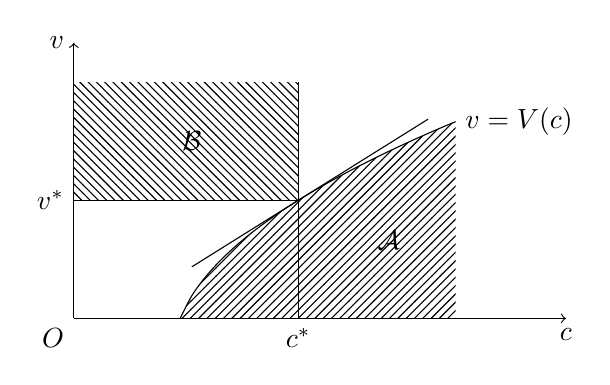
\begin{tikzpicture}[scale=2.5]
    % 绘制坐标轴
    \draw[->] (0,0) -- (2.5,0) node[below] {$c$};
    \draw[->] (0,0) -- (0,1.4) node[left] {$v$};
    \draw[black] (0,0) node[below left] {$O$};
    
\fill[pattern=north east lines, domain=0.54:1.94, smooth, variable=\x] plot ({\x},{sqrt(\x-0.5)-0.2}) -- (1.94,0) -- (0.54,0) -- cycle;
\draw[domain=0.54:1.94, smooth, variable=\x, black] plot ({\x},{sqrt(\x-0.5)-0.2});  % 重新绘制抛物线以覆盖填充边界

\draw[black] (1.14,0) -- (1.14,1.2) ; 
\draw[black] (0,0.6) -- (1.14,0.6) ; 
\draw[black] (0.6,0.2625) -- (1.8,1.0125) ;  

\fill[pattern = north west lines] (0,0.6) -- (1.14,0.6) -- (1.14,1.2) -- (0,1.2) -- cycle;
\filldraw [black] (1.94,1) node[right] {$v=V(c)$}; 
\filldraw [black] (1.14,0) node[below] {$c^*$}; 
\filldraw [black] (0,0.6) node[left] {$v^*$}; 
\filldraw [black] (0.6,0.9) node {$\mathcal{B}$}; 
\filldraw [black] (1.6,0.4) node {$\mathcal{A}$}; 

\end{tikzpicture}
\caption{The value function in concave programming} %最终文档中希望显示的图片标题
\label{Fig7.1} %用于文内引用的标签
\end{figure}

Convex sets are meant to be separated from other convex sets. To do this in the most useful way for the present purpose, choose a point $(c^*, v^*)$ in $\mathcal{A}$ such that $v^* = V(c^*)$. This must be a boundary point, since for any $r > 0$, the point $(c^*,v^* —r)$ is in $\mathcal{A}$ but $(c^*, v^* +r)$ is not. Now define $\mathcal{B}$ as the set of all points $(c,v)$ such that $r \leq c^*$ and $v \geq v^*$, that is, revenue $v$ cannot be attained with inputs $c$ except when $c = c^*$ and $v = v^*$. Thus the set $\mathcal{B}$ serves the same role as the corresponding set in Chapter 6. Clearly $\mathcal{B}$ is a convex set with a non—empty interior, and $\mathcal{A}$ and $\mathcal{B}$ have only boundary points in common. Therefore the Separation Theorem can be applied. For reasons that will become clear in a moment, I write the equation of the separating hyperplane as
\begin{equation*}
\iota v - \lambda c = b = \iota v^* - \lambda c^*
\end{equation*}
where $\iota$ is a scalar, $\lambda$ is an $m$-dimensional row vector, and the signs are so chosen that
\begin{equation} \label{equa7.3}
\iota v - \lambda c \left\{  
\begin{array}{ll}
\leq b \quad \mbox{for all} \  (c,v) \in \mathcal{A} \\
\geq b \quad \mbox{for all} \  (c,v) \in \mathcal{B}
\end{array}
 \right.
\end{equation}

The first point to note is that $\iota$ and $\lambda$ must both be non-negative. For example, suppose $\iota$ is negative. Now consider the point $(c^*, v^*+1)$, which is clearly in $\mathcal{B}$. We have
\begin{equation*}
\iota (v^* +1) - \lambda c^* = b - \iota < b
\end{equation*}
which contradicts the separation property. Similarly, for each $i=1,2,\dots,m$, considering points $(c^* - c^i, v^*)$, where $e^i$ is a vector with its $i$th component equal to 1 and all other components zero, we see that $\lambda_i$ cannot be negative.

Now comes a more subtle question: can $\iota$ equal zero? Let us see the consequences of that. For the equation of the hyperplane to be meaningful, the combined vector $(\iota, \lambda)$ must be non-zero. If $\iota =0$, therefore, at least one component of $\lambda$ must be non-zero, that is, positive. The equation of the separating hyperplane becomes $-\lambda c = -\lambda c^*$, or $\lambda (c-c^*) \geq 0$. In the scalar constraint case, the separating line is vertical at $c^*$, and the set $\mathcal{A}$ lies entirely to the right of it.

Figure 7.2 shows two ways in which this can happen. In both cases, there are no feasible points to the left of $c^*$; production is impossible if input supply falls short of this level. In some applications, this can happen because of indivisibilities. The two cases
differ in the behavior of $V(c)$ as $c$ approaches $c^*$ from the right. In case (a), the marginal revenue product of the resource goes to infinity, and only a vertical separating line will do. In case (b), the limit of the marginal revenue product stays finite, and While a vertical separating line exists, there are also many other separating lines with finite slope, and therefore positive $\iota$. This shows that the conditions soon to be found for ensuring a positive $\iota$ are only sufficient and not necessary.

\begin{figure}[!htp]  % 常见htbp  here top bottom p表示浮动  !表示忽略“美学”标准
 \centering
 \subfloat[ ] %第一张子图
 {
   \begin{minipage}{0.5\linewidth}
\centering
        \begin{tikzpicture}[scale=2]
    % 绘制坐标轴
    \draw[->] (0,0) -- (2.5,0) node[below] {$c$};
    \draw[->] (0,0) -- (0,2.5) node[left] {$v$};
    \draw[black] (0,0) node[below left] {$O$};

\draw[black] (0,1) node[left] {$v^*$};
\draw[black] (1,0) node[below ] {$c^*$};
\filldraw [black] (0.5,1.5) node {$\mathcal{B}$}; 
\filldraw [black] (1.6,0.6) node {$\mathcal{A}$}; 
\filldraw [black] (1.7,1.5) node {$v=V(c)$}; 

    \draw[domain=1:2,smooth,variable=\x] plot ({\x},{ 1+sqrt(1- (\x-2)*(\x-2) )}) ;
    \draw[] (1,0) -- (1,2.2) ; 
    \draw[] (0,1) -- (1,1);
        \end{tikzpicture}
   \end{minipage} }
 \subfloat[ ] %第二张子图
   {
   \begin{minipage}{0.5\linewidth}
\centering
       \begin{tikzpicture}[scale=2]
    % 绘制坐标轴
    \draw[->] (0,0) -- (2.5,0) node[below] {$c$};
    \draw[->] (0,0) -- (0,2.5) node[left] {$v$};
    \draw[black] (0,0) node[below left] {$O$};

\draw[black] (0,1) node[left] {$v^*$};
\draw[black] (1,0) node[below ] {$c^*$};
\filldraw [black] (0.5,1.5) node {$\mathcal{B}$}; 
\filldraw [black] (1.6,0.4) node {$\mathcal{A}$}; 
\filldraw [black] (1.7,1.0) node {$v=V(c)$}; 
    \draw[] (1,0) -- (1,2.2) ; 
    \draw[] (0,1) -- (1,1);
    \draw[] (1,1) -- (2,1.5);
\draw[domain=0.6:1.6,smooth,variable=\x] plot ({\x},{ 2*\x -1  }) ;

      \end{tikzpicture}
   \end{minipage} }
 \caption{Failure of the constraint qualification} 
\label{Fig7.2} 
\end{figure}

The natural condition is to rule out indivisibility. If the set $\mathcal{A}$ has any points to the left of $c^*$, then it cannot have an infinite slope at $c^*$. For this, there must be an $x^o$ such that $G(x^o) < c^*$ and $F(x^o)$ is defined; then we can choose $(G(x^o), F(x^o))$ as the desired point in $\mathcal{A}$. If there are several constraints, we need the corresponding vector inequality $G(x^o) \ll c^*$. This then is the \textit{constraint qualification} for the concave programming problem. It is sometimes called the \textit{Slater condition}.

To prove that the Slater condition implies a positive $\iota$, suppose that the condition holds but $\iota=0$. Then at least one component of $\lambda$ must be positive. Now every component of $G(x^o) - c^*$ is strictly negative. Then
\begin{equation*}
\lambda [G(x^o) - c^*] = \sum\limits_{i=1}^m \lambda_i [G^i(x^o) - c_i^*] < 0
\end{equation*}
because at least one component product on the right-hand side is negative, and all are non-positive. But the point $(G(x^o), F(x^o))$ is in $\mathcal{A}$, therefore by the separation property
\begin{equation*}
- \lambda G(x^o)  =  \iota F(x^o) - \lambda_i G(x^o) \leq \iota v^* - \lambda c^* =  - \lambda c^*
\end{equation*}
or $\lambda [G(x^o) - c^*] \geq 0$. We have proved the same expression to be both negative and non-negative; the contradiction forces us to conclude that the supposition $\iota=0$ must be wrong.

The separation property (\ref{equa7.3}) is unaffected if we multiply $b$, $\iota$, and every component of $\lambda$ by the same positive number. Once we can be sure that $\iota \neq 0$, we can choose this scale to make $\iota = 1$. In economic terms, $\iota$ and $\lambda$ constitute a system of shadow prices, $\iota$ for the revenue and $\lambda$ for the inputs. Only relative prices matter for economic decisions, and in setting $\iota =1$, we are choosing revenue to be the numeraire. This seems an obvious choice, and I shall adopt it henceforth. But sometimes we might wish to do otherwise; for example $F(x)$ might give the revenue in a foreign currency, and then $\iota$ would be an exchange rate to convert it into domestic currency units. The important thing is to establish conditions under which the marginal revenue product of inputs at the optimum is finite, ensuring that the proposed numeraire is not a free good.

Next observe that by the separation property, $c^*, v^*)$ achieves the maximum value of $(v — \lambda c)$ among all points $(c,v) \in \mathcal{A}$. This has an important economic implication. If we interpret $\lambda$ as the vector of shadow prices of the inputs, then $(v — \lambda c)$ is the profit that accrues when a producer uses inputs $c$ to produce revenue $v$. Since all points in $\mathcal{A}$ represent feasible production plans of this kind, the result says that a profit-maximizing producer will pick $(c^*, v^*)$. He need not be aware that in fact the availability of inputs is limited to $c^*$. He may think himself free to choose any $c$, but ends up choosing the right $c^*$. The prices $\lambda$ bring home to him the scarcity. The interpretation is special, but the principle is general and important: constrained choice can be converted into unconstrained choice if the proper scarcity costs or shadow values of the constraints are netted out of the criterion function. To the economist, this is the most important feature of Lagrange's Method in concave programming.

The shadow price interpretation of $\lambda$ can be confirmed some what more formally. For any $c$, the point $(c, V(c))$ is in $\mathcal{A}$. So by the separation property we have
\begin{equation*}
V(c) - \lambda c \leq V(c^*) - \lambda c^*
\end{equation*}
or
\begin{equation} \label{equa7.4}
V(c) - V(c^*) \leq \lambda (c-c^*)
\end{equation}
The linear function on the right overestimates changes in the value of $V$. This looks very much like the concavity property (\ref{equa7.1}), and suggests that $\lambda$ should equal $V_c(c^*)$, the vector of partial derivatives of $V$ at $c^*$. That would make $\lambda$ the vector of the marginal revenue products of the inputs at the optimum, or the vector of shadow prices for the constraints. But one difficulty remains: we cannot be sure that $V$ is differentiable. So far in this chapter we have not even assumed $F$ and $G$ to be differentiable, but even when we do, $V$ may fail to be. This can happen for the same reason as we saw in Chapter 4 and Figure \ref{Fig4.1}. Different inequality constraints may hold as exact equalities for different ranges of the parameters, and where the solution switches from one regime to another, the slope of $V$ may change suddenly.

Even when such discontinuities in the slope of $V$ exist, a very natural generalization of the concept of diminishing returns holds. As the value of some component of $c$ increases, the corresponding partial derivative of $V$ may jump downward, but not upward. This follows from the concavity of $V$.

The asterisks, having served their purpose of distinguishing a particular point in the $(c,v)$ space for separation, may now be dropped. Let us consider a general point $(c, V(c))$ with its associated multiplier vector $\lambda$. Compare this with a neighboring point where only the $i$th input is increased: $(c+he^i, V(c+he^i))$ where $h$ is a positive scalar and $e^i$ is a vector with its $i$th component equal to 1 and all others zero. Then (\ref{equa7.4}) becomes
\begin{equation*}
V(c+he^i) - V(c) \leq \lambda h e^i = h \lambda_i
\end{equation*}
Since $h$ is positive, we can divide by it to write
\begin{equation*}
  [V(c+he^i ) -V(c)] /h \leq \lambda_i
\end{equation*}
It is easy to show that by the concavity of $V$, the left-hand side is a non-increasing function of $h$, and therefore must have a limit as $h$ goes to zero from positive values. In a diagram showing $c_i$ and $V(c)$, the expression on the left-hand side is simply the slope of a chord joining the point $(c, V(c))$ to an adjacent point to the right (because $h>0$). Its limit is defined as the `rightward' partial derivative of $V$ with respect to the $i$th coordinate of $c$, and written $V_i^+(c)$. Thus we have proved that $V_i^+(c) \leq \lambda_i$.

Next repeat the procedure but let $h$ be negative. Now division by $h$ reverses the direction of the inequality, and taking the limit from negative values of $h$ gives us the `leftward' partial derivative $V_i^-(c)$. This proves $V_i^-(c) \geq \lambda_i$. Combining the two, we have the final result that generalizes the notion of diminishing marginal products:
\begin{equation} \label{equa7.5}
V_i^-(c) \geq \lambda_i \geq V_i^+(c)
\end{equation}
Figure \ref{Fig7.3} illustrates this for the case of a scalar $c$.
\begin{figure}[!htb] %H为当前位置,!htb为忽略美学标准,htbp为浮动图形
\centering %图片居中
%\includegraphics[width=0.8\textwidth]{./Fig3.1.png} %插入图片,[]中设置图片大小,{}中是图片文件名
\begin{tikzpicture}[scale=2.5]
    % 绘制坐标轴
    \draw[->] (0,0) -- (2,0) node[below] {$c$};
    \draw[->] (0,0) -- (0,2) node[left] {$v$};
    \draw[black] (0,0) node[below left] {$O$};
    
\draw[black] (1.6,1.6) node[right] {$V_+^\prime(c)$};
\draw[black] (1.4,1.6) node[above] {$\lambda$};
\draw[black] (0.6,0.2) node[left] {$V_-^\prime(c)$};
\draw[domain=1:1.6, smooth, variable=\x, black, line width=1pt] plot ({\x},{1+ln(\x)});  
\draw[domain=0.78:1, smooth, variable=\x, black, line width=1pt] plot ({\x},{2*sqrt(\x -0.75)});  

\draw[] (0.6,0.6) -- (1.6,1.6);
\draw[domain=0.6:1.3, smooth, variable=\x, black] plot ({\x},{2*\x -1});  
\draw[domain=0.6:1.4, smooth, variable=\x, black] plot ({\x},{1.5*\x -0.5}); 
\end{tikzpicture}
\caption{Generalized marginal products} %最终文档中希望显示的图片标题
\label{Fig7.3} %用于文内引用的标签
\end{figure}

So far the vector of choice variables, $x$, has been kept in the background. Let us bring it in explicitly. Recall that $\bar{x}$ maximizes $F(x)$  subject to $G(x ) \leq c$. Let $\lambda$ be the vector of shadow prices of inputs found from the separating hyperplane as in Figure \ref{Fig7.1}. The point $(F(\bar{x}), G(\bar{x}))$ is in $\mathcal{A}$, so the separation property gives
\begin{equation} \label{equa7.6}
F(\bar{x}) -\lambda G(\bar{x}) \leq V(c) - \lambda c
\end{equation}
Of course $F(\bar{x} = V(c))$, so
\begin{equation} \label{equa7.7}
\lambda [c- G(\bar{x})] \leq 0
\end{equation}
Now every component of the row vector $\lambda$ is non-negative, and every component of the column vector $[c- G(\bar{x})]$ is also non-negative. Therefore for every $i$, the product $\lambda_i [c_i - G^i(\bar{x})]$ is non-negative. The inner product in (\ref{equa7.7}) is the sum of these terms. It can be non-positive only if each term is zero. Therefore for every $i$, either $\lambda_i =0$ or $c_i -G^i(\bar{x}) =0$. This is just the notion of complementary slackness developed in Chapter 3, and it fits in well with the interpretation of $\lambda_i$ as the shadow price of the $i$th constraint. The shadow price of any slack constraint is zero, and any constraint with a positive shadow price must be binding. Note an implication of complementary slackness: the inequalities in (\ref{equa7.6}) and (\ref{equa7.7}) must in fact hold as equations.

Finally, since $(F(x), G(x))$ is in $\mathcal{A}$ for any $x$, and since (\ref{equa7.6} ) holds as an equation because of complementary slackness, the separation property gives
\begin{equation} \label{equa7.8}
F(x) - \lambda G(x) \leq F(\bar{x}) - \lambda G(\bar{x})
\end{equation}
for all $x$. That is, $\bar{x}$ maximizes $F(x) -\lambda G(x) $ without any constraints. This is an alternative statement, in terms of underlying choice variables, of how shadow prices allow us to convert the original constrained revenue-maximization problem into an unconstrained profit-maximization problem.

All of the above reasoning can now be summarized into the basic theorem of this section:

\textit{Necessary conditions of Concave Programming:} Suppose that $F$ is a concave function and $G$ is a vector convex function, and that there exists an $x^o$ satisfying $G(x^o) \ll c$. If $\bar{x}$ maximizes $F(x)$ subject to $G(x) \leq c$, then there is a row vector $\lambda$ such that (i) $\bar{x}$ maximizes $F(x) - \lambda G(x)$ without any constraints, and (ii) $\lambda \geq 0$, $G(\bar{x}) \leq c$ with complementary slackness.

None of this requires $F$ and $G$ to have derivatives. But if the functions are differentiable, then we have the first-order necessary conditions for the maximization in (i), namely
\begin{equation} \label{equa7.9}
F_x(\bar{x}) - \lambda G_x(\bar{x}) =0
\end{equation}
In terms of the Lagrangian $L(x,\lambda)$ of Chapter 3, (\ref{equa7.9}) becomes $L_x(\bar{x}, \lambda) =0$. This is just the condition (\ref{equa3.5}) of Lagrange's Theorem with Inequality Constraints. Here I did not impose any non-negativity constraints on the choice variables $x$, but that was just to keep the algebra as simple as possible. Such conditions can be added on without causing any new difficulties, and then we get the corresponding condition (\ref{equa3.7}) of the Kuhn-Tucker Theorem. I leave it as an exercise for the reader to verify this.

There is one respect in which concave programming goes beyond the general Lagrange or Kuhn—Tucker conditions. The conditions of Chapter 3 merely set the first-order derivatives of the Lagrangian with respect to the choice variables equal to zero. This was not sufficient to ensure maximization, and in general there was no claim that $\bar{x}$ is maximized the Lagrangian. When $F$ is concave and $G$ is convex, part (i) of the above theorem on Concave Progamming is easily transformed into $L(x, \lambda) \leq L(\bar{x}, \lambda)$ for all $x$, so $\bar{x}$ does maximize the Lagrangian. The distinction does make economic sense: we know that profit-maximization at given prices can be problematic when there are economies of scale. Price must still equal marginal cost at the optimum, but profit need not be maximized, even in comparison with neighboring points. In the same way, our interpretation of Lagrange‘s method as converting constrained revenue-maximization into unconstrained profit-maximization must be confined to the case of concave programming.

The previous paragraph was on the verge of saying that the first-order conditions are sufficient to yield a true maximum in the concave programming problem. That is indeed so. The argument proceeds in two parts.

First, suppose $\bar{x}$ satisfies the conditions (i) and (ii) in the statement of the necessary conditions. Then, for any $x$, we have
\begin{equation*}
F(\bar{x}) - \lambda G(\bar{x}) \geq F(x) - \lambda G(x)
\end{equation*}
or using complementary slackness, 
\begin{equation*}
F(\bar{x}) - \lambda c \geq F(x) - \lambda G(x)
\end{equation*}
If $x$ is feasible, $G(x) \leq c$, and then
\begin{equation*}
F(\bar{x}) \geq  F(x) + \lambda [c - G(x)]  \geq F(x) 
\end{equation*}

Next suppose $\bar{x}$ satisfies the first-order conditions (\ref{equa7.9}). Since $F$ is concave, $G$ is convex, and $\lambda \geq 0$, $F-\lambda G$ is concave. Then (\ref{equa7.1} ) applied to this function gives
\begin{equation*}
[F(x) - \lambda G(x)] - [F(\bar{x}) - \lambda G(\bar{x})]  \leq [F_x(\bar{x}) - \lambda G_x(\bar{x})](x -\bar{x})
\end{equation*}
But the right hand side is zero by (\ref{equa7.9}). Therefore
\begin{equation*}
 F(x) - \lambda G(x) \leq F(\bar{x}) - \lambda G(\bar{x}) 
\end{equation*}
or $\bar{x}$ maximizes $F(x) -\lambda G(x)$ without any constraints.

This is summed up in the next theorem:

\textit{Sufficient Conditions for Concave Programming:} If $\bar{x}$ and $\lambda$ are such that 
\begin{itemize}
\item[(i)] $\bar{x}$ maximizes $F(x) - \lambda G(x)$ without any constraints, and 
\item[(ii)] $\lambda \geq 0$, $G(\bar{x}) \leq c$ with complementary slackness,
\end{itemize}
then $\bar{x}$ maximizes $F(x)$ subject to $G(x) \leq c$. If $(F-\lambda G)$ is concave (for which in turn it suffices to have $F$ concave and $G$ convex), then (\ref{equa7.9}) implies (i) above.

Note that no constraint qualification appears in the sufficient conditions; it pertains to the validity of the necessary conditions.

\section*{Quasi-Concave Programming}

In the separation approach of Chapter 6, $F$ was merely quasi-concave and each component constraint function in $G$ was quasi-convex. In this chapter the stronger assumption of concavity and convexity has been made so far. In fact the weaker assumptions of quasi-concavity and -convexity make little difference to the necessary conditions. They yield sufficient conditions like the ones above for concave programming, but only in the presence of some further technical conditions that are quite complex to establish. Therefore I shall discuss only a limited version of quasi-concave programming, namely one where the objective function is quasi-concave and the constraint function is linear. Of course the mirror—image case of a linear objective and a quasi-convex constraint can be treated in the same way. Therefore my analysis covers each of the decentralized pair of decision problems into which the separation approach of Chapter 6 split the general quasi—concave programming problem.

First we must establish a property of quasi-concave functions that is similar to the `overestimation by the tangent' property of concave functions. Start with the definition: if $F$ is quasi-concave, then for any $x^a$ and $x^b$ and for any $\theta$ in [0,1], we are to have
\begin{equation*}
F[(1-\theta)x^a + \theta x^b] \geq \min [F(x^a), F(x^b)]
\end{equation*}
Suppose $F(x^b) \geq F(x^a)$. Then
\begin{equation*}
F[ x^a + \theta (x^b - x^a)] \geq F(x^a)
\end{equation*}
Fix $x^a$, $x^b$, and regard the left-hand side as a function of $\theta$, say $h(\theta)$. Then the inequality is simply
\begin{equation*}
 h(\theta) \geq h(0) \quad \mbox{for all } \theta \geq 0 \ \mbox{and} \leq 1
\end{equation*}
Therefore $h^\prime(0) \geq 0$. But by the chain rule,
\begin{equation*}
 h^\prime(\theta) = F_x[x^a + \theta (x^b - x^a)]  (x^b - x^a)
\end{equation*}
Evaluating this at $\theta =0$, we have
\begin{equation} \label{equa7.10}
F_x(x^a) (x^b - x^a) \geq 0
\end{equation}
This holds for all $x^a$, $x^b$ such that $F(x^b) \geq F(x^a)$. Note that $F_x$ is a row vector, so the expression on the left-hand side is an inner product.

Now consider the maximization of $F(x)$ subject to $px \leq b$, where $p$ is a row vector and $b$ a number. The necessary conditions for $\bar{x}$ to be optimum are 
\begin{equation} \label{equa7.11}
F_x(\bar{x}) - \lambda p = 0
\end{equation}
If $\lambda > 0$ the constraint is binding, and this is the only case I shall consider. (By taking cubic transforms of $F$, it is possible to get spurious stationary points where (\ref{equa7.11}) holds with $\lambda =0$, but that is not a case of sufficient economic interest for an elementary exposition.) The aim is to prove that if $F$ is continuous and quasi-concave, the conditions (\ref{equa7.11}) are also sufficient. That is, if they are satisfied by $\bar{x}$ and $\lambda >0$, then $\bar{x}$ solves the quasi-concave programming problem.

To prove this, consider any $x$ such that $F(x) > F(\bar{x}) \equiv \bar{v}$. I shall prove that $x$ is not feasible, that is, $px > b$. Start by using (\ref{equa7.10}) with $x^a = \bar{x}$ and $x^b = \bar{x}$. Then $F(x) > F(\bar{x})$ implies
\begin{equation*}
F_x(\bar{x}) (x-\bar{x}) \geq 0
\end{equation*}
Substitute (\ref{equa7.11}) into this and divide by the positive number $\lambda$ to get
\begin{equation*}
p(x - \bar{x}) \geq 0, \quad \mbox{or} \quad px \geq p \bar{x}
\end{equation*}
In other words, the upper contour set of $F(x)$ for the value $\bar{v}$ is contained in the half of the $x$-space on or above the constraint line.

Figure \ref{Fig7.4} illustrates this. Geometrically, the vector $F_x(\bar{x})$ is normal (perpendicular) to the contour of $F(x)$ at $\bar{x}$. The vector $p$ is normal to the constraint line $px =b $ at any point on it. The usual condition of tangency between the two curves is equivalent to saying that their normal vectors be parallel. That is just what (\ref{equa7.11}) expresses, with the constant of proportionality equal to $\lambda$.
\begin{figure}[!htb] %H为当前位置,!htb为忽略美学标准,htbp为浮动图形
\centering %图片居中
%\includegraphics[width=0.8\textwidth]{./Fig3.1.png} %插入图片,[]中设置图片大小,{}中是图片文件名
\begin{tikzpicture}[scale=2]
    % 绘制坐标轴
    \draw[->] (0,0) -- (3,0) node[below] {$x_1$};
    \draw[->] (0,0) -- (0,3) node[left] {$x_2$};
    \draw[black] (0,0) node[below left] {$O$};
    \draw[black] (1.9,0.7) node[below] {$px= p\bar{x}$};
\draw[black] (2,1) node[right] {$F(x)= F(\bar{x} )$}; 
\draw[domain=1:2, smooth, variable=\x, black] plot ({\x},{2-sqrt(-3+4*\x-\x*\x)});  
\draw[domain=0.7:1.9, smooth, variable=\x, black] plot ({\x},{ -\x +4-sqrt(2)  } );  
 
\filldraw [black]  ({2-1/sqrt(2)}, {2-1/sqrt(2)}) circle (1pt) node [below left] {$\bar{x}$} ;
\draw[->]  ({2-1/sqrt(2)}, {2-1/sqrt(2)}) -- (1.8,1.8) node[above] {$ F_x(\bar{x}) =\lambda p$} ;

\end{tikzpicture}
\caption{Quasi-concave objective and linear constraint} %最终文档中希望显示的图片标题
\label{Fig7.4} %用于文内引用的标签
\end{figure}

Since $F$ is continuous and $F(x) > F(\bar{x})$, in fact $x$ is an interior point of the upper contour set. Therefore it is also an interior point of the set $px \geq b$. In other words, it satisfies $px >b$. So any $x$ yielding value greater than $F(\bar{x})$ is infeasible, or any feasible $x$ yields no greater value than $F(x)$. This completes the proof.

\section*{Uniqueness}

The above sufficient conditions for concave as well as quasi—concave programming are \textit{weak} in the sense that they establish that no other feasible choice $x$ can do better than $\bar{x}$. They do not rule out the existence of other feasible choices that yield $F(x) = F(\bar{x})$. In
other words, they do not establish the uniqueness of the optimum. As in Chapter 6, an additional condition, namely a strengthening of the concept of concavity or quasi-concavity, gives uniqueness.

For example, the definition of strict concavity requires all interior points of the chord joining any two points on the graph of the function to lie strictly below the graph. This rules out any straight line segments where the graph and the chord can coincide. Formally, call $F$ strictly concave if, for distinct $x^a$, $x^b$, and for any $\theta$ in [0,1] except the end—points 0 and 1, we have
\begin{equation} \label{equa7.12}
 F[\theta x^a + (1-\theta)x^b] > \theta F(x^a) + (1-\theta) F(x^b)
\end{equation}
If the objective function $F$ in the concave programming problem is strictly concave, then the maximizer $\bar{x}$ is unique. The proof proceeds by assuming another equally good choice, say $\tilde{x}$, and showing that $\frac{1}{2} (\bar{x} + \tilde{x}) $ can do even better. I shall leave the simple details to the reader.

\section*{Examples}

\subsubsection*{\textit{Example 7.1: Linear Programming}}

An important special case of concave programming is the theory of \textit{linear programming}. Here the objective and constraint functions are linear:
\begin{equation*}
F(x) = ax, \quad G(x) = Bx
\end{equation*}
where $a$ is an $n$-dimensional row vector and $B$ an $m \times n$ matrix. Now
\begin{equation*}
F_x(x) = a, \quad G_x(x) = B
\end{equation*}
Sign constraints $x \geq 0$ are also imposed. When the constraint functions are linear, no constraint qualification is needed; interested readers can see the reason for this from the formal development of the Kuhn-Tucker theory in the Appendix.

All the conditions of concave programming are fulfilled, and the appropriate Kuhn—Tucker conditions (\ref{equa3.7}) and (\ref{equa3.10}) are necessary as well as sufficient. There is a small new notational point. In this problem we will have occasion to consider the Lagrange multipliers as variables. Therefore their particular values corresponding to the optimum of the problem at hand will be indicated by placing bars over the corresponding symbols.

The Lagrangian is 
\begin{equation} \label{equa7.13}
 L(x, \lambda) = ax + \lambda (c - Bx)
\end{equation}
and the optimum $\bar{x}$, $\bar{\lambda}$ satisfy the conditions
\begin{equation} \label{equa7.14}
 a - \bar{\lambda} B \leq 0, \bar{x} \geq 0, \quad \mbox{with complementary slackness}
\end{equation}
\begin{equation} \label{equa7.15}
 c - B \bar{x}  \geq 0, \bar{\lambda} \geq 0, \quad \mbox{with complementary slackness}
\end{equation}

Between them, (\ref{equa7.14}) and (\ref{equa7.15}) contain $2^{m+n}$ combinations of patterns of equations and inequalities. Not all of these are permissible. Generally, if $k$ of the constraints in (\ref{equa7.15}) hold with equality, this puts $k$ restrictions on the $n$-dimensional vector $x$. To determine it, we should have $(n—k)$ more conditions from (\ref{equa7.14}), so exactly this number of the non-negativity constraints should bind. When this is the case, the corresponding count for $\lambda$ is also correct. Each such $(\bar{x}, \bar{\lambda})$ pair is called a `basic solution'. The space of parameters $(a,c, B)$ splits into regions, in each of which one basic solution obtains. At the boundaries where two such regions meet, there are additional non-basic solutions where both inequalities in some of the complementary slackness pairs hold as equations.

The transition from one such region to another causes a sudden change in the Lagrange multipliers, and therefore kinks in the maximum value function of the kind we saw in Figure \ref{Fig4.1}.

Now consider a new linear programming problem: find a row vector $y$ to minimize $yc$ subject to the constraints $y B \geq a$, $y \geq 0$, where the vectors $a, c$, and the matrix $B$, are exactly as before. In our maximization terminology, this can be written as
\begin{equation*}
\max (-yc) \quad \mbox{subject to} \quad -yB \leq -a, \ y \geq 0
\end{equation*}
Except for an interchange of row vectors and column vectors, this is of the same form as the above problem involving $x$. Therefore we can introduce a column vector $\mu$ of multipliers, and define the Lagrangian
\begin{equation} \label{equa7.16}
M(y, \mu) = -yc + (-a +yB)\mu 
\end{equation}
The optimum $\bar{y}$ and $\bar{\mu}$ are defined by the necessary and sufficient Kuhn-Tucker conditions
\begin{equation} \label{equa7.17}
  -c + B\bar{\mu} \leq 0, \  \bar{y} \geq 0, \quad \mbox{with complementary slackness}
\end{equation}
\begin{equation} \label{equa7.18}
  -a + \bar{y} B \geq 0, \  \bar{\mu} \geq 0, \quad \mbox{with complementary slackness}
\end{equation}

Now (\ref{equa7.17}) is exactly the same as (\ref{equa7.15}), and (\ref{equa7.18}) is the same as (\ref{equa7.14}), if we replace $\bar{y}$ by $\bar{\lambda}$, and $\bar{\mu}$ by $\bar{x}$. In other words, the optimum $\bar{x}$ and $\bar{\lambda}$ of the original problem solve the new problem, with their roles interchanged: $\bar{\lambda}$ is the optimal vector of the choice variables in the new problem, and $\bar{x}$ is the corresponding vector of the multipliers.

The new problem is said to be \textit{dual} to the original, which is then called the \textit{primal} problem in the pair. This captures an important economic relationship between prices and quantities in economics. The primal problem has the standard interpretation. Let $x$ be the vector of output quantities, and $a$ that of prices or unit values of the outputs. The matrix $B$ contains unit input coefficients, so $Bx$ is the vector of input requirements for producing $x$. Finally, $c$ is the vector of input supplies.

When the optimum $\bar{x}$ is found, the corresponding $\bar{\lambda}$ is the vector of shadow prices of the inputs. We just saw that among all the vectors $\lambda$ that satisfy the constraints $\lambda B \geq a$ and $\lambda \geq 0$, the $\bar{\lambda}$ yields the minimum value of $\lambda c$. Thus the shadow prices minimize the cost of the inputs $c$. Note that the $j$th component of $\lambda B$ is $\Sigma_i \lambda_i B_{ij}$, which is just the cost of the bundle of inputs needed to produce one unit of good $j$ , calculated using the shadow prices of the inputs. Thus the constraint is that the vector of such input costs is at least as great as the vector of the unit values of outputs. In other words, the shadow prices of inputs ensure that no good can make a strictly positive profit — a standard `competitive' condition in economics.

Complementary slackness in (\ref{equa7.14}) ensures that if the unit cost of production of good $j$ actually exceeds its price, that is, production would entail a loss when calculated at the proper shadow prices of inputs, then the good will be produced in zero quantity. Conversely, if good $j$ is produced in positive quantity, then the unit cost exactly equals the price, that is, the profit is exactly zero.

This can be summarized by observing that complementary slackness in (\ref{equa7.14}) implies
\begin{equation*}
 a \bar{x} = \bar{\lambda} B \bar{x}
\end{equation*}
and that in (\ref{equa7.15}) gives
\begin{equation*}
  \bar{\lambda} c = \bar{\lambda} B \bar{x}
\end{equation*}
Combining the two, we have
\begin{equation} \label{equa7.19}
a \bar{x} = \bar{\lambda} c
\end{equation}
This says that the value of the optimum output equals the cost of the factor supplies evaluated at the shadow prices. The result can be interpreted as the familiar circular flow of income, that is, national product equals national income.

Finally, it is easy to check that if we take the dual problem as our starting-point and go through the mechanical steps of finding \textit{its} dual, we return to the primal. In other words, duality is `reflexive'.

This is in essence the duality theory of linear programming except for one point. We took the optimum $\bar{x}$ as our starting-point, paying no attention to the existence of the solution. This may be problematic, either because the constraints may be mutually inconsistent, or because they may define an unbounded feasible set and the objective function may tend to infinity as we proceed out along this unbounded set. I shall leave the treatment of this issue to more advanced texts.

\subsubsection*{\textit{Example 7.2: Failure of Profit-maximization}}

For a scalar $x$, consider the maximization of $F(x) = e^x$ subject to $G(x) \equiv x \leq 1$. Since $F$ is increasing, the optimum occurs at $x=1$. The Kuhn—Tucker conditions apply, and give $\lambda = e$.

But $x=1$ does not maximize $F(x) — \lambda G(x)$ without constraints. In fact $e^x - ex$ can be made arbitrarily large by increasing $x$ beyond 1. Lagrange's method does not convert the original constrained maximization problem into an unconstrained profit-maximization problem. The difficulty is that $F$ is not concave.

\section*{Exercise}

\subsubsection*{\textit{Exercise 7.1: Minimization}}

Develop the theory of minimization of a convex function along lines parallel to those used in this chapter for maximization of a concave function.

\subsubsection*{\textit{Exercise 7.2: Convexity of Maximum Value Function}}

Let $\theta$ be a vector of parameters, and consider the problem of choosing $x$ to maximize $F(x,\theta)$ subject to $G(x) \leq 0$. Let $V(\theta)$ denote the maximum value as a function of the parameters. Prove that if $F$ is convex as a function of $\theta$ for each fixed $x$, then $V$ is convex.

In Chapter 5 we saw geometrically (Figure \ref{Fig5.2}) that the minimum cost of producing a given quantity of output, regarded as a function of input prices, is concave. Derive that formally as a corollary of the above general result.

\subsubsection*{\textit{Exercise 7.3: More on Linear Programming}}

Show that the optimal solution $\bar{x}$ of the linear—programming problem of Example 7.1, and the corresponding vector of multipliers $\bar{\lambda}$, are such that
\begin{equation*}
L(x, \bar{\lambda}) \leq L(\bar{x}, \bar{\lambda}) \leq L(\bar{x}, \lambda)
\end{equation*}
for all non-negative $x$ and $\lambda$. In other words, $\bar{x}$ maximizes the Lagrangian when $\lambda = \bar{\lambda}$, and $\bar{\lambda}$ minimizes the Lagrangian when $x = \bar{x}$. In other words, the graph of the Lagrangian in $(x, \lambda)$ space is shaped like a saddle. Therefore $(\bar{x}, \bar{\lambda})$ is said to be a \textit{saddle-point} of the Lagrangian.

Let $V(a, c)$ denote the maximum value function of the linear-programming problem. Show that $V$ is convex in $a$ for each fixed $c$, and concave in $c$ for each fixed $a$.





\chapter{Second-Order Conditions}

\section*{Local and Global Maxima}

The previous chapter developed sufficient conditions for optimality, using properties like concavity and quasi-concavity. These were defined globally, that is, over the full domain of definition of the functions. For example, a function is called concave if the tangent at \textit{any} point lies on or above the graph of the function, or if the graph lies on or above the chord joining \textit{any} two points of it. Correspondingly, the conditions are sufficient for a global maximum; the $\bar{x}$ satisfying them does at least as well as \textit{any} other feasible $x$. In a sense the conditions are ideal; if they are met, we have no further worry that some distant point somewhere may do better than the one we are looking at. But in many applications the functions do not have the desired property over their whole domain of definition.

In this chapter the focus is on the curvature of the objective and constraint functions in a small neighborhood of the proposed optimum. The conditions are expressed in terms of the second-order derivatives of the functions at this point. Conditions on such derivatives are sufficient for local optima; if they hold, the proposed point does better than all points in a sufficiently small neighborhood of it.

This is a useful property when global conditions are not met. Moreover, it has a valuable by-product. In Chapter 4 I introduced the term \textit{comparative statics} for the general method of comparisons of solutions in response to small changes in parameters. Thus far we have been concerned only with the comparative statics of the maximum value $v$, and not of the optimum choice variables $x$. Now we focus on the latter. It turns out that the second-order conditions play an instrumental role in determining the comparative static responses of the optimum choice variables. Therefore I shall develop the theory of second-order conditions and their application to comparative statics in parallel. I shall start with simple cases where the maximization is not subject to any constraints, and go on to the more complex theory of constrained maximization.

\section*{Unconstrained Maximization} 

First suppose a scalar variable $x$ is being chosen to maximize $F(x)$. Let $\tilde{x}$ be a candidate for the optimum choice, and expand $F(x)$ in a Taylor series around $\bar{x}$:
\begin{equation} \label{equa8.1}
F(x) = F(\bar{x}) + F^\prime(\bar{x})(x-\bar{x}) + \frac{1}{2} F^{\prime \prime}(\bar{x}) (x-\bar{x})^2 + \dots
\end{equation}
The first-order necessary condition for optimality is $F^\prime(\bar{x})=0$. Using it, we can write (\ref{equa8.1}) as
\begin{equation} \label{equa8.2}
F(x) - F(\bar{x}) =  \frac{1}{2} F^{\prime \prime}(\bar{x}) (x-\bar{x})^2 + \dots
\end{equation}

For $x$ near enough to $\bar{x}$, the quadratic term will dominate the higher-order terms (concealed in the \dots) in the Taylor expansion. Therefore if $F^{\prime \prime}(\bar{x})$ is positive, we will be able to find an $x$ near enough to $x$ for which $F(x)>F(\bar{x})$. In other words, $\bar{x}$ will not yield a maximum of $F(x)$ in a small neighborhood. Of course it could not yield a maximum over the whole range of $F$ either. This argument gives us a \textit{second-order necessary} condition for $\bar{x}$ to yield a maximum, local or global, of $F(x)$, namely
\begin{equation} \label{equa8.3}
F^{\prime \prime}(\bar{x}) \leq 0
\end{equation}

If this derivative is negative, then the quadratic term in (\ref{equa8.2}) will be negative. In a small enough interval around $\bar{x}$, we will have $F(x) < F(\bar{x})$, irrespective of the signs of higher-order terms. Thus, given that (\ref{equa8.1}) holds,
\begin{equation} \label{equa8.4}
F^{\prime \prime} (\bar{x}) < 0
\end{equation}
is a \textit{second-order sufficient} condition for $\bar{x}$ to give a \textit{local} maximum of $F(x)$.

Note two points of difference between (\ref{equa8.3}) and (\ref{equa8.4}). The former is a weak inequality while the latter is the corresponding strict inequality. The former is a necessary condition for local or global maxima, while the latter is a sufficient condition for local maxima only. Similar remarks apply to second-order conditions in more general contexts. Therefore I shall concentrate on the local sufficiency role of second-order conditions, and leave it to the readers to formulate the corresponding necessary ones.

A local maximum satisfying the second-order conditions is called a \textit{regular} maximum. If the maximum is `irregular', that is, $F^{\prime \prime}=0$, we have to look at higher-order derivatives. Then $F^{\prime \prime \prime}(\bar{x})=0$ is a necessary condition, and  $F^{\prime \prime \prime \prime}(\bar{x})<0$ is a sufficient condition. I shall leave aside such complications.

Now suppose the problem involves a parameter $\theta$. The first-order condition is 
\begin{equation} \label{equa8.5}
F_x (\bar{x}, \theta)=0
\end{equation}
This implicitly defines $\bar{x}$ as a function of $\theta$, and we need to know how the optimum choice will respond to changes in $\theta$. Differentiating (\ref{equa8.5}) totally, we have
\begin{equation*}
F_{xx}(\bar{x}, \theta) d\bar{x} + F_{x\theta}(x, \theta)d\theta =0
\end{equation*}
or
\begin{equation} \label{equa8.6}
d\bar{x} / d\theta = - F_{x\theta}(x,\theta)/ F_{xx}(x,\theta)
\end{equation}
At a regular maximum, the denominator on the right hand side is negative. Then the sign of $d\bar{x}/d\theta$ is the same as that of the cross partial derivative $F_{x\theta}$ at the optimum. This shows at once how the second-order condition helps us in assessing the qualitative effects of parameter changes on the optimum choice.

As a simple economic illustration, consider a profit maximizing firm whose demand curve, and hence the revenue curve shifts. Let $R(x, \theta)$ be the revenue as a function of output $x$ and a shift parameter $\theta$. Arrange matters so that $R_\theta$ is always positive: an increase in $\theta$ shifts the demand and the revenue curves upward. A  calculation similar to that above will show that an increase in $\theta$ will increase the profit-maximizing output $\bar{x}$ if $R_{x\theta}$ is positive, that is, if the increase in $\theta$ shifts the \textit{marginal} revenue upward. Now it is perfectly possible that as $\theta$ increases, the average revenue (the demand curve) shifts up but the marginal revenue shifts down; what is needed is a twist that reduces the elasticity of demand. Then a favorable shift of demand will cause output to fall. This is what underlies many fond paradoxes ans trick questions in elementary microeconomics courses.

Let us turn to the case of maximization with a vector of choice variables, but still no constraints. Now the Taylor expansion is
\begin{equation} \label{equa8.7}
F(x) = F(\bar{x}) + F_x(\bar{x})(x-\bar{x}) + \frac{1}{2}(x-\bar{x})^TF_{xx}(\bar{x})(x-\bar{x}) + \dots
\end{equation}

Here $F_{xx}$ is the symmetric square matrix of the second-order partial derivatives $F_{jk} \equiv \partial^2 F/ \partial x_j \partial x_k$, the superscript $T$ denotes the transpose operation to change the column vector into a row vector, and the second-order terms are the quadratic form
\begin{equation} \label{equa8.8}
(x-\bar{x})^T F_{xx} (\bar{x}) (x-\bar{x}) = \sum_{j=1}^n \sum_{k=1}^n F_{jk}(\bar{x}) (x_j - \bar{x}_j) (x_k - \bar{x}_k)
\end{equation}

Before turning to the maximization problem, it is useful to note how (\ref{equa8.7}) gives a new characterization of concavity. If $F$ is concave, it lies on or below its tangent, or its value is less than or equal to that given by the Taylor expansion up to first order. For this to be true when $x$ is sufficiently close to $\bar{x}$ where the second-order terms dominate the difference, we must have
\begin{equation*}
(x-\bar{x})^T F_{xx}(\bar{x}) (x-\bar{x}) \leq 0
\end{equation*}
for all $x$.

A quadratic form $y^T M y$, where $M$ is a symmetric matrix, is called \textit{negative definite} if its value is negative for all $y \neq 0$. This corresponds to the following condition on $M$. Consider a principal minor of order $k$ of $M$, that is, the submatrix formed by the elements common to any $k$ rows and the $k$ columns with the same numbers as the chosen rows. The determinant of such a principal minor should have the sign of $(-1)^k$, negative if $k$ is odd and positive if $k$ is even. Moreover, this should hold for every $k$ from 1 to $n$, the dimension of the matrix. In fact it suffices to check this for the \textit{leading} principal minors, namely those formed by taking the first $k$ rows and columns. The form is called \textit{negative semi-definite} it its value is non-positive for all $y$; the conditions for this are the corresponding weak inequalities on the principal minors. With these definitions, we say that $F$ is concave at $\bar{x}$ if $F_{xx(\bar{x})}$ is the matrix of a negative semi-definite quadratic form.

Now consider the maximization problem. The first-order necessary condition is $F_x(\bar{x})=0$, and then the second-order sufficient condition is that the quadratic form on the right-hand side of (\ref{equa8.7}) is negative for all $x \neq \bar{x}$, that is, negative definite. The corresponding necessary condition is that it be negative semi-definite. The objective function need not be concave in the general sense defined in Chapter 6, but it must be concave at the point $\bar{x}$ in the sense just defined.

All this once again helps in doing comparative statics. Suppose a vector of parameters $\theta$ enters the definition of $F$. The first-order condition if $F_x(\bar{x}, \theta)=0$. Differentiating, we have
\begin{equation*}
F_{xx}(\bar{x}, \theta) d\bar{x} + F_{x\theta}(\bar{x}, \theta) d\theta =0
\end{equation*}
which looks exactly like the corresponding equation for the one-variable case, except that now $d\bar{x}$ and $d\theta$ are vectors, and $F_{xx}$ and $F_{x\theta}$ are matrices. The solution for $d\bar{x}$ is 
\begin{equation} \label{equa8.9}
d\bar{x} =- F_{xx}(\bar{x}, \theta)^{-1} F_{x\theta}(\bar{x}, \theta)d\theta
\end{equation}
The inverse of a negative definite matrix is also negative definite, and the information about the sign of its minors can be combined with the information about $F_{x\theta}$ in specific problems to find the signs of the changes in some choice variables as some parameters change. The results with many variables and parameters are thus not as simple or general as those before. But I shall offer one application in Example 8.4.

\section*{Constrained Optimization}

I shall begin with the simplest case of two choice variables and one equation constraint, and then state how its results extend to more general situations. Consider the maximization of $F(x_1, x_2)$ subject to $G(x_1, x_2) =c$, where both $F$ and $G$ are increasing functions of their arguments. Figure \ref{Fig2.1}, \ref{Fig6.1}, and \ref{Fig6.3} considered various aspects of this. The crucial point is the \textit{relative} curvature of the tow contours through the optimum $x$; the contour of $F$ should be more convex than that of $G$. To express this algebraically, and find the second derivative of this function. Begin with the contour of $F(x_1, x_2)$.

The expression for the first-order derivative was obtained in conjunction with the tangency argument of Figure \ref{Fig2.1}. Equation (\ref{equa2.8}) is 

\begin{equation*}
d x_2 / d x_1 = - F_1 (x_1, x_2) / F_2 (x_1, x_2)
\end{equation*}
Now we must differentiate this again, remembering that $x_2$ on the right-hand side is a function of $x_1$. Therefore
\begin{equation*}
\begin{array}{rl}
 \dfrac{d^2 x_2}{d x_1^2} & = \dfrac{d [-F_1/F_2]}{dx_1} \\
         & = - \dfrac{ F_2 ( F_{11} + F_{12} dx_2/dx_1 ) - F_1(F_{21}+F_{22} dx_2/dx_1)}{F_2^2} \\
         & = - \dfrac{ F_2^2 F_{11} - 2 F_1 F_2 F_{12} + F_1^2 F_{22}}{ F_2^3 }
\end{array}
\end{equation*}
The arguments $(x_1, x_2)$ of all the derivatives of $F$ are suppressed for brevity.

A similar expression can be derived for the second derivative along the constraint curve. The second-order sufficient condition for $\bar{x}$ to be a local optimum is that $d^2 x_2 / d x_1^2$ along the $F$ contour should be greater than that along the $G$ contour. Using the first-order necessary conditions
\begin{equation*}
F_j(\bar{x}) = \lambda G_j (\bar{x}) \quad \mbox{for} \quad j=1,2
\end{equation*}
remembering that we are assuming the $F_j$ and $G_j$ to be positive, and simplifying, the second-order condition becomes
\begin{equation} \label{equa8.10}
G_2^2(F_{11} - \lambda G_{11} ) - 2 G_1 G_2 (F_{12} - \lambda G_{12}) + G_1^2 (F_{22}-\lambda G_{22}) < 0
\end{equation}

This is more neatly expressed in matrix notation: evaluated at $\bar{x}$,
\begin{equation} \label{equa8.11}
\det \left[
\begin{array}{ccc}
F_{11} -\lambda G_{11} &  F_{12}-\lambda G_{12} & -G_1 \\
F_{21} -\lambda G_{21} &  F_{22}-\lambda G_{22} & -G_2 \\
-G_1  & -G_2 & 0
\end{array}
\right] > 0
\end{equation}

The conditions for the general problem with $n$ choice variables and $m<n$ equation constraints are a direct generalization of this. In the matrix notation already established, we form the partitioned matrix
\begin{equation*}  
\left[ 
\begin{array}{cc}
F_{xx} -\lambda G_{xx} &  - G_x^T \\
-G_x  &  0
\end{array}  
\right]
\end{equation*}
of course evaluated at $\bar{x}$. The top left partition is $n \times n$, the bottom right is an $m \times m$ matrix of zeros, and the other two partitions are $m \times n$ and $n \times m$ as appropriate.

Consider its square submatrices formed by the last $k$ rows and the corresponding columns. We can let $k$ range from 1 to $(m+n)$, and the submatrix for $k=m+n$ will be the whole matrix. For low values of $k$, the submatrices will be singular because of the large number of zeros in the bottom right corner. But those for which $k=2m$ or more are not necessarily singular. The second order sufficient conditions for a local maximum then impose restrictions on the signs of their determinants. The signs are required to alternate, the first one (that formed by the last $2m$ rows and the corresponding columns) having the sign of $(-1)^m$.

I shall omit the proof, but shall verify that the earlier result $\ref{equa8.11}$ arises as a special case of this. When $n=2$ and $m=1$, there are only two submatrices to consider. The determinant of the submatrix formed by the last two rows and columns is $-G_2^2$, which is negative. This automatically conforms with the requirement that it should have the sign of $(-1)^1$. The next determinant is that of the whole matrix, and the alternation rule requires it to be positive. That is just what (\ref{equa8.11}) expresses.

Note that the successive submatrices start from the lower right hand corner, not the top left. Thus $(F_{xx} - \lambda G_{xx})$ is not involved. It need not have a determinant of any particular sign, let alone be negative definite. Thus $(F -\lambda G)$ need not be concave, and while the first order necessary conditions say that $x$ gives a stationary point of $(F - \lambda G)$, it need not maximize it. This possibility was mentioned
in Chapter 7 and illustrated in Example 7.2; now we see more clearly why it can arise.

As usual, the second order conditions are closely related to questions of comparative statics. Add an $s$-dimensional vector of parameters $\theta$
 to the functions $F$ and $G$ in the above problem. Then the first order conditions are
\begin{equation*}
F_x (\bar{x}, \theta) - \lambda G_x (x, \theta) =0
\end{equation*}
and the constraints are satisfied, so
\begin{equation*}
  G (\bar{x}, \theta) = c
\end{equation*}
The optimum choice vector $\bar{x}$ as well as the vector of multipliers $\lambda$ can change as $\theta$ changes. Differentiating totally, we have
\begin{equation*}
\begin{array}{l}
 \sum\limits_{k=1}^n (\partial^2 F/ \partial x_j \partial x_k) d \bar{x}_k +
\sum\limits_{r=1}^s (\partial^2 F/ \partial x_j \partial \theta_r) d \theta_r \\ 
 -\sum\limits_{i=1}^m \lambda_i \left[ \sum\limits_{k=1}^n (\partial^2 G^i / \partial x_j \partial x_k) d \bar{x}_k + \sum\limits_{r=1}^s (\partial^2 G^i/ \partial x_j \partial \theta_r) d \theta_r  \right] \\
 - \sum\limits_{i=1}^m d \lambda_i \partial G^i / \partial x_j = 0
\end{array}
\end{equation*}
This formidable expression, and a simpler one obtained by total differentiation of the constraint, can both be stated in a much more compact form in matrix notation:
\begin{equation} \label{equa8.12}
\left[
\begin{array}{cc}
F_{xx} - \lambda G_{xx}  & -G_x^T \\
-G_x   & 0
\end{array}
\right]
\left[
\begin{array}{c}
 d \bar{x}   \\
 d \lambda^T
\end{array}
\right] = -
\left[
\begin{array}{cc}
F_{x \theta} - \lambda G_{x \theta}  \\
-G_\theta   
\end{array}
\right] d \theta
\end{equation}
Of course all the derivatives are evaluated at $(\bar{x}, \theta)$.

It should be no surprise that the partitioned matrix on the right hand side is the same as the one involved in the second order conditions. Once again, those conditions give us some information about the solutions. Their use is best demonstrated in particular contexts, and I shall do so in Example 8.4.

Finally, consider the case of inequality constraints: the choice of $x$ to maximize $F(x)$ subject to $G(x) \leq c$. In Chapter 3 we saw that the space of parameters $\theta$ that enter into the definition of the functions $F$ and $G$ splits into several regions. In each region, a subset of the constraints binds (holds with equality), and the rest are slack. Different regions have different patterns of binding and slack constraints. So long as the initial configuration is in the interior of one of these regions, we can consider small deviations from it, treating the binding constraints exactly as in the above theory of equation constraints, and simply forgetting about the constraints that remain slack throughout the exercise. But if the initial point is on the boundary between two regions with different patterns of binding and slack constraints, then deviations to one side will have to be treated using one set of equations, and those to another side using a different set. Our approach based on a common Taylor expansion will not handle this. In fact there is little systematic that can be said in such cases; each has to be handled \textit{ad hoc}. Luckily, optima are perched on the boundary between two regions only for exceptional configurations of parameters, so we need not worry too much about them.

\section*{Envelope Properties}

In Chapter 5 we established the envelope property of the maximum value function of an optimization problem:
\begin{equation*}
V(\theta) = \max\limits_x \{ F(x,\theta) \ | \  G(x) \leq c \}
\end{equation*}
is the upper envelope of the family of functions $F(x, \theta)$ in each of which $x$ is held fixed. If $x^1$ happens to be optimum for $\theta_1$, then $V(\theta)$ and $F(x^1, \theta)$ are tangential at $\theta_1$. Figure \ref{Fig5.1} illustrates this. A relation between the curvatures of the two functions is also apparent from the figure: $V$ is more convex than each $F$. This second order envelope property is the subject of this section.

Chapter 5 subsequently considered a more general problem, where the vector $x$ was partitioned into subvectors $(y,z)$. The $y$ variables always changed optimally as $\theta$ changed, while $z$ were held fixed in a subproblem interpreted as the short run. We saw that provided the short run and long run maximum value functions were differentiable, they had the same slopes when the variables fixed in the short run happened to be at their long run optimum values. Now a related second order property suggests itself: the fewer variables are held fixed, the more convex should the maximum value function be. That is the form in which I shall establish the result.

Continuing the notation of that chapter, let $Z(\theta)$ be the long run optimum values of the $z$ variables, $V(\theta)$ the long run maximum value function, and $V(z, \theta)$ the short run maximum value function. When $\theta$ changes to $\theta^\prime$, we have
\begin{equation*}
  V[  Z(\theta), \theta^\prime ] \leq V[ Z( \theta^\prime ), \theta^\prime ] = V(\theta^\prime)
\end{equation*}
Expanding the two expressions on the left and the right around $\theta$ in Taylor series, we have
\begin{equation*}
\begin{array}{rl}
  V[  Z(\theta), \theta  ] & + V_\theta[ Z(\theta), \theta ](\theta^\prime - \theta) + \dfrac{1}{2} V_{\theta \theta} [ Z(\theta), \theta ](\theta^\prime - \theta)^2 + \dots \\
& \leq V(\theta) + V_\theta(\theta) (\theta^\prime - \theta) + \dfrac{1}{2} V_{\theta \theta} ( \theta )(\theta^\prime - \theta)^2 + \dots
\end{array}
\end{equation*}
The first order envelope property allows us to cancel the first two terms on the left-hand side with those on the right-hand side. This leaves
\begin{equation*}
\{ V_{\theta \theta} [Z(\theta), \theta] - V_{\theta \theta}(\theta) \}(\theta^\prime -\theta)^2 + \dots \leq 0
\end{equation*}
Taking $\theta^\prime$ sufficiently close to $\theta$, the quadratic term dominates the rest of the expansion (concealed in \dots) on the left-hand side. For the inequality to hold in this situation, we must have
\begin{equation} \label{equa8.13}
V_{\theta \theta} [ Z(\theta), \theta ] \leq V_{\theta \theta} (\theta)
\end{equation}
This proves that the long-run maximum value function is at least as convex as the short-run one at the point where the two are tangent. For suitably `regular' maxima, we have a strict inequality like (\ref{equa8.13}). I shall not pursue this refinement, but will take up an important application of (\ref{equa8.13}) in Example 8.2.

\section*{Examples}

\subsubsection*{\textit{Example 8.1: Consumer Theory}}

In Example 5.2 the consumer's expenditure function $E(p,u)$ was defined as the minimum outlay required to attain the utility level $u$ at prices $p$. The compensated demand function $C(p,u)$ was the vector of quantities that solved this cost-minimization problem. The envelope property implied that 
\begin{equation*}
 C(p,u) = E_p (p,u)
\end{equation*}
the vector of price-derivatives of the expenditure function.

In Example 6.2 we showed that the expenditure function was concave. Now we know the characterization of concavity in terms of second-order derivatives, and can use this to obtain useful properties of compensated demand functions.

Differentiating the above relationship, we have
\begin{equation} \label{equa8.14}
  C_p(p,u) = E_{pp}(p,u)
\end{equation}
Since the matrix of second-order derivatives on the right-hand side is symmetric, we have the symmetry of substitution effects of price changes:
\begin{equation*}
 \partial C^j / \partial p_k = \partial C^k / \partial p_j = E_{jk}
\end{equation*}

Next, since $E$ is concave, the matrix on the right-hand side is negative semi-definite. In particular, its diagonal entries, being $1 \times 1$ minors, must be $\leq 0$. Therefore
\begin{equation} \label{equa8.15}
   \partial C^j / \partial p_k  \leq 0 \quad \mbox{for all} \ j
\end{equation}
In other words, the own substitution effects of price changes are non-positive.

The same result follows even more simply from the very concept of a maximum. Manipulation of the `revealed preference' inequalities showing that the optimum does at least as well as any other feasible choice leads us to the desired result. Suppose $p^a$ and $p^b$ are two price vectors, and $x^a$ and $x^b$ the corresponding compensated demands. Both attain the same utility level $u$. Since $x^a$ gives the smaller expenditure when prices are $p^a$ and $x^b$ does the same for $p^b$, we have
\begin{equation*}
  p^a x^a \leq p^a x^b  \quad \mbox{and} \quad p^b x^b \leq p^b x^a
\end{equation*}
Adding the two inequalities together and simplifying,
\begin{equation} \label{equa8.16}
  (p^b - p^a)(x^b - x^a ) \leq 0
\end{equation}
This is a general version of (\ref{equa8.15}): if $p^b$ and $p^a$ differ only in their $j$th component, the product in (\ref{equa8.16}) reduces to
\begin{equation*}
    (p_j^b - p_j^a)(x_j^b - x_j^a) \leq 0
\end{equation*}
showing that the own substitution effect of any price change is non-positive. This argument is more general in another sense: it requires no assumptions of differentiability, quasi-concavity etc. Therefore you should use `revealed preference' arguments whenever possible.

\subsubsection*{\textit{Example 8.2: The LeChatelier Samuelson Principle}}

Consider the consumer's expenditure minimization problem once again, this time focusing on the second-order envelope properties. Consider a change in any one price, say $p_1$. Compare two situations. In the first, the quantities of all goods are free to change optimally. In the second, the quantity of one good, say $x_2$, must be kept fixed at its initially optimal level. Each problem will have its own expenditure function. The first-order envelope property says that, displayed as functions of $p_1$, the two will be tangential at the initial point. The second-order property says that the expenditure function of the first problem (where there is more freedom of choice) will be more concave (remember this is a minimization problem): its second derivative with respect to $p_1$ will be more negative. But the first derivative in each problem is the compensated demand for $x_1$ in that situation. Therefore
\begin{equation*} % \label{equa8.16}
  \left| \dfrac{\partial x_1}{\partial p_1} \right|_{x_2 \mbox{\ free}} \geq  \left| \dfrac{\partial x_1}{\partial p_1} \right|_{x_2 \mbox{\ fixed}}
\end{equation*}
In other words, fixing the quantity of some other good 2 makes the compensated demand for good 1 less responsive to its own price. Roughly speaking, any imposed rigidity in one sector of the economy causes a reduction in the responsiveness to prices in other sectors. This is true irrespective of whether goods 1 and 2 are substitutes or complements. This is known as the LeChatelier Samuelson Principle.

\subsubsection*{\textit{Example 8.3: Derived Demand}}

The cost function of a producer is defined by analogy with the expenditure function of a consumer. If $y$ is a scalar output produced using a vector $x$ of inputs and a production function $f(x)$, we let $w$ be a row vector of input prices and define
\begin{equation}  \label{equa8.17}
 c(w,y) = \min\limits_x \{ wx \ | \ f(x) \geq y    \}
\end{equation}
The properties of this are found by analogy with those of the expenditure function (see Examples 5.2, 6.2, and 8.1). It is increasing in all its arguments, homogeneous of degree 1 in $w$ for each fixed $y$, and concave in $w$ for each fixed $y$. The cost-minimizing input choice vector $x$ is found by differentiating the cost function with respect to the input prices:
\begin{equation} \label{equa8.18}
   x = C_w(w,y)
\end{equation}

In the production context there is a further point of interest. Output has a natural scale whereas utility does not. Therefore the concept of returns to scale is pertinent for a producer's cost function but not for a consumer's expenditure function. In particular, if the returns to scale are constant, then cost is proportional to output, and the cost function has a multiplicatively separable form
\begin{equation}  \label{equa8.19}
   C(w,y) = y c(w)
\end{equation}
The function $c(w)$ is now the minimum cost of producing one unit of output. In elementary microeconomics this is called the average-equals-marginal cost when the cost curve is horizontal; here we go one step further and recognize that the height of this cost curve depends on the input prices.

Now consider a competitive equilibrium of an industry with such a cost curve and a demand curve $D(p)$. When each firm's average or marginal cost is horizontal at $c(w)$, so is the industry's. Its intersection with the demand curve determines the industry equilibrium. The price equals the average (equals marginal) cost:
\begin{equation*}   
   p = c(w)
\end{equation*}
The output is found from the demand curve:
\begin{equation*}   
   y = D(p)
\end{equation*}
Finally, the input demands are found by using the special form (\ref{equa8.19}) in the general result (\ref{equa8.18}):
\begin{equation*}   
   x = y c_w(w)
\end{equation*}
By successive substitution we obtain the industry's demand for inputs as a function of the input prices, when the output market is in equilibrium:
\begin{equation} \label{equa8.20}   
   x = D[ c(w) ] c_w(w)
\end{equation}
This is called the `derived demand', and the next question is to find its derivatives.

The chain rule gives
\begin{equation*}   
   \partial x_j / \partial w_k = D c_{jk} + D^\prime c_k c_j
\end{equation*}
where I have omitted the arguments of the functions for brevity. This is better written as an elasticity:
\begin{equation} \label{equa8.21}   
   \dfrac{w_k}{x_j} \dfrac{\partial x_j}{\partial w_k} = \theta_k (\sigma_{jk} - \eta)
\end{equation}
where $\eta$ is the elasticity of the industry demand curve 
\begin{equation*}   
   \eta = - p D^\prime(p) / D(p)
\end{equation*}
$\theta_k$ is the share of the $k$th input in average cost:
\begin{equation*}   
   \theta_k = w_k x_k / [y c(w)]
\end{equation*}
and $\sigma_{jk}$ is the elasticity of substitution between inputs $j$ and $k$:
\begin{equation*}   
   \sigma_{jk} = c c_{jk} / (c_j c_k)
\end{equation*}
of which a special case was examined in Exercise 5.2.

To interpret (\ref{equa8.21}), it is useful to split the effect of $w_k$ on $x_j$ into two parts. The first is a substitution effect: as relative prices of factors change, the cost-minimizing factor proportions change. As in consumer theory, the sign of this effect is unambiguous when $j=k$; the concavity of $c$ implies $c_{kk} \leq 0$ and so $\sigma_{kk} \leq 0$. When $j \neq k$, the effect depends on whether inputs $j$ and $k$ are substitutes or complements. The other term gives the output effect. An increasing in $w_k$ raises the whole average equals marginal cost schedule, reducing the equilibrium output along the demand curve and thereby the demand for all factors.

\subsubsection*{\textit{Example 8.4: Use of Second-Order Conditions}}

Consider a firm that buys a vector $x$ of inputs at prices $w$, produces output $y=f(x)$, and sells it for revenue $R(y)$. Its profit expressed as a function of the choice variables $x$ and the input prices (parameters) $w$ is 
\begin{equation*}   
   F(x,w) = R[ f(x) ] - wx
\end{equation*}

We can find the effect of a change in $w$ on the optimum $x$ by using the general formula (\ref{equa8.9}). Now $w$ replaces $\theta$, and
\begin{equation*}   
   F_x = -w, \quad f_{xw} = -I
\end{equation*}
where $I$ is the identity matrix. So
\begin{equation*}   
   d \bar{x} = F_{xx} ( \bar{x}, w )^{-1} d w^T
\end{equation*}
where the transpose is taken because $dw$ is a row vector like $w$. Then
\begin{equation*}   
   dw d \bar{x} = dw F_{xx} ( \bar{x}, w )^{-1} d w^T
\end{equation*}
By the second-order necessary conditions the quadratic form is negative semi-definite, so $dw d\bar{x} \leq 0$. If the maximum is regular, that is, if the second-order sufficient conditions are satisfied, then the quadratic form is negative definite, and we have the somewhat stronger result $dw d\bar{x} < 0$.

Next consider a consumer maximizing utility $U(x)$ subject to the budget constraint $px \leq I$. The first-order condition is 
\begin{equation*}   
   U_x(\bar{x} ) = \lambda p
\end{equation*}
and so long as utility is increasing, the budget constraint holds with equality, 
\begin{equation*}   
  p\bar{x}  = I
\end{equation*}
We want to find the pure substitution effect of a price change. So let prices change by $dp$, and at the same time change income by $dI = dp \bar{x}$ to compensate the consumer, where $\bar{x}$ is the optimum choice at the initial $(p, I)$. Then total differentiation of the first-order condition and the budget equation gives a particular version of the general result (\ref{equa8.12}),
\begin{equation*}
\left[
\begin{array}{cc}
    U_{xx} & -p^T \\ -p & 0   
\end{array}
\right] 
\left[ \begin{array}{c}
 d \bar{x} \\ d \lambda
\end{array}   \right] = 
\left[ \begin{array}{c}
 \lambda d p^T \\ 0
\end{array}   \right]
\end{equation*}
Then 
\begin{equation*}
dp \ d \bar{x}  = \dfrac{1}{\lambda}[ d \bar{x}^T \quad d \lambda ]
\left[
\begin{array}{cc}
    U_{xx} & -p^T \\ -p & 0   
\end{array}
\right] 
\left[ \begin{array}{c}
 d \bar{x} \\ d \lambda
\end{array}   \right] 
\end{equation*}
which is negative when the second-order sufficient conditions for a regular maximum hold. This is another way of fixing the sign of the own substitution effect in consumption.

\section*{Exercises}

\subsubsection*{\textit{Exercise 8.1: Production Theory}}

In Exercise 6.2 we examined a firm's profit function
\begin{equation*}   
  \prod (q,p) = \max\limits_{x,y}  \{ qy -px \ | \ G(x,y) \leq 0 \}
\end{equation*}
where $q$ and $p$ are respectively the vectors of prices of outputs and inputs, $y$ and $x$ the corresponding quantity vectors, and the constraint reflects technological feasibility. There er proved that $\prod$ was a convex function of $(q,p)$.

Now you are asked to show that the optimum choices of $y$ and $x$ are given in terms of the partial derivatives of $\prod$ by
\begin{equation*}   
 y = \prod_q (q,p)   \quad x = -\prod_p(q,p)
\end{equation*}
Hence show that output supply curves are upward-sloping and input demand curves are downward-sloping:
\begin{equation*}   
  \partial y_j / \partial q_j \geq 0  \quad  \partial x_k / \partial p_k \leq 0
\end{equation*}
for all $j, k$.

\subsubsection*{\textit{Exercise 8.2: More on Derived Demand}}

Consider a competitive firm like that of Example 8.3, but without the assumption of constant returns to scale. Suppose its total cost function is $C(w,y)$, so the marginal cost is $C_y(w,y)$. Assume that the marginal cost curve is rising, or $C_{yy} >0$. The firm takes the output price $p$ and the input price vector $w$ as given, and maximizes profit. Find the set of equations that determines its input demand vector $x$. Examine the role of the cross-partial derivative $\partial ^2 C / \partial y \partial w_k$ in determining the sign of $\partial x_j / \partial w_k$. Interpret your result.

\subsubsection*{\textit{Exercise 8.3: Minimization}}

Develop second-order conditions for unconstrained and constrained minimization problems by analogy with the maximization problems of the text. You will need to define \textit{positive} definite and semi-definite quadratic forms, and the signs of the principal minors of their matrices.








\chapter{Uncertainty}

\section*{Expected Utility}

In a formal sense, the theory of optimization under uncertainty does not require any new mathematical theory as such. The choice variables lead to random outcomes with objective or subjective probability distributions. The objective functions are appropriate probability weighted averages (expected values). The choices are also subject to some constraints. The general theory developed in the first eight chapters continues to apply. In fact the special structure of problems of choice under uncertainty leads to specific results that were not available in the general mathematics of constrained optimization.

Let us make these ideas a little more precise. Suppose that after the decision at hand has been taken, the world could evolve in any of a number of different ways. These are called different states of the world, or elementary events. Suppose at first that the states are discrete and finite in number, indexed by $i=1,2,\dots,m$. Write $p_i$ for their probabilities, objective or subjective as may be appropriate for the application being considered. These are non-negative and add to one. The economically relevant outcomes in the alternative situations will typically be the levels of income wealth, or profit accruing to the decision-maker. Denote these by $Y_i$. Most of the time I shall take the $Y_i$ to be scalars, but in general they could be vectors. Then we can write a general objective function
\begin{equation*}
F(Y_1, Y_2,\dots, Y_m; p_1, p_2, \dots, p_m)
\end{equation*}
The choice or control variables $x$ will affect some or all of the $Y_i$ and the $p_i$; the $x$ variables may also be subject to some additional constraints. The maximization problem can then be solved by familiar methods.

Under certain restrictions on the preferences, the objective function can be expressed in a special form, namely the mathematical expectation (probability weighted average) of the values of a utility function $U$ of the outcomes in the different states:
\begin{equation} \label{equa9.1}
 \sum\limits_{i=1}^m p_i U(Y_i)
\end{equation}
The function $U$ is called the von Neumann-Morgenstern utility function (of income, wealth, or profit as the case may be), and the whole expression (\ref{equa9.1}) is called the expected utility.

This formulation is very useful in its simplicity and its ability to capture some economically interesting aspects of behavior such as risk-aversion. Therefore it is used almost universally in applications. All the work I discuss is based on it. Since my focus is on the techniques of optimization, I shall not state or discuss the conditions under which expected utility maximization is valid, but refer the readers to the books by Arrow and Kreps cited at the end of the chapter. Recent research has begun to develop more general yet tractable alternatives; see the survey by Machina cited at the end of the chapter.

In most situations, one would not expect the decision-maker to be indifferent to the risk involved in getting one of a whole range of values of $Y$. Suppose there are just two states, with distinct outcome $Y_1$ and $Y_2$, and positive probabilities $p$ and $(1-p)$ respectively. Compare this with an actuarially equivalent alternative, where the mathematical expectation of $Y$, namely $[pY_1 +(1-p)Y_2]$, is received with certainty. A decision-maker who is risk-averse will prefer the sure sum. That is,
\begin{equation*}
U[ pY_1 +(1-p)Y_2  ] > p U(Y_1) +(1-p)U(Y_2)
\end{equation*} 
This just says that $U$ is (strictly) concave in the range $[Y_1, Y_2]$. More generally, strict concavity implies
\begin{equation} \label{equa9.2}
U(\sum\limits_{i=1}^m  p_i Y_i) > \sum\limits_{i=1}^m p_i U(Y_i)
\end{equation}
when the probabilities are positive and the outcomes distinct. If $U$ is twice differentiable, $U^{\prime \prime} <0 $ corresponds to risk aversion.

Once again, the decision variables $x$ affect some or all of the outcomes and probabilities, setting up the basis for an optimization problem. A couple of quick illustrations will develop the economic intuition for this.

First supposes $Y_1 < Y_2$, so the first state entails some loss, at least relative to the second. A natural response would be to purchase insurance. Suppose an advance premium payment of $x$ gets you $X$ if state 1 occurs. If this insurance industry is perfectly competitive, and each firm can pool a large number of independent risks, then insurance will be actuarially fair. Then $pX=x$, or $X=x/p$. Therefore $Y_1$ changes to $(Y_1 -x + x/p)$, and $Y_2$ to $Y_2 -x$; remember that the premium is paid in advance, that is in both states. The value of the objective function becomes
\begin{equation*}
p U(Y_1 -x + x/p) + (1-p) U(Y_2 -x)
\end{equation*}
The first-order condition for $x$ to be optimum is found using the chain rule:
\begin{equation*}
p U^\prime (Y_1 -x + x/p)(1/p - 1) - (1-p) U^\prime (Y_2 -x) =0
\end{equation*}
or
\begin{equation*}
 U^\prime (Y_1 -x + x/p) =  U^\prime (Y_2 -x)
\end{equation*}
If $U^{\prime \prime} <0$, this is also sufficient, and implies $Y_1 -x +x/p = Y_2 -x$. Thus a risk-averse person will buy actuarially fair insurance to the point where the outcomes in different states are equal. He will insure, or hedge, fully.

Next suppose the probability of the bad outcome 1 can be reduced by incurring an expense $z$ in advance. In specific contexts this might mean using a more reliable but more expensive product or exercising more care in the risky activity when the act of being careful causes disutility. Now we make $p$ a function of $z$; this will be decreasing, and since $p$ is bounded below, it will generally be convex. The objective function can be written as
\begin{equation*}
 \phi (z) \equiv p(z) U(Y_1 -z) + [1-p(z)] U(Y_2 -z)
\end{equation*}
Then 
\begin{equation} \label{equa9.3}
\begin{array}{rl}
\phi^\prime (z) =& -p^\prime(z) [ U(Y_2 -z) -  U(Y_1 -z)  ]  \\
&- \{ p(z)U^\prime (Y_1 -z) + [1-p(z)] U^\prime(Y_2 -z)  \}
\end{array}
\end{equation}
The first term on the right-hand side is the expected marginal benefit, of care or quality, being the product of the marginal reduction in the probability of the bad outcome, and the difference in utilities between the two outcomes. The other terms constitute the marginal cost of care or quality. The optimum $z$ is defined by the first-order condition.

Finally, suppose both insurance and care variables are available. The insurance company cannot tell whether care was exercised, it can only observe the outcome. If acturially fair insurance is available, the objective function is
\begin{equation*}
\phi(x,z) \equiv p(z) U[Y_1 -z -x + x/p(z)] + [1-p(z)] U(Y_2 -z-x)
\end{equation*}
The first-order condition with respect to $x$ implies
\begin{equation*}
 Y_1 -z -x + x/p(z) = Y_2 -z-x
\end{equation*}
by the same reasoning as before. Let the common value of these be $Y_0$. Then, by analogy with (\ref{equa9.3}), we have
\begin{equation*}
\begin{array}{rl}
 \phi_z(x,z) =& -p^\prime(z) \{ U(Y_2-z-x) -U[Y_1-z-x+x/p(z)]  \} \\
              & -\{ p(z)U^\prime [Y_1-z-x+x/p(z)] + [1-p(z)]U^\prime(Y_2-z-x)  \} \\
             =& -U^\prime(Y_0) < 0
\end{array}
\end{equation*}
when $x$ is chosen optimally. In words, the marginal benefit from care vanishes when there is full insurance, while the marginal cost stays positive. Therefore the optimum of care occurs at the corner $z=0$. In other words, the availability of full insurance destroys the incentive to exercise costly care. This is known as `moral hazard' in the insurance jargon. In practice, only partial insurance will be available when moral hazard is present.

This is an example of the general problem of asymmetric information: one side in an economic transaction has knowledge of some relevant variable like risk, effort, or quality that the other side lacks. Then the transaction cannot take place in a classical competitive market at arm's length; a contract or an incentive scheme has to be designed to get around the information asymmetry as far as possible. A vast new area of economic theory of such situations has opened up in the last decade or so. I discuss two simple problems of this kind in Example 9.1 and 2, and offer some references for further reading at the end of the chapter.

The rest of this chapter deals with more conventional situations of choice under uncertainty, particularly portfolio choice. This is somewhat more conveniently treated in terms of continuous random variables rather than a finite number of states of the world. Thus we replace the index $i$ by a random variable $r$ defined over the range $[\underline{r}, \overline{r}]$, the probabilities $p_i$ by a density function $f(r)$, and the expected utility expression (\ref{equa9.1}) by 
\begin{equation} \label{equa9.4}
  E[U(Y)]  = \int_{\underline{r}}^{\overline{r}} U[Y(r)] f(r) dr
\end{equation}
The choice variable $x$ will then become an additional argument in the function $Y$ and $f$. The interpretation of risk-aversion parallels (\ref{equa9.2}). The mathematical expectation of $Y$ is 
\begin{equation*}
E(Y) = \int_{\underline{r}}^{\overline{r}} Y(r) f(r) dr
\end{equation*}
Then $U^{\prime \prime}  < 0$ implies
\begin{equation} \label{equa9.5}
 U[E(Y)] > E[U(Y)]
\end{equation}
this is an application of Jensen's Inequality.

\section*{One Safe and One Risky Asset}

An investor has initial wealth $W_0$. Investing $x$ in the risky asset yields the total (principal plus interest) of $x(1+r)$, where $r$ is a random variable with the density function $f(r)$. The safe asset pays zero interest; this can be generalized but it makes the notation a little messier. Now the final (random) wealth is 
\begin{equation} \label{equa9.6}
 W= (W_0 -x) + x(1+r) = W_0 + xr
\end{equation}
The amount $x$ must be in the range $[0, W_0]$; `short sales', and borrowing at the riskless rate to invest in the risky asset, are not allowed. The investor has a strictly concave von Neumann Morgenstern utility function $U$, and choose $x$ to maximize 
\begin{equation} \label{equa9.7}
E[U(W)] = \int_{\underline{r}}^{\overline{r}} U(W_0 +xr) f(r) dr
\end{equation}

Let $\phi(x)$ denote this expression regarded as a function of $x$. Then
\begin{equation*}
\phi^\prime(x) = \int_{\underline{r}}^{\underline{r}} r U^\prime (W_0+xr) f(r) dr=0
\end{equation*}
In particular,
\begin{equation*}
\phi^\prime(0) = U^\prime(W_0) \int_{\underline{r}}^{\underline{r}} r f(r) dr = U^\prime (W_0) E(r)
\end{equation*}
Note that $U^\prime(W_0)$ is non-random, and therefore can be taken outside the integration (summation). If the mathematical expectation (probabilistic average) of the rate of interest on the risky asset is positive, then $\phi^\prime(0)$ is positive, and the optimum $x$ cannot be zero. In other words, the risk-averse investor will buy at least some of an actuarially good investment.

If $\underline{r} >0$, then $\phi^\prime(x)>0$ for all $x$, and it is optimal to put all of $W_0$ in the risky asset. More typically, the investor will hold some of each asset. The first-order condition with respect to $x$ is
\begin{equation} \label{equa9.8}
\int_{\underline{r}}^{\overline{r}} r U^\prime (W_0+xr) f(r)dr =0
\end{equation}
If there is an $x<W_0$ satisfying this, then the concavity of $U$ guarantees that it is the global optimum.

The next obvious step is to study the comparative statics of this choice. First suppose $W_0$ changes. Recognize $W_0$ as a parameter in $\phi$. So the maximand is $\phi(x,W_0)$. Write its partial derivative with respect to $x$ as $\phi_x$, and that with respect to $W_0$ as $\phi_w$. Then the first-order condition is $\phi_x(x, W_0)=0$. Differentiating this totally as in Chapter 8, we find
\begin{equation*}
dx / dW_0 = - \phi_{xw}(x, W_0) / \phi_{xx}(x, W_0)
\end{equation*}
The denominator is negative by the second-order condition, so the sign of the comparative static derivative is the same as the sign of the numerator. Now
\begin{equation} \label{equa9.9}
\phi_{xw}(x,W_0) = \int_{\underline{r}}^{\overline{r}} r U^{\prime \prime}(W_0 +xr) f(r) dr
\end{equation}
Since an interior $x$ can be optimal only if $\underline{r} <0<\overline{r}$, we cannot fix the sign of (\ref{equa9.9}) without further work. The answer turns out to depend on the property of a measure of risk-aversion. Remember that $U^{\prime \prime}<0$ means risk-aversion; a useful quantitative measure of this turns out to be 
\begin{equation} \label{equa9.10}
A(W) = - U^{\prime \prime}(W) / U^\prime(W)
\end{equation}
To interpret this, we consider decreasing the variance of the distribution of $W$ slightly, and asking what decrease in its mean will leave the investor indifferent. This marginal rate of substitution turns out to be $\dfrac{1}{2} A(W)$. A higher $A(W)$ means the investor is willing to give up more of the mean return to get a given small decrease in variance. Therefore $A(W)$ is called the investor's \textit{absolute risk-aversion}. We would expect a wealthier investor to be more tolerant of a given marginal risk, that is $A(W)$ should be a decreasing function.

Then the result is that if the absolute risk-aversion $A(W)$ is a decreasing function of wealth, then $\phi_{xw}$ is positive; that is, a wealthier investor will hold more of the risky asset.

To prove this, note that for $r<0$, we have
\begin{equation*}
 - U^{\prime \prime} (W_0 +xr) / U^\prime (W_0 +xr) > - U^{\prime\prime} (W_0) / U^\prime(W_0) = A(W_0)
\end{equation*}
Multiplying by $-r$,
\begin{equation*}
 r U^{\prime \prime} (W_0 +xr) / U^\prime (W_0 +xr) > -r A(W_0)
\end{equation*}
or 
\begin{equation} \label{equa9.11}
r U^{\prime \prime} (W_0 +xr) > - A(W_0) r  U^\prime (W_0 +xr)
\end{equation}
For $r>0$,
\begin{equation*}
 - U^{\prime \prime} (W_0 +xr) / U^\prime (W_0 +xr) < - U^{\prime\prime} (W_0) / U^\prime(W_0) = A(W_0)
\end{equation*}
Multiplying by $r$,
\begin{equation*}
 -r U^{\prime \prime} (W_0 +xr) / U^\prime (W_0 +xr) < r A(W_0)
\end{equation*}
or 
\begin{equation*}
 r U^{\prime \prime} (W_0 +xr) >  -A(W_0) r U^\prime (W_0 +xr) 
\end{equation*}
once again.

We have shown that the inequality (\ref{equa9.11}) holds for all $r$, positive or negative. Integrating it,
\begin{equation*}
 \int_{\underline{r}}^{\overline{r}} r U^{\prime \prime} (W_0 +xr) f(r)dr > -A(W_0) \int_{\underline{r}}^{\overline{r}} r U^\prime (W_0 +xr) f(r) dr
\end{equation*}
The right-hand side is zero by (\ref{equa9.8}). This proves the result.

The next natural questions are the effects on $x$ of shifts in the density function $f$, particularly an increase in risk, and in the utility function $U$, particularly an increase in risk-aversion. But these topics would take far too much space, and I must leave them to proper microeconomics texts and research articles cited at the end of the chapter.

\section*{Portfolio Choice}

Here we allow any number of risky assets. The treatment of this in financial economics usually assumes that the investor's objective can be expressed as a function of the mean $M$ and the standard deviation $S$ of wealth. This is quite a restrictive assumption. In the expected utility framework, it corresponds to one of two special cases: (1) If the von Neumann-Morgenstern utility function is quadratic,
\begin{equation*}
U(W) = W - \dfrac{1}{2} a W^2
\end{equation*}
where $a>0$ is constant, then
\begin{equation*}
E[U(W)] = M -\dfrac{1}{2} a (M^2 + S^2)
\end{equation*}
(2) If each asset has a normally distributed return, then wealth has a normal distribution, and the expectation of any von Neumann-Morgenstern utility function can be expressed in terms of its mean and variance. A specific function of interest in this context is 
\begin{equation*}
U(W) = -exp(-aW)
\end{equation*}
with $a>0$, for which
\begin{equation*}
E[U(W)] =  - exp(-a[M -\dfrac{1}{2} a S^2]) 
\end{equation*}
Then expected utility is maximized when $(M-\dfrac{1}{2} a S^2)$ is. Using (\ref{equa9.10}), we can see that for this function the absolute risk-aversion is constant and equal to $a$.

In either of the two cases where mean-variance analysis is applicable, the indifference curves of expected utility can be shown in $(M,S)$ space. By constructing the feasible frontier between $M$ and $S$, we can study the portfolio-choice problem diagramatically.

The initial wealth will be held fixed throughout this exercise so normalize it to unity. Suppose there are $n$ assets. Write them total returns (principal plus interest) as a vector $r=(r_1, r_2, \dots, r_n)$. These are random variables. Let their mathematical expectation form a vector $\mu = (\mu_1, \mu_2, \dots, \mu_n)$, and let the (symmetric, positive definite) variance-covariance matrix of the gross returns be $\sum ( \sigma_{ij} )$. The portfolio is a vector of proportions of wealth invested in the various assets, $x=(x_1, x_2, \dots, x_n)$.

The random final wealth is 
\begin{equation*}
W = \sum\limits_{i=1}^n x_i r_i = x^T r
\end{equation*}
The mean and the variance of final wealth are respectively
\begin{equation*}
M = \sum\limits_{i=1}^n x_i \mu_i = x^T \mu
\end{equation*}
and
\begin{equation*}
S^2 = \sum\limits_{i=1}^n \sum\limits_{j=1}^n  x_i x_j \sigma_{ij} = x^T \Sigma x
\end{equation*}
Note that both $M$ and $S^2$ are functions of $x$.

To find the feasible transformation frontier between $M$ and $S$, we want to minimize the standard deviation for a given mean, that is 
\begin{equation*}
\mbox{minimize} \quad S = ( x^T \Sigma x)^1/2, \quad \mbox{subject to} \quad x^T \mu =M, x^T e =1 
\end{equation*}
where $e$ is a vector of ones.

The minimized $S$ is a convex function of $M$. It may have a decreasing portion, but for large $M$ it is increasing, thus presenting a trade-off between return and risk. The case of two assets suffices to bring out the main points, therefore I restrict attention to it here. But the general case illustrates the use of some techniques of optimization from previous chapters; I shall outline it in Example 9.3.

With two assets, let $x$ stand for $x_1$, so $x_2=1-x$. Then
\begin{equation} \label{equa9.12}
M = \mu_2 + (\mu_1 - \mu_2)x
\end{equation}
and 
\begin{equation} \label{equa9.13}
S^2 = \sigma_2^2 -2 K_2 x + (K_1 + K_2) x^2
\end{equation}
where I have defined
\begin{equation*}  
K_1 \equiv \sigma_1^2 - \rho \sigma_1 \sigma_2, \quad K_2 \equiv \sigma_2^2 - \rho \sigma_1 \sigma_2
\end{equation*}
and $\rho$ is the correlation coefficient between the random returns $r_1$ and $r_2$, that is, the covariance divided by the product of their standard deviations.

Order the assets so that $\mu_1 > \mu_2$. Then the equations (\ref{equa9.12}) and (\ref{equa9.13}) define the frontier in $(M,S)$ space in terms of a parameter $x$. As $x$ increases from 0 to 1, $M$ increases from $\mu_2$ to $\mu_1$, and $S$ changes from $\sigma_2$ to $\sigma_1$. Along the way,
\begin{equation} \label{equa9.14}
 S dS /dx = -K_2 + (K_1 + K_2) x
\end{equation}
So
\begin{equation*} 
\mbox{at} \ x=0,  \quad  dS / dx = - (\sigma_2 - \rho \sigma_1)
\end{equation*}
and 
\begin{equation*} 
\mbox{at} \ x=1,  \quad  dS / dx = \sigma_1 - \rho \sigma_2
\end{equation*}

If $\sigma_1 > \sigma_2$, so there is a risk-return trade-off between the two completely specialized portfolios, then $dS/dx$ is sure to be positive near $x=1$, that is, there is bound to be a trade-off over some range of high returns. Even if $\sigma_1 < \sigma_2$, that is, asset 1 dominates asset 2, there may be a diversification benefit from mixing them, and therefore a trade-off, if $\rho$ is sufficiently less than one.

More generally, the minimum-variance portfolio is given by 
\begin{equation*} 
x = \dfrac{K_2}{K_1 + K_2} = \dfrac{\sigma_2^2 - \rho \sigma_1 \sigma_2}{(\sigma_1^2 - \rho \sigma_1 \sigma_2) +(\sigma_2^2 - \rho \sigma_1 \sigma_2)}
\end{equation*} 
The conditions for this to lie in [0,1], that is, not involve any short sales, are evident from the equation.

Differentiating (\ref{equa9.14}) again,
\begin{equation*} 
S d^2 S /dx^2 + (dS / dx)^2 = C
\end{equation*}
Simplifying, we find 
\begin{equation*} 
\mbox{sgn} \ d^2 S / dx^2 = \mbox{sgn} \ (1- \rho^2) \sigma_1^2 \sigma_2^2 >0
\end{equation*}
Therefore the frontier in $(M,S)$ space is convex.

Figure \ref{Fig9.1} sums up the results so far. Two extreme cases are worth pointing out. If $\rho=1$, the frontier is simply the straight line joining $(\mu_1, \sigma_1)$ to $(\mu_2, \sigma_2)$. If $\rho=-1$, then the minimum variance is zero, and the frontier consists of two straight lines joining this riskless portfolio point to each of $(\mu_1, \sigma_1)$ and $(\mu_2, \sigma_2)$.

\begin{figure}[!htb] %H为当前位置,!htb为忽略美学标准,htbp为浮动图形
\centering %图片居中
%\includegraphics[width=0.8\textwidth]{./Fig3.1.png} %插入图片,[]中设置图片大小,{}中是图片文件名
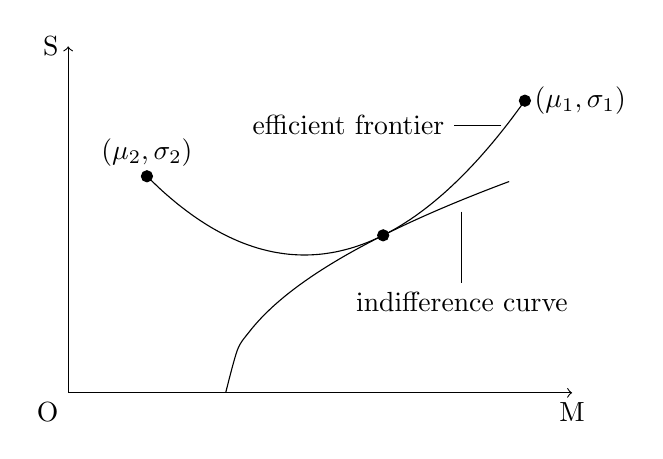
\begin{tikzpicture}[scale=2]
    % 绘制坐标轴
    \draw[->] (0,0) -- (3.2,0) node[below] {M};
    \draw[->] (0,0) -- (0,2.2) node[left] {S};
    \draw[black] (0,0) node[below left] {O};

\draw[domain=1:2.8,smooth,variable=\x, black] plot ({\x},{sqrt(\x-1)}) ;
\draw[domain=0.5:2.9,smooth,variable=\x, black] plot ({\x},{0.5* \x * \x -1.5* \x +2 }) ;

\filldraw [black] (2,1) circle (1pt)   ;
\filldraw [black] (0.5,1.375) circle (1pt)   ;
\draw[black] (0.5,1.375) node[above] {($\mu_2, \sigma_2$)};

\filldraw [black] (2.9,1.855) circle (1pt)   ;
\draw[black] (2.9,1.855) node[right] {($\mu_1, \sigma_1$)};

\draw[black] (2.5,1.15) -- (2.5,0.7) node[below ] {indifference curve};
\draw[black] (2.75,1.7) -- (2.45,1.7) node[left ] {efficient frontier};

\end{tikzpicture}
\caption{Portfolio choice in mean-variance framework} %最终文档中希望显示的图片标题
\label{Fig9.1} %用于文内引用的标签
\end{figure}

Next suppose there is one riskless asset with a sure gross return $\mu_0$, and risky assets are as before. If a fraction $x_0$ of wealth is held in the riskless asset, then
\begin{equation*} 
M = x_0 \mu_0 + x^T \mu = x_0 \mu_0 + (1-x_0) \xi^T  \mu
\end{equation*}
where the vector $\xi$ gives the proportions of the various assets in the risky part of the portfolio. Likewise,
\begin{equation*} 
S^2 = x^T \Sigma x = (1-x_0)^2 \xi^T \Sigma \xi
\end{equation*}
or
\begin{equation*} 
 S=(1-x_0) (\xi^T \Sigma \xi)^{1/2}
\end{equation*}
Therefore the feasible points are found by joining $(\mu_0, 0)$ to each of the points on the frontier previously obtained. In Figure \ref{Fig9.2}, this produces the efficient frontier $ABP_1$ if short sales are not allowed, and the straight-line frontier $ABC$ if they are. In this case the risky assets are only ever held in the proportions represented by the point $B$. Everyone holds a mix of the sure asset and the portfolio $B$, the proportions of this mix depending on the attitude to risk. Thus $B$ becomes a mutual fund.

\begin{figure}[!htb] %H为当前位置,!htb为忽略美学标准,htbp为浮动图形
\centering %图片居中
%\includegraphics[width=0.8\textwidth]{./Fig3.1.png} %插入图片,[]中设置图片大小,{}中是图片文件名
\begin{tikzpicture}[scale=2]
    % 绘制坐标轴
    \draw[->] (0,0) -- (3.2,0) node[below] {M};
    \draw[->] (0,0) -- (0,2.2) node[left] {S};
    \draw[black] (0,0) node[below left] {O};

\draw[domain=0.5:2.9,smooth,variable=\x, black] plot ({\x},{0.5* \x * \x -1.5* \x +2 }) ;

\filldraw [black] (2.2,1.12) circle (1pt) node [below right] {B} ;
 
\draw[black] (0.5,1.375) node[above] {$P_2$};
 
\draw[black] (2.9,1.855) node[above] {$P_1 $};
\draw[-] (0.6,0) -- (3,1.68) node[right] {C};
\draw[black] (0.6,0) node[below ] {A};
\end{tikzpicture}
\caption{Portfolio choice with a riskless asset} %最终文档中希望显示的图片标题
\label{Fig9.2} %用于文内引用的标签
\end{figure}

\section*{Examples}

\subsubsection*{\textit{Example 9.1: Managerial Incentives}}

Eliciting the right amount of effort from subordinates is a problem for capitalist owners and socialist planners alike. Here is a simple example. An owner has to hire a manager to run a project. If the project succeeds, it will produce value $V$. The probability of success depends on the quality of the manager's work. Given high quality, the project will succeed with probability $p$, but low quality will reduce this to $q$. The basic salary needed to attract a manager is $w$. But he has to exert himself  more to achieve high quality, and will do so only if he is paid a premium $e$. Both the owner and the manager are risk-neutral, that is, each maximizes the mathematical expectation of his monetary returns (minus the money-equivalent cost of effort in the case of the manager).

First suppose the owner can observe the quality of the manager's work, and compensate the effort directly. His expected profit from eliciting high-quality work is $pV - (w+e)$, while low-quality operation would get him $qV-w$. The interesting case to consider is one where (a) high quality yields more profit than low quality, that is
\begin{equation} \label{equa9.15}
pV - (w+e) > qV -w \quad \mbox{or} \quad (p-q)V >c
\end{equation}
and (b) the profit with high quality is positive, that is,
\begin{equation} \label{equa9.16}
pV >w+c
\end{equation}

Now suppose the owner cannot observe the quality of effort. If the owner offers the premium $e$ to a manager in return for an unverifiable promise to provide high-quality work, the manager can cheat and deliver low quality instead. This lowers the probability of success of the project, but so long as $1>p>q>0  $, the owner cannot infer the quality of the manager's effort by observing a single success or failure, and therefore has no recourse against the manager's breach of contract.

Therefore the owner must base his payment scheme on the only thing he can observe, namely success or failure. Suppose he pays the manager $x$ if the project succeeds, and $y$ if it fails. Given this scheme, the manager will choose high-quality effort if this gives him greater benefit net of the cost of his effort, that is, if 
\begin{equation*}
px + (1-p)y -e > qx + (1-q)y 
\end{equation*}
If the two sides are equal, the manager is indifferent between high and low-quality effort. It is usual to suppose that so long as it makes no difference to him, he acts like a nice guy and breaks the tie favorably to the owner, that is, chooses high quality. Therefore the inequality is weak rather than strict. It simplifies to 
\begin{equation} \label{equa9.17}
(p-q) (x-y) \geq e
\end{equation}
Secondly, the manager will agree to work for the owner if 
\begin{equation*}
px + (1-p)y \geq w + e
\end{equation*}
or 
\begin{equation} \label{equa9.18}
 y + p(x-y) \geq w+e
\end{equation}
These then are the constraints that give the manager the right incentives.

The owner's expected profit is 
\begin{equation} \label{equa9.19}
\pi = pV - [  px + (1-p)y  ] = pV -y -p(x-y)
\end{equation}
He wants to maximize this subject to the two incentive constraints above. It is obvious that he should make $y$ and $(x-y)$ as small as possible. Then the constraints will hold with equality, and 
\begin{equation*} 
 x-y = e/(p-q) \quad y =w+e - ep/(p-q)
\end{equation*}
or
\begin{equation} \label{equa9.20}
 y = w -e q/(p-q) \quad  x = w +e (1-q)/(p-q)
\end{equation}
These have a simple interpretation: the manager's compensation consists of the basic salary plus a reward for success or minus a penalty for failure.

With these values, the owner's expected profit is
\begin{equation*} 
\pi = pV - w-e
\end{equation*}
the same as when he could observe the manager's effort directly; the inability to observe effort has made no difference.

But there is a difficulty. Nothing guarantees $y \geq 0$. Thus the optimum scheme may involve a fine that the manager pays to the owner if the project fails. In practice such a fine is very difficult to extract. If fines are ruled out, the problem must be solved with an additional constraint $y \geq 0$. The solution is to go as far as possible, namely set $y=0$. Then $x$ must satisfy the remaining two constraints, so 
\begin{equation*}
x \geq (w+e)/p \quad \mbox{and} \quad x \geq e/(p-q)
\end{equation*}
But when the $y$ in the unconstrained solution is negative, $w+e$ is less than $ep/(p-q)$, and the latter is the binding constraint. So $x=e/(p-q)$, and the owner's expected profit is 
\begin{equation*} 
\pi = pV - ep/(p-q)
\end{equation*}
By the conditions (\ref{equa9.15}-\ref{equa9.16}) assumed at the outset, this is less than $pV - w-e$, but still positive. Thus the need to pay output-based incentives means a smaller expected profit, but not by so much as to make the whole enterprise unprofitable.

This example is just the beginning of a large body of recent research on the design of incentive contracts. The problem considered here is similar to that of moral hazard in insurance, where the company could not observe the risk-reducing care on the part of the policyholder. We designed the best contract for a single project. In an ongoing relationship of this kind, the average of the manager's successes over time provides statistical information about his effort, enabling a better contract that generates higher expected profit. Similarly, if the planner has several similar managers who face some common risk, then observation of their relative performance can provide information about their relative efforts. Finally, in the example there was a liquidity constraint - the manager could not be fined - but no risk-aversion. Allowing the manager to be risk-averse brings additional issues of the efficient allocation of risk between the planner and the manager. Some references to the burgeoning literature on such matters are provided at the end of the chapter.

The next example concerns a different problem of information. The planner may not know the innate quality of the manager. This, too, has a parallel in insurance, where the policyholder has better information about his own risk-class than does the company. This gives rise to `adverse selection'; an insurance policy is especially attractive to those who know their own risk to be higher than the odds implicit in the terms of the policy, and who are therefore undesirable customers from the point of view of the company. It wants to design a contract that will handle this problem. For variety, I shall construct the example in a different context.

\subsubsection*{\textit{Example 9.2: Cost-Plus Contracts}}

Government expenditures for defense, health, and yes, even education are often made on a cost-plus basis. That is, the government reimburses the supplier's cost plus a normal profit. The government's purchasing agency usually does not know the true cost of production of these goods or services. If a supplier who can produce the good at low cost pretends to have a higher cost, he gets a higher reimbursement, which he can enjoy by paying high salaries to himself and other workers, spending lavishly on offices and such facilities etc. If the government wishes to avoid the excessive payment, it must devise a scheme that eliminates the temptation to misstate cost. Here is a very simple example.

Suppose the true average cost of production can take just one of two values, $c_1$ and $c_2$, with $c_1 < c_2$. Each figure already includes normal profit. The problem is that the higher figure may be real or pretense; the government cannot tell the difference. In other words, the supplier can be either of two types, low cost or high cost, and the purchasing agency cannot tell whether if faces a genuinely high-cost supplier, or a type-$c_1$ who is pretending to be a type-$c_2$ and planning to enjoy the extra payment.

The government can decide how many units it will buy, and how much it will pay, depending on the cost declared by the supplier. Suppose it announces that if the supplier claims to have the average cost $c_i$, for $i=1$ or 2, it will buy $q_i$ units, and pay a total sum of $R_i$ for them.

What are the constraints on these choices? First, for each of the two cost figures, if that happens to be genuine, the supplier should be willing to participate. That is, his cost should be covered:
\begin{equation} \label{equa9.21}
R_i \geq c_i q_i \quad \mbox{for} \ i=1,2
\end{equation}
Secondly, it should be optimal for the supplier to reveal his true cost. These are called incentive compatibility constraints. If the supplier's true average cost is $c_1$, he should not wish to pretend it is $c_2$, and the other way round. Economic intuition suggests that only the first of these will be binding (a truly high-cost firm will not pretend to be low-cost), but a proper theoretical treatment should prove that, and not assume it at the outset. Now if a firm with cost $c_1$ pretends to have cost $c_2$, it sells $q_2$ units instead of $q_1$, and has revenue $R_2$ instead of $R_1$, but its actual cost in its profit calculation stays at $c_1$. Therefore the constraint for a firm with cost $c_1$ to report it truthfully is 
\begin{equation}\label{equa9.22}
R_1 - c_1 q_1 \geq R_2 - c_1 q_2
\end{equation}
Similarly for a firm with true cost $c_2$, the constraint is 
\begin{equation} \label{equa9.23}
R_2 - c_2 q_2 \geq R_1 - c_2 q_1
\end{equation}

Suppose the government gets benefit $B(q)$ from quantity $q$, where $B$ is an increasing and strictly concave function. Suppose its estimate of the probability of the true cost being $c_1$ is $\theta_1$, and that of $c_2$ is $\theta_2 = 1- \theta_1$. Then its expected benefit net of the payments to the supplier is 
\begin{equation} \label{equa9.24}
\theta_1 [B(q_1) - R_1] + \theta_2 [B(q_2) - R_2]
\end{equation}
The optimum scheme will maximize this subject to the participation and incentive compatibility constraints (\ref{equa9.21},\ref{equa9.22},\ref{equa9.23}). For the moment I shall ignore non-negativity constraints on the $q_i$ and $R_i$.

Form the Lagrangian
\begin{equation*}
\begin{array}{rl}
L =& \theta_1[B(q_1) - R_1] + \theta_2 [B(q_2) - R_2] \\
   & + \mu_1 [R_1 -c_1 q_1] + \mu_2 [R_2 - c_2 q_2] \\
   & + \lambda_1 [R_1 - R_2 - c_1 q_1 + c_1 q_2] +  \lambda_2 [R_2 - R_1 - c_2 q_2 + c_2 q_1]
\end{array}
\end{equation*}

Most of the economically interesting results can be found without solving the whole problem. First we add the incentive compatibility constraints together and simplify to write
\begin{equation} \label{equa9.25}
 (c_2 - c_1) (q_1 - q_2) \geq 0
\end{equation}
so if the supplier declares lower cost, he will sell at least as much, and typically more. This is a part of the incentive for the low-cost-type firm to respond truthfully. Indeed the solution may have $q_2 =0$ and $q_1 >0$. That will effectively eliminate the incentive to pretend to have high cost. But this carries a risk: if the supplier turns out to have genuinely high cost, the government, having committed itself to the scheme, will be unable to purchase from him even though such a transaction might be \textit{ex post} desirable. Therefore such a solution will arise only if either this risk or its consequences are sufficiently small, that is, if $\theta_2$ is small, or $B^\prime(0)$ is finite and small. I shall leave the details to the reader, and assume henceforth that $q_2$ and $q_1$ are both positive.

Now consider the participation constraints (\ref{equa9.21}). The aim is to prove that both cannot be slack. Begin by noting that if a type-2 firm makes positive profit, so does a type-1 firm. To see this, suppose $R_2 - c_2 q_2 > 0$, then from type-1's incentive compatibility constraint (\ref{equa9.22}) we have
\begin{equation*}
R_1 - c_1 q_1 > (c_2 - c_1) q_2 > 0
\end{equation*}
Next note the first-order conditions for $R_1$ and $R_2$:
\begin{equation*}
-\theta_1 + \lambda_1 - \lambda_2 + \mu_1 =0
\end{equation*}
\begin{equation*}
-\theta_2 - \lambda_1 + \lambda_2 + \mu_2 =0
\end{equation*}
In firms of both types make positive profits, both participation constraints are slack, and complementary slackness implies $\mu_1 = 0 = \mu_2$. Then
\begin{equation*}
\theta_1 = \lambda_1 - \lambda_2 = - \theta_2
\end{equation*}
but both $\theta_1$ and $\theta_2$ are positive, so this is impossible.

Therefore the optimum scheme must have
\begin{equation} \label{equa9.26}
R_2 - c_2 q_2 =0  \quad R_1 - c_1 q_1 > 0
\end{equation}
The positive pure profit is another part of the incentive a type-1 firm has for revealing its low cost truthfully. Its average revenue $R_1 /q_1$ exceeds its average cost $c_1$, but by type-2's incentive compatibility constraint, it cannot exceed $c_2$.

Of course the government will make $R_1$ as small as possible while meeting type-1's incentive compatibility constraint (\ref{equa9.22}). Substituting for $R_2$ in it, we have
\begin{equation} \label{equa9.27}
R_1 = c_1 q_1 + (c_2 - c_1) q_2
\end{equation}
With this, it is easy to verify that (\ref{equa9.23}) is automatically satisfied, and it is a strict inequality so long as $q_1 > q_2$ which is true at the optimum. Thus we have proved the intuitive suggestion that the truly high-cost firm will not want to deflate its cost, but the truly low-cost firm will be on the verge of wanting to inflate its cost.

Now the government's objective function can be rewritten as 
\begin{equation*}
\theta_1  [B(q_1) - c_1 q_1 - (c_2 - c_1)q_2] + \theta_2[B(q_2) - c_2 q_2]
\end{equation*}
The first-order conditions with respect to $q_1$ and $q_2$ are
\begin{equation} \label{equa9.28}
B^\prime(q_1) = c_1
\end{equation}
and
\begin{equation} \label{equa9.29}
B^\prime(q_2) = c_2 + (\theta_1/\theta_2)(c_2 - c_1)
\end{equation}

These have a role in the incentive scheme, too. Of the two, (\ref{equa9.28}) is straightforward. If the supplier declares himself to be low-cost, the government buys from him a quantity that makes the marginal benefit equal to the marginal (equals average) cost. But (\ref{equa9.29}) is more complicated. If the supplier declares himself to be high-cost, that in itself would be a reason for buying less; the equality of marginal benefit and cost would imply $B^\prime(q_2)=c_2$ and therefore $q_2 < q_1$. In fact the right-hand side of (\ref{equa9.29}) is greater than $c_2$, so the government buys even less from a high-cost supplier. This again makes it less tempting for the low-cost supplier to inflate cost. The policy does mean giving up a net marginal social gain when the supplier is really of type 2, but it is desirable to incur some such cost to achieve the offsetting gain on the incentive side. Another way of expressing the idea is to note that the possibility of the cost being higher offers a temptation for the low-cost firm to pretend a high cost; this is like an external diseconomy caused by a high-cost firm. The right-hand side of (\ref{equa9.29}) adds the shadow cost of this externality to $c_2$ to get the true social cost of a type-2 firm. Then the amount $q_2$ bought from it equates the marginal benefit with this true social cost.

\subsubsection*{\textit{Example 9.3: The Mean-Variance Frontier}}

Here I examine the convexity of the transformation frontier in portfolio selection with $n$ assets. This fills out the technical details omitted from the text, and incidentally provides a nice illustration of the use of convexity and maximum-value functions. The argument proceeds using two intermediate results or lemmas.

\textit{Lemma 1:} $\phi(x) = (x^T \Sigma x)^{\frac{1}{2}}$ is a convex function of $x$.

\textit{Proof:} Let $\phi^2 = x^T \Sigma x$, then differentiating,
\begin{equation*}
 2 \phi \phi_x = 2 \Sigma x
\end{equation*}
and
\begin{equation*}
  \phi \phi_{xx} + \phi_x \phi_x^T =  \Sigma 
\end{equation*}
Therefore
\begin{equation*}
 \phi \phi_{xx} =  \Sigma x - \dfrac{\Sigma x x^T \Sigma}{\phi^2}
\end{equation*}

We show that the matrix $\phi_{xx}$ is positive semi-definite. For any vector $z$,
\begin{equation*}
\begin{array}{rl}
 \phi z^T \phi_{xx} z &= z^T \Sigma z - z^T \Sigma x x^T \Sigma z / \phi^2 \\
                      &= z^T \Sigma z - (z^T \Sigma x)^2 /(x^T \Sigma x)
\end{array}
\end{equation*}
This expression is non-negative by the Cauchy-Schwartz inequality.

\textit{Lemma 2:} If $\phi(x)$ is convex, and
\begin{equation*}
S = \min \{ \phi(x) \ | \ \mu^T x = M, e^T x =1   \}
\end{equation*}
then $S$ is a convex function of $M$.

\textit{Proof:} Let $M_1$, $M_2$ be any two values of $M$, and let $x^1$, $x^2$ the respective minimizers. Then for any $\theta \in [0,1]$,
\begin{equation*}
\mu^T [\theta x^1 + (1-\theta)x^2] = \theta M_1 + (1-\theta) M_2
\end{equation*}
\begin{equation*}
e^T  [\theta x^1 + (1-\theta)x^2] = 1
\end{equation*}
So the average portfolio is feasible. Therefore
\begin{equation*}
\begin{array}{rl}
 S[\theta M_1 + (1-\theta)M_2] &\leq \phi [\theta x^1 + (1-\theta)x^2] \\
                      &\leq  \theta \phi(x^1) + (1-\theta)\phi(x^2) \\
                       &= \theta S(M_1) + (1-\theta)S(M_2)
\end{array}
\end{equation*}

This proves the desired convexity. Now I indicate how to obtain the explicit solution for the frontier $S(M)$. It is easier to minimize $S^2$. Let $\alpha$, $\beta$ denote the multipliers on the respective constraints. The first-order condition is 
\begin{equation*}
 \Sigma x = \alpha \mu + \beta e
\end{equation*}
Solving for $x$ and substituting in the constraints,
\begin{equation*}
\alpha (\mu^\prime \Sigma^{-1} \mu) + \beta (e^\prime \Sigma^{-1} \mu) = M
\end{equation*}
\begin{equation*}
\alpha (\mu^\prime \Sigma^{-1} e) + \beta (e^\prime \Sigma^{-1} e) = 1
\end{equation*}
These two equations can be solved for $\alpha$ and $\beta$, which in turn gives expressions for the optimum portfolio $x$ and the minimized $S$ in terms of $M$.

\section*{Exercises}

\subsubsection*{\textit{Exercise 9.1: Taxation of Risky Income}}

Suppose that in the model of one safe and one risky asset in the text, we introduce taxation of interest income on the risky asset (with deduction allowed for losses) at the rate $\tau$, where $0<\tau<1$. Thus the final random wealth is 
\begin{equation*}
W = W_0 + (1-\tau)xr
\end{equation*}
Show that the first-order condition for an interior optimum $x$ is
\begin{equation*}
\int_{\underline{r}}^{\overline{r}}  r U^\prime [W_0 +(1-\tau)xr ] f(r) dr = 0
\end{equation*}
Deduce that if $\tau$ changes, the optimum $x$ changes keeping $(1-\tau)x$ constant. Therefore if the tax rate on risky income increases, so does the amount of wealth held in the risky asset. Suggest an economic intuition for this seemingly paradoxical result.

\subsubsection*{\textit{Exercise 9.2: Saving with Uncertainty}}

A consumer lives for two periods. Income in period 1 is sure and equal to $Y_1$. The income $Y_2$ in period 2 can be random. If he saves $S$ from his period-1 income, he gets total return (principal plus interest) of $rS$ in period 2, where $\tau$ can be random. His objective is to maximize the expected present value of the utilities of consumption in the two periods:
\begin{equation*}
U(Y_1 - S) + \delta E[U(Y_2 + rS)]
\end{equation*}
where $U^\prime >0$ and $U^{\prime \prime} <0$. Write down the first- and second-order conditions. Show that as $Y_1$ increases, $S$ also increases but at a smaller rate, that is, the marginal propensity to save lies between 0 and 1.

Next suppose that $Y_2$ is sure but $r$ is random, and examine the effect of an increase in $Y_2$. Finally, suppose $r$ is sure but $Y_2$ random, and examine the effect of an increase in $r$.




\chapter{Time: The Maximum Principle}

\section*{Statement of the Problem}

As in the case of uncertainty, the study of optimization over time requires no new general principles. The Variables to be chosen will pertain to different dates, but we can always stack them. together in one large vector :3, and the general problem remains one of maximizing the value of a function $F(x)$ subject to a vector inequality constraint $G(x) \leq c$. At the time when the decision is taken, the knowledge of future tastes and technology may be very imperfect. But this simply requires us to capture the uncertainties and attitudes to risk in the functions $F$ and $G$. As time unfolds, there may be opportunities to rethink the current decision and revise the plan. But this merely requires us to recognize such future revisions in our current decision. Such a consideration may lead us to take more flexible decisions now so as to allow later choices in the light of better knowledge. But it may also mean making commitments now to foreclose certain future avenues that tomorrow's preferences would tempt us into, when today's preferences dictate otherwise; here today's decision involves playing a game of strategy against one's own future self. Once all such considerations are incorporated in the objective function and the constraints, the formal theory of the previous chapters continues to apply.

The reason for studying optimization involving time as a separate topic, therefore, is not that it requires any basically new theory. Rather, it is that such problems often have a special structure that enables us to say more about their solutions. The most important aspect of this special structure is the existence of stock flow relationships among the variables at successive points in time. Some of the variables, which I henceforth label $y$ with the appropriate time—subscript or argument, have the dimensions of a stock. Others, labeled $z$, have the dimensions of a flow. In the mathematical terminology, the stocks are called \textit{state variables} and the flows \textit{control variables}. Thinking in terms of the usual production interpretation, economic activity in one period determines the changes in stocks from that period to the next. The feasible increments to stocks depend on both the stocks and the flows during this period. Therefore production possibility constraints are
\begin{equation} \label{equa10.1}
y_{t+1} - y_t = Q(y_t, z_t, t)
\end{equation}
Here $t$ and $(t+1)$ are successive discrete periods of time, $y$ denotes stocks of capital goods, $z$ can include labor supply, consumption flows etc., $Q$ should be thought of as a production function, and the explicit appearance of $t$ as an argument of this function captures exogenous technological change. Mathematically, the control variables control the change in the state variables. In conformity with the usual idea that it should be permissible to throw goods away, I should write (\ref{equa10.1}) as an inequality
\begin{equation*}
y_t + Q(y_t, z_t, t) \geq y_{t+1}
\end{equation*}
But in fact this constraint will always hind along, an optimal path, so I shall use the Simpler equation form.

In addition to the constraints that govern changes in stocks, there may be constraints on all the variables pertaining to any one
date, such as
\begin{equation} \label{equa10.2}
  G(y_t, z_t, t) \leq 0
\end{equation}
where $G$ is a vector function. An example would be a constraint that requires consumption not to exceed gross output. Constraints for stocks and flows to be non-negative can also be included in (\ref{equa10.2}).

Another special feature that often occurs in Optimization over time is that the criterion function is additively separatfle: it can be expressed as the sum of functions, each of which depends on the variables pertaining to only one date:
\begin{equation} \label{equa10.3}
  \sum\limits_{t=0}^T  F(y_t, z_t, t)  
\end{equation}
For example, a firm maximizing the discounted present value of its stream of profits would naturally have such an objective, and time would enter the function explicitly in the form of discount factors $(1 + r)^{-t}$, where $r$ is the rate of interest. For a consumer's choice over time (the saving decision), it is often convenient to assume that the utility function is additively separable over time. This is a restriction on preferences. Roughly, it requires that `the marginal rate of substitution between lunch and dinner is independent of the amount of breakfast'; a neat example due, I believe, to Henry Wan.
As with the expected utility formulation in the ease of uncertainty, additive separability over time is commonly assumed because of its analytical tractability.

Just one more detail remains to be specified. The time-span of the optimization problem begins at $t = 0$. The initial stocks or state variables $y_0$ must be the result of some unspecified history; we simply take them as given. Similarly, when the optimization ends at a finite $T$, we must specify some terminal condition, and the simplest is a requirement of a fixed vector $y_{T+1}$ of stocks to be bequeathed to the future.

\section*{The Maximum Principle}

Now the choice variables are the $y_t$, for $t = 1,2, \dots T$ and the $z_t$ for $t = 0,1, \dots T$. These are subject to the constraints (\ref{equa10.1}) and (\ref{equa10.2}), each holding for $t = 0,1, \dots T$. The objective function is given by (\ref{equa10.3}).

We can define shadow prices and form the Lagrangian as usual. Let $\lambda_t$ denote the multipliers for the constraints (\ref{equa10.2}); these have the usual interpretation of shadow prices of the constraints on activities at $t$. The shadow prices of (\ref{equa10.1}) are new, and more interesting. They tell us the amount of the first—order increase in the objective function if the constraint on the increase in stocks is relaxed, that is, if we are given a gift of a small addition to the
stock $y_{t+1}$. Therefore they are the shadow prices of the stocks at $(t + 1)$, and I shall denote them by $\pi_{t+1}$.

Write $\mathcal{L}$ for the Lagrangian of the full intertemporal problem. Then
\begin{equation} \label{equa10.4}
\mathcal{L} = \sum\limits_{t=0}^T \left\{ F(y_t, z_t, t) + \pi_{t+1} [ y_t + Q(y_t, z_t,t) - y_{t+1} ] -\lambda_t G(y_t, z_t, t)   \right\}
\end{equation}
The arguments of $\mathcal{L}$ are all the $y_t$, $z_t$, $\lambda_t$, and $\pi_{t+1}$; they are too numerous to list on the left-hand side. In this chapter I shall use the first-order necessary conditions established in Chapter 3, without ever explicitly comparing the optima with other feasible choices. Therefore I shall not need bars to distinguish specific points from general ones, and shall make the notation simpler by omitting them. I shall also assume that the appropriate constraint qualification is always met.

The first-order conditions with respect to $z_t$, for $t = 0,1, \dots T$ are simple:
\begin{equation} \label{equa10.5}
\partial \mathcal{L} / \partial z_t \equiv  F_z(y_t, z_t, t) + \pi_{t+1} Q_z(y_t, z_t,t) -\lambda_t G_z(y_t, z_t, t)=0
\end{equation}
Those with respect to $y_t$ are made more complicated because each $y_t$ appears in two terms of the sum. For example, $y_1$ appears in the functions $F$, $Q$, and $G$ and as $\pi_2 y_1$ in the term $t = 1$, and also as $— \pi_1 y_1$ in the term $t = 0$. We can rearrange the expression so that each $y_t$ appears in only one term. Take only the relevant portion of (\ref{equa10.4}):
\begin{equation} \label{equa10.6}
\begin{array}{l}
\sum\limits_{t=0}^T  \pi_{t+1}  (y_t - y_{t+1}) \\
              \quad   =  \pi_1 (y_0 - y_1) + \pi_2 (y_1 - y_2) + \dots + \pi_{T+1} (y_T - y_{T+1}) \\
              \quad   =  y_0 \pi_1 + y_1 (\pi_2 - \pi_1) + \dots + y_T (\pi_{T+1} - \pi_T) - y_{T+1} \pi_{T+1} \\
              \quad   =  \sum\limits_{t=1}^T y_t (\pi_{t+1} - \pi_t) + y_0 \pi_1 - y_{T+1} \pi_{T+1}
\end{array}
\end{equation}
Then (\ref{equa10.4}) becomes
\begin{equation} \label{equa10.7}
\begin{array}{l}
\mathcal{L}  =  \\
 \quad \sum\limits_{t=1}^T  \left\{ F(y_t, z_t, t) + \pi_{t+1} Q(y_t, z_t, t) +  y_t (\pi_{t+1} - \pi_t) - \lambda_t G(y_t, z_t, t)  \right\}    \\
  \quad  +  F(y_0, z_0, 0) + \pi_1 Q(y_0, z_0, 0) + y_0 \pi_1 - y_{T+1} \pi_{T+1}
\end{array}
\end{equation}
The terms left hanging in the last line pertain to $y_0$ and $y_{T+1}$, which are not choice variables. The first-order conditions on $y_t$ for $t=1,2,\dots, T$ are
\begin{equation*}
\partial \mathcal{L} / \partial y_t \equiv F_y(y_t, z_t, t) + \pi_{t+1} Q_y(y_t, z_t, t) + \pi_{t+1} - \pi_t - \lambda_t G_y(y_t, z_t,t) =0
\end{equation*}
or
\begin{equation} \label{equa10.8}
\pi_{t+1} - \pi_t = -[ F_y(y_t, z_t, t) + \pi_{t+1} Q_y (y_t, z_t, t) - \lambda_t G_y(y_t, z_t, t)  ]
\end{equation}

These conditions can be written in a more compact and economically illuminating way. Define a new function $H$, called the Hamiltonian, by
\begin{equation} \label{equa10.9}
H(y,z,\pi,t) = F(y,z,t) + \pi Q(y,z,t)
\end{equation}
Then (\ref{equa10.5}) says that the controls $z_t$ at $t$ should be chosen to maximize $H(y_t, z_t, \pi_{t+1},t)$, subject to the constraint $G(y_t, z_t, t) \leq 0$. Write $H^*(y_t, \pi_{t+1}, t)$ for the resulting maximum value.

Define the Lagrangian or this single—period optimization problem $L$ (not to be confused with the $\mathcal{L}$ for the full problem over all periods) as
\begin{equation} \label{equa10.10}
L = H(y_t, z_t, \pi_{t+1}, t) - \lambda_t G(y_t, z_t, t)
\end{equation}
Then (\ref{equa10.8}) is more simply written as
\begin{equation*} 
\pi_{t+1} - \pi_t = -L_y(y_t, z_t, \pi_{t+1}, t)  
\end{equation*}
In the static maximization problem, only the $z_t$ are choice variables and the $y_t$ and $\pi_{t+1}$ are parameters. Therefore the Envelope Theorem applies, and we have
\begin{equation} \label{equa10.11}
 \pi_{t+1} - \pi_t = -H_y^*(y_t, \pi_{t+1}, t)  
\end{equation}

The Envelope Theorem also gives $H_\pi^* = L_\pi = Q$, evaluated at the optimum. Therefore we can write (\ref{equa10.1}) in a form that is symmetric to (\ref{equa10.9}):
\begin{equation} \label{equa10.12}
y_{t+1} - y_t = H_\pi^*(y_t, \pi_{t+1}, t)
\end{equation}

The results can be summed up as follows:

\textit{The Maximum Principle:} The first-order necessary conditions for the maximization of (\ref{equa10.3}) subject to (\ref{equa10.1}) and (\ref{equa10.2}) are 
\begin{itemize}
\item[(i)] for each $t$, $z_t$ maximizes the Hamiltonian $H(y_t, z_t, \pi_{t+1}, t)$ subject to the single-period constraints $G(y_t, z_t, t) \leq 0$, and 
\item [(ii)] the changes in $y_t$ and $\pi_t$ over time are governed by the difference equations (\ref{equa10.11}) and (\ref{equa10.12}).
\end{itemize}

This principle proves useful in solving such problems in specific applications. But its greatest conceptual merit is in the economic interpretation of the maximization condition (i). It is clear that we would not want to choose $z_t$ to maximize $F(y_t, z_t, t)$: we know that the choice of $z_t$ affects $y_{t+1}$ via (\ref{equa10.1}), and therefore affects the terms in the objective function at times $t+1$ etc. In the production interpretation, for example, a big splurge of consumption today would increase utility today, but would mean a lower capital stock for the future, and therefore less consumption and less utility in the future. How can we capture all these future effects in a simple way? By using the shadow price of the affected stock, of course. The effect of $z_t$ on $y_{t+1}$ equals its effect on $Q(y_t,z_t, t)$, and the resulting change in the objective function is found by multiplying this by the shadow price $\pi_{t+1}$ of $y_{t+1}$. That is just what we add to $F$ to get the Hamiltonian. Thus the Hamiltonian offers a simple way of altering the one-period objective function $F(y_t, z_t, t)$ to take into account the future consequences of the choice of the controls $z_t$ at $t$.

The condition (\ref{equa10.8}), or equivalently (\ref{equa10.11}), also has a useful economic interpretation. A marginal unit of $y_t$ yields the marginal return $F_y(t) - \lambda_t G_y(t)$ within the period $t$, paying proper attention to the shadow cost of the single—period constraint, and an extra $Q_y(t)$ the next period valued at $\pi_{t+1}$. (Note that l have used the
argument $t$ instead of the full $(y_t, z_t, t)$ for brevity.) These can be thought of as a dividend. The change in price $\pi_{t+1} - \pi_t $ is like a capital gain, except that the prices are in present-value terms, so $\pi_{t+1}$ contains an extra discount factor that captures the usual interest or opportunity cost of carrying $y_t$ for one period. When $y_t$ is optimum, the overall marginal return, or the sum of these components, should be zero. That is just what (\ref{equa10.8}) expresses, when written as
\begin{equation} \label{equa10.13}
[F_y(t) - \lambda_t G_y(t)] + \pi(t) Q_y(t) + [\pi_{t+1} - \pi_t] =0 
\end{equation}
In other words, the shadow prices take on values that do not permit a pure or excess return from holding the stock; this is an intertemporal no—arbitrage condition.

What if the terminal condition on stocks $y_{T+1}$ had not been imposed? As these stocks contribute nothing to the objective function, the optimal policy should keep them as low as possible, usually zero. But in some cases it may be desirable to build up stocks first to provide output and utility, and then depreciation limits how fast they can be run down before the terminal date. If any positive stocks are left, they must be worthless, in other words, we should have
\begin{equation*}
y_{T+1} \geq 0, \quad \pi_{T+1} \geq 0, \quad \mbox{with complementary slackness}
\end{equation*}
More generally, if there is a constraint $y_{T+1} \geq \hat{y}$, we get
\begin{equation} \label{equa10.14}
y_{T+1} \geq \hat{y}, \quad \pi_{T+1} \geq 0, \quad \mbox{with complementary slackness}
\end{equation}
Such a condition on terminal stocks and their shadow prices is often called a \textit{transversality condition}.

\section*{Continuous-Time Model}

Up to now I have treated time as passing in a discrete succession of periods. This permits the development of the theory as a special case of the standard Lagrange—Kuhn—Tucker theory, and easy economic interpretation of the conditions. But when solving actual specific examples, it turns out to be much more convenient to think of time as a continuous variable. There is no real theoretical reason for preferring the one or the other. For mnemonic convenience, I shall write discrete time as a subscript, and continuous time as a function argument in parentheses.

We can think of continuous time as the limit when we take discrete periods of length $\Delta t$, and let this shrink to zero. This requires some modifications in (\ref{equa10.1}-\ref{equa10.3}). Flows are now rates per unit time, so the right—hand side of the stock flow relation (\ref{equa10.1}) must be multiplied by the length $\Delta t$ of the period. The equation becomes
\begin{equation*}
y(t + \Delta t) - y(t) = Q[y(t),z(t),t] \Delta t
\end{equation*}
Dividing by $\Delta t$ and letting this go to zero gives the time-derivative of the stock on the left-hand side. It is conventional to indicate this by a dot placed over the variable. Thus we have
\begin{equation} \label{equa10.15}
\dot{y}(t) = Q[y(t), z(t), t]
\end{equation}
Only a notational change from subscripts to arguments is needed in (\ref{equa10.2}) to get
\begin{equation} \label{equa10.16}
 G[y(t), z(t), t ] \leq 0
\end{equation}

The sum in (\ref{equa10.3}) is more complicated. The total span of time from 0 to $T$ is split into $T/\Delta t$ little discrete periods. Indexing these periods by $i$, the sum can be written as
\begin{equation*}
\sum\limits_{i=0}^{T/\Delta t} F[y(i \Delta t), z(i \Delta t), i \Delta t] \Delta t
\end{equation*}
The limit of this sum, when $\Delta t$ goes to zero, is the integral
\begin{equation} \label{equa10.17}
 \int_{0}^{T} F[ y(t), z(t), t ] dt
\end{equation}

An incidental advantage is that $\pi_{t+\Delta t}$ converges to $\pi_t$, and thus stocks at time $t$ do not go awkwardly together with shadow prices at $t+1$ in the Hamiltonian. Defining $H$ as in (\ref{equa10.9}), $z_t$ maximizes $H[y(t), z(t), \pi(t), t]$ subject to $G[y(t), z(t), t] \leq 0$. Writing $H^*$ for the maximum value function, $y(t)$ and $\pi(t)$ satisfy the pair of differential equations
\begin{equation} \label{equa10.18}
\dot{y} (t) = H_\pi^* [y(t), \pi(t), t]
\end{equation}
and
\begin{equation} \label{equa10.19}
\dot{\pi}(t) = - H_y^* [y(t), \pi(t), t]
\end{equation}

We could formally derive these conditions by first defining the Lagrangian $\mathcal{L}$ of the full problem by analogy with (\ref{equa10.4}):
\begin{equation} \label{equa10.20}
  \mathcal{L} = \int_0^T \left\{  F[y(t), z(t), t]  + \pi(t) [Q[y(t), z(t), t] - \dot{y}(t)] - \lambda(t) G[y(t), z(t), t]  \right\} dt
\end{equation}
The analog of the rearrangement in (\ref{equa10.6}) is integration by parts:
\begin{equation} \label{equa10.21}
 - \int_{0}^{T} \pi(t) \dot{y}(t) dt = \int_0^T y(t) \dot{\pi}(t)dt + y(0) \pi(0) - y(T)\pi(T)
\end{equation}
Then 
\begin{equation} \label{equa10.22}
\begin{array}{rl}
 \mathcal{L} = \int_0^T \left\{ F[y(t), z(t), t] + \pi(t)Q[y(t), z(t), t] + y(t) \dot{\pi}(t)  \right. \\
\quad  - \lambda(t) G[y(t), z(t), t] \left.   \right\} dt + \pi(0) y(0) - \pi(T) y(T)
\end{array}
\end{equation}
Now we can think of the integral just like a sum, and differentiate with respect to $z(t)$ and $y(t)$ to get the first-order conditions
\begin{equation} \label{equa10.23}
F_z[y(t), z(t), t] + \pi(t)Q_z[y(t), z(t), t] - \lambda(t)G_z[y(t), z(t), t] =0 
\end{equation}
and
\begin{equation} \label{equa10.24}
F_y[y(t), z(t), t] + \pi(t)Q_y[y(t), z(t), t] - \lambda(t)G_y[y(t), z(t), t] =0 
\end{equation}
(\ref{equa10.23}) is the condition for $z(t)$ to maximize the Hamiltonian, and (\ref{equa10.24}) parallels (\ref{equa10.13}), the intertemporal arbitrage equation
\begin{equation} \label{equa10.25}
F_y(t)  - \lambda(t)G_y(t) + \pi(t)Q_y(t) + \dot{\pi}(t) = 0 
\end{equation}

Of course matters are not really that simple. Integrals cannot be differentiated in the ordinary sense with respect to a variable at one instant of time, and a rigorous theory of optimization with continuous time is very complicated. But short-cuts like the one above do lead to usable results. This will suffice for most readers; those demanding more can pursue the references cited at the end of the chapter.

Practical applications of the Maximum Principle proceed by deriving the differential equations (\ref{equa10.18} \ref{equa10.19}), and solving them subject to the appropriate conditions at $t=0$ and $T$. If time does not enter the Hamiltonian explicitly, the solutions can be shown geometrically in the $(y, \pi)$ space; such a pictorial representation is
called a \textit{phase diagram}. Its use is best explained by illustrating it in the context of a specific problem of economic interest. I shall develop such an application in Example 10.2.

\section*{Examples}

\subsubsection*{\textit{Example 10.1: Life-Cycle Saving}}

Consider a worker with a known span of life $T$, over which he will earn wages at a constant rate $w$, and receive interest at a constant rate $r$ on accumulated savings, or pay the same rate on accumulated debts. Thus when his stock of accumulated assets (debt if negative) equals $k$, his flow income is $(w+rk)$. Writing $c$ for his consumption flow, capital accumulation is governed by
\begin{equation*}
\dot{k} = w + rk - c
\end{equation*}
Note that $k$ and $c$ are functions of $t$. The general point of evaluation is taken as understood; only special values are shown explicitly when needed.

In technical language, $k$ is the state variable, and $c$ the control variable. Suppose there are no inheritances or bequests, so the end-point conditions are
\begin{equation} \label{equa10.26}
k(0) = k(T) =0
\end{equation}
Suppose there are no other constraints on choice. The instantaneous utility function is $\ln(c)$, and there is a utility discount rate $\rho$, so the maximand is
\begin{equation*}
\int_0^T \ln(c) e^{-\rho t} dt
\end{equation*}

To use the Maximum Principle, define the Hamiltonian
\begin{equation} \label{equa10.27}
  H = \ln(c) e^{-\rho t} + \pi (w+rk-c)
\end{equation}
The condition for $c$ to maximize $H$ is
\begin{equation} \label{equa10.28}
  c^{-1} e^{-\rho t} - \pi =0
\end{equation}
Substituting in (\ref{equa10.27}), the maximized Hamiltonian becomes
\begin{equation*}
 H^* = -[\ln(\pi) +\rho t   ] e^{-\rho t} + \pi(w+rk) - e^{-\rho t}
\end{equation*}
The differential equations for $k$ and $\pi$ are
\begin{equation} \label{equa10.29}
\dot{k} = \partial H^* / \partial \pi = w + rk - \pi^{-1} e^{-rho t}
\end{equation}
and 
\begin{equation} \label{equa10.30}
\dot{\pi} = -\partial H^* / \partial k = -r \pi
\end{equation}
The general solution of (\ref{equa10.30}) is obvious:
\begin{equation} \label{equa10.31}
\pi = \pi_0 e^{-rt}
\end{equation}
where $\pi_0$ is a constant to be determined. Substituting this in (\ref{equa10.29}), we have
\begin{equation*}
 \dot{k} = w + rk - \pi_0^{-1} e^{(r-\rho)t}
\end{equation*}
Now
\begin{equation*}
d(k e^{-rt}) / dt = (\dot{k} -rk) e^{-rt} = w e^{-rt} - \pi_0^{-1} e^{-\rho t}
\end{equation*}
which integrates to
\begin{equation*}
k e^{-rt} - k(0) = w(1-e^{-rt})/r  - \pi_0^{-1} (1-e^{-\rho t})/ \rho
\end{equation*}
Since we know $k(T)$, this equation fixes $\pi_0$, and completes the solution.

Some economically important facts can be found without knowing the complete solution. Using (\ref{equa10.31}) in (\ref{equa10.28}) we can write
\begin{equation*}
c = \pi_0^{-1} e^{(r-\rho)t}
\end{equation*}
This shows that the worker's optimum consumption grows over his lifetime if $r>\rho$. Since consumption and wages must balance over his whole lifetime in the sense of having equal discounted present values, this implies $c < w$ in the early years of life and $c > w$ in the later years. In other words, the consumer saves early on, builds up assets, and in the last years of life runs down the savings. The opposite happens if $r < \rho$. Some institutional constraints may prevent him from having negative assets by dissaving at the beginning of his life, and of course the whole economy could not be in equilibrium with all consumers attempting to dissave. But these are separate issues.

This is merely the simplest example of life-cycle saving. The theory can be generalized to include more complicated preferences, labor supply and retirement choices, taxation, uncertainty, liquidity constraints, and many more features of reality.

\subsubsection*{\textit{Exercise 10.2: Optimum Growth}}

This is also a problem of optimal saving, but from the point of view of the economy as a whole. The change of perspective brings with it two new features. First, the rate of return to saving cannot be an exogenous market rate of interest as it would be for an individual, but must be the endogenous marginal product of capital. Secondly, there is no logical terminal date to the plan. I shall develop the theory by formally letting $T =\infty$, and mention the attendant complications only in passing.

Suppose the accumulated saving becomes a scalar stock of capital $k$, and the flow of output is given by the production function $F(k)$. The usual assumptions are that $F$ is increasing and strictly concave, with $F(0)=0$ and $F^\prime = \infty$. Capital depreciates at a proportional rate $\delta$. If the consumption flow is $c$, then the capital accumulation equation is 
\begin{equation} \label{equa10.32}
\dot{k} = F(k) - \delta k - c
\end{equation}
The initial capital stock $k(0)$ is given. There are no other constraints.

The utility of the flow of consumption is $U(c)$, increasing and strictly concave. The utility discount rate is $\rho$, so the maximand is 
\begin{equation*}
 \int_0^\infty U(c) e^{-\rho t} dt
\end{equation*}
An obvious potential difficulty is the convergence of this integral. That needs a sufficiently large $\rho$; I shall leave out the details.

To apply the Maximum Principle, define the Hamiltonian
\begin{equation*}
H = U(c) e^{-\rho t} + \pi [F(k) - \delta k -c]
\end{equation*}
The condition for $c$ to maximize $H$ is
\begin{equation} \label{equa10.33}
 U^\prime (c) e^{-\rho t} = \pi
\end{equation}
The differential equation satisfied by $\pi$ is 
\begin{equation} \label{equa10.34}
 \dot{\pi} = - \partial H / \partial k = - \pi [F^\prime(k) - \delta]
\end{equation}

We could solve (\ref{equa10.33}) for $c$ and substitute the result in (\ref{equa10.32}), which would then join (\ref{equa10.34}) in giving us a pair of differential equations for $k$ and $\pi$. Actually it is more convenient to work in terms of $\pi e^{\rho t} = \phi $ say, because the pair of differential equations for $k$ and $\phi$ does not involve time explicitly. Here I shall take a different approach, and work with $k$ and $c$.

Differentiation of (\ref{equa10.33}) gives
\begin{equation*}
 \dot{\pi} = [ U^{\prime \prime}(c) \dot{c} - \rho U^\prime (c) ] e^{-\rho t}
\end{equation*}
Using (\ref{equa10.34}) and simplifying, we find
\begin{equation} \label{equa10.35}
\dfrac{\dot{c}}{c} = \dfrac{F^\prime(k) - (\rho + \delta)}{ \eta(c)}
\end{equation}
where $\eta(c)$ is the elasticity with which the marginal utility of consumption declines as consumption increases:
\begin{equation*}
 \eta(c) = -c U^{\prime \prime}(c) / U^\prime (c)
\end{equation*}
Observe that Example 10.1 had a formally identical structure, with $F^\prime(k)$ constant and equal to $r, \delta=0$, and $\eta(c)$ constant and equal to 1.

Now we can use (\ref{equa10.32}) and (\ref{equa10.35}) as the pair of differential equations in $k$ and $c$. Time does not enter explicitly, and we can show the solutions in a diagram; see Figure \ref{Fig10.1}. Given any point $(k,c)$, we can find the velocities $(\dot{k}, \dot{c})$ from the differential equations. These can be shown by a small vector arrow attached to $(k,c)$. If we do this for all points, we can join successive arrows together and find whole paths of motion in the $(k,c)$ space. Given an initial point, the differential equations determine the subsequent change to proceed along the solution path passing through this point. Two such paths cannot cross, because the direction of motion is uniquely determined by the equations given a starting-point.

\begin{figure}[!htb] %H为当前位置,!htb为忽略美学标准,htbp为浮动图形
\centering %图片居中
%\includegraphics[width=0.8\textwidth]{./Fig3.1.png} %插入图片,[]中设置图片大小,{}中是图片文件名
\begin{tikzpicture}[scale=1.5  ]
\tikzset{midarrow/.style={
    decoration={
        markings,
        mark=at position 0.5 with {\arrow{>}}
    },
    postaction={decorate}
}}
    % 绘制坐标轴
    \draw[->] (0,0) -- (5,0) node[below] {$k$};
    \draw[->] (0,0) -- (0,5) node[left] {$c$};
    \draw[black] (0,0) node[below left] {$O$};

\draw[domain=0:4.9,smooth,variable=\x, black] plot ({\x},{-5/17 * \x * \x + 27/17 * \x }) ;
\draw[dashed] (2.7,2.15) -- (2.7,0) node [below] {$k^\prime$} ;
\draw[black] (4.9,2.5) node[] {$c=F(k)-\delta k$};
\draw[black] (4.2,1.6) -- (4.2,2.3) ;

% 绘制一条带有箭头的曲线
\draw[midarrow] (0,0) .. controls (1,0.6) .. (2,2);
\draw[midarrow] (4,4) .. controls (3,3.4) .. (2,2);
\draw[midarrow] (3.5,1.96) .. controls (3.6,1.3) .. (4,0.8);
\draw[black] (3.5,1.96) .. controls (3.6,2.7) .. (4,3.2);

\draw[black] (0.8,0.2) .. controls (1.4,0.25) and (1.7,0.75) .. (2,0.8);
\draw[midarrow] (2,0.8) .. controls (2.35,0.7) .. (2.7,0.5);
\draw[black] (2.7,0.5) .. controls (3.0,0.35) .. (3.5,0.3);

\draw[midarrow] (2,3.7) .. controls (1.4,3.8) .. (0.8,4.2);
\draw[black] (2,3.7) .. controls (2.5,3.75) and (2.6,4) .. (3,4.1);

\draw[midarrow] (1,2) .. controls (0.85,2.4) .. (0.6,2.8);
\draw[black] (1,2) .. controls (1.15,1.4) .. (1,1.1);

\draw[black] (2,4) -- (2,0) node [below] {$k^*$} ;
\draw[dashed] (2,2) -- (0,2) node[left ] {$c^*$} ;

\end{tikzpicture}
\caption{Phase diagram for optimum growth} %最终文档中希望显示的图片标题
\label{Fig10.1} %用于文内引用的标签
\end{figure}

The easiest way to understand the phase diagram is to recognize that each of $k$ and $c$ can increase or decrease; thus the space is split into four regions each corresponding to movement toward the north-east, south-east etc. From (\ref{equa10.32}), we see that $k$ increases if $c<F(k) - \delta k $, which is the region below the curve $c =F(k) - \delta k$. This curve has its peak when $F(k) - \delta k$ is maximum, that is, for $k = k^\prime$ defined by $F^\prime(k^\prime) = \delta$. Turing to (\ref{equa10.35}), we see that $c$ increases when $F^\prime(k) > \rho + \delta$; note that $\eta(c ) > 0$ since $U$ is increasing and strictly concave. But $F$ is also increasing and strictly concave; therefore $c$ increases when $k < k^*$, where $F^\prime(k^*) = \rho + \delta$. Further, when $\rho >0$, which we need for convergence, we have $k^* < k^\prime$. Putting together all this information, we get the pattern of paths shown in the figure.

Writing $c^* = F(k^*) - \delta k^*$, we see that there are exactly two paths that converge to $(k^*, c^*)$, one from the left and the other from the right. All other paths diverge, and are asymptotic to, or even hit, one of the axes.

We are given $k(0)$ but not $c(0)$, so we must try out alternative possibilities for $c(0)$ and see where they lead. If we choose $c(0)$ such that the path starting at $(k(0), c(0))$ converges to $(k^*, c^*)$, all is well. If we choose any other $c(0)$, the path diverges to one of the axes. Along the $k$—axis the consumption goes to zero. Along the $c$—axis consumption grows for a while, but capital runs out and eventually capital, output, and therefore consumption must fall to zero. Neither possibility looks attractive. This suggests that the right choice of $c(0)$ is on the stable path directly above $k(0)$. Indeed, an appeal to sufficient conditions, which I shall discuss briefly in Chapter 11, shows that such a choice is indeed the right one.

A general feature of the solution is apparent: $c$ is higher when $k$ is higher. But the figure does not tell us whether $c/F(k)$ increases with $k$, and in fact this can go either way for particular forms of $F$ and $U$. Thus we cannot say in general that richer societies should optimally save a larger proportion of their income.

\section*{Exercises}

\subsubsection*{\textit{Exercise 10.1: Life-Cycle Saving}}

Solve the problem of Example 10.1 with the instantaneous utility function changed to 
\begin{equation*}
 U(c) = c^{1-\epsilon} / (1-\epsilon), \quad \epsilon > 0
\end{equation*}
Thus the marginal utility is $U^\prime(c) = c^{-\epsilon}$. The earlier example is the special case where $\epsilon =1$, as can be verified by taking limits using L'Hopital's Rule.

Next suppose the consumer inherits assets $k_0$ and plans to leave a bequest of $k_1$. How large can $k_1$ be before the problem has no feasible solution?

\subsubsection*{\textit{Exercise 10.2: Optimum Growth}}

Interpret the variable $\phi$ defined in Example 10.2. Show that $k$ and $\phi$ satisfy the pair of differential equations
\begin{equation*}
\dot{k} = F(k) - \delta k - G(\phi)
\end{equation*} 
and 
\begin{equation*}
\dot{\phi} = -\phi [F^\prime(k) -\rho - \delta ]
\end{equation*} 
where $G$ is the function inverse to $U^\prime$. Draw the phase diagram, which should look just like Figure \ref{Fig10.1} but reflected upside down. Complete the solution.

\subsubsection*{\textit{Exercise 10.3: Entry-Deterrence}}

The demand curve in an industry at time $t$ is given by
\begin{equation*}
 q(t) = a - b p(t)
\end{equation*}
where $a$ and $b$ are positive constants, $p(t)$ and $q(t)$ are respectively the price and the quantity. There is one large firm that sets the price, and a fringe of small firms that accept this price and sell their entire output. New fringe firms enter if the large firm charges a price greater that $p^*$. Write $x(t)$ for the output of the fringe firms. The initial $x(0)$ is given; $x(t)$ satisfies the differential equation
\begin{equation*}
 \int_0^\infty [p(t) - c][a - x(t) - b p(t)] e^{-\rho t} dt
\end{equation*}
where $\rho$ is the rate of interest. Assume $p^* > c$.

Apply the Maximum Principle to this problem. taking $x$ as the state variable and $p$ as the control variable. Construct the phase diagram in $(x,p)$ space. Find the qualitative features of the optimum pricing policy of the large firm. Obtain conditions on the parameters of the problem under which the competing firms retain positive sales in the limit as $t$ goes to $\infty$.








\chapter{Dynamic Programming}

\section*{The Bellman Equation}

In Chapter 10 we studied optimization over time. The constraints (\ref{equa10.1}) expressing increments to stocks or state variables, and the additively separable form (\ref{equa10.3}) of the objective function, were special features that enabled us to express the first-order conditions in a useful special form, namely as the Maximum Principle. Dynamic Programming is an alternative way of solving the same problem. It proves especially useful when time and uncertainty appear together, as they so often do in reality. Let us begin with time to keep the exposition simple, and introduce uncertainty later.

The vectors of initial stocks $y_0$ and terminal stocks $y_{T+1}$ were given when we maximized
\begin{equation*}  \tag{10.3}
\sum\limits_{t=0}^T F(y_t, z_t, t)
\end{equation*}
subject to the constraints 
\begin{equation*}  \tag{10.1}
 y_{t+1} - y_t = Q(y_t, z_t, t)
\end{equation*}
and
\begin{equation*}  \tag{10.2}
  G(y_t, z_t, t) \leq 0
\end{equation*}
for $t=0,1,\dots, T$. Keep the terminal stock requirement fixed for now. As in Chapter 5, we can define the resulting maximum value as a function of the initial stocks, say $V(y_0)$. The vector of derivatives $V_y(y_0)$ will be the vector of the shadow prices of these initial stocks.

The separability of the objective and the constraints allows us to generalize this greatly. Instead of the starting time 0, consider another particular time, say $t = \tau$. For the decisions starting at $\tau$, the only thing that matters about the past is the vector $y_\tau$ of stocks that emerges from the past decisions. We can take that as parametric, and start the whole problem afresh at $\tau$. In other words, we maximize a sum just like (\ref{equa10.3}), but extending only from $\tau$ to $T$, subject to constraints just like (\ref{equa10.1}) and (\ref{equa10.2}), but holding only for $\tau, \tau + 1, \dots T$. Let $V(y_\tau, \tau)$ be the maximum value function of this problem; the explicit argument $\tau$ is necessary because the limit of the summation depends on it. The vector of derivatives $V_y(y_\tau, \tau)$ is the marginal increase in the maximized sum when we start with a small increment to the initial stocks $y_\tau$ at $\tau$, that is, the vector of shadow prices of the initial stocks for the optimization problem that starts at $\tau$.

What happens when we embed the sub-problem starting at $\tau$ into the full problem starting at 0? In Chapter 10 we could interpret the Lagrange multiplier on the constraint (\ref{equa10.1}) for $\tau$ as the shadow price vector $\pi_{\tau+1}$ of stocks at $(\tau+1)$. A slight relaxation of this constraint meant an exogenous increase in $y_{\tau+1}$, and the multiplier told us the resultant increase in the objective function (\ref{equa10.3}). At first sight this differs from the vector of derivatives
$V_y(y_{\tau+1},\tau+ 1)$ for the sub-problem starting at $(\tau + 1)$. In the full problem, we know at time 0 that the stocks at $(\tau + 1)$ are going to increase a little. Then we can plan ahead and change the control variables at earlier dates. For example, if we know at time 0 that a windfall of wealth is going to occur at $(\tau + 1)$, we will consume more in anticipation as well as after the realization. But the Envelope Theorem comes to the rescue. For the small changes that are involved when we look at first-order derivatives, the direct effect on the objective function is all that counts; the induced effect of optimal readjustments in the choice variables can be ignored. Therefore we can indeed identify the derivatives $V_y$ with the shadow prices $\pi$ at all times.

Now pick any $t$, and consider the decision about the control variables $z_t$ at that time. Consider the consequences of any particular choice of $z_t$. It will lead to next period's stocks $y_{t+1}$ according to (\ref{equa10.1}). Thereafter it remains to solve the sub-problem starting at $(t + 1)$, and achieve the maximum value $V(y_{t+1}, t + 1)$. Then the total value starting with $y_t$ at $t$ can he broken down into two terms: $F(y_t,z_t, t)$ that accrues at once, and $V(y_{t+1},t + 1)$ that accrues thereafter. The choice of $z_t$ should maximize the sum of these two terms. In other words,
\begin{equation} \label{equa11.1}
V(y,t) = \mathop{\max}\limits_{z_t} \  \{  \ F(y_t, z_t, t) + V(y_{t+1}, t+1)  \  \}
\end{equation}
subject to the constraints (\ref{equa10.1}) and (\ref{equa10.2}) for just this one $t$.

This equation gives us a brute-force way of solving the original optimization problem. The idea is to start at the end and proceed to earlier times recursively. At time $T$ there is no future, only the fixed terminal stock requirement $y_{T+1}$. Therefore
\begin{equation*}
 V(y_T, T) = \mathop{\max}\limits_{z_t} \ F(y_T, z_T, T)
\end{equation*}
subject to
\begin{equation*}
y_T + Q(y_T, z_T, T) = y_{T+1}  \quad \mbox{and} \quad G(y_T, z_T, T) \leq 0
\end{equation*}
This is in principle a straightforward static optimization problem, and yields the maximum value function $V(y_T, T)$. That can then be used on the right-hand side in (\ref{equa11.1}) for $t=T-1$. This is another static problem, and yields the maximum value function $V(y_{T-1}, T-1)$. And so on all the way back to 0. In practice this works only for the simplest problems. Analytical solutions of this kind are possible only when the functions $F$, $G$ and $Q$ have very simple forms. Numerical solutions can be computed for somewhat harder problems, but if the state variables form a vector of more than two dimensions, even that quickly becomes unmanageable. Luckily, the brute-force method is only a backstop. In many economic applications, there are better methods to find the solution, or at least obtain useful insights about it.

This method of optimization over time as a succession of static programming problems was pioneered by Richard Bellman, and named Dynamic Programming. The idea that whatever the decision at $t$, the subsequent decisions should proceed optimally for the subproblem starting at $(t+1)$ is known as Bellman's Principle of Optimality. The maximum value function $V(y_t, t)$ is called the Bellman value function, and equation (\ref{equa11.1}) the Bellman equation.

Let us look at the maximization problem on the right-hand side of the Bellman equation. Substituting for $y_{t+1}$ from (\ref{equa10.1}), we are to choose $z_t$ to maximize
\begin{equation*}
 F(y_t, z_t, t ) + V[y_t + Q(y_t, z_t, t) , t+1]
\end{equation*}
subject to 
\begin{equation*}
G(y_t, z_t, t) \leq 0
\end{equation*}
Letting $\lambda_t$ denote the row vector of the multipliers on the constraints, the first-order conditions are
\begin{equation*}
F_z(y_t, z_t,t) + V_y(y_{t+1}, t+1) Q_z(y_t, z_t, t) - \lambda_t G_z(y_t, z_t,t) =0
\end{equation*}
Recognizing the derivatives $V_y$ as the shadow prices $\pi$, this becomes
\begin{equation*}
F_z(y_t, z_t, t) + \pi_{t+1} Q_z(y_t, z_t, t) - \lambda_t G_z(y_t, z_t, t) =0
\end{equation*}
These are exactly the first-order conditions for $z_t$ to maximize the Hamiltonian $H(y_t, z_t, \pi_{t+1}, t)$ defined in Chapter 10, subject to the single-period constraints (\ref{equa10.2}) as there. Thus Dynamic Programming leads to the same rule for setting the choice variables as the Maximum Principle.

In fact the Maximum Principle and Dynamic Programming are fully equivalent alternative methods for optimization over time. You should use whichever is simpler for tackling the particular problem at hand. The Maximum Principle is generally better when time is continuous and there is no uncertainty; Dynamic Programming in the opposite case of discrete time and uncertainty. But that is not a hard and fast rule.

Later in this chapter I shall illustrate the use of Dynamic Programming in some economic applications. To conclude this section I use it to establish the intertemporal arbitrage equation (\ref{equa10.13}) in a different way. When $z_t$ is chosen optimally, (\ref{equa11.1}) holds with equality, that is,
\begin{equation*}
 V(y_t, t) = F(y_t, z_t, t) + V(y_{t+1}, t+1)
\end{equation*}
Differentiate this with respect to $y_t$, nothing that $y_{t+1}$ depends on $y_t$, and using the Envelope Theorem on the right-hand side. Then
\begin{equation*}
 V_y(y_t, t) = F_y(y_t, z_t, t) + V_y(y_{t+1}, t+1)[1+Q_y(y_t, z_t, t) ] - \lambda_t G_y(y_t , z_t, t)
\end{equation*}
Using the shadow prices $\pi$, this becomes (\ref{equa10.13}).

\section*{Uncertainty}

Dynamic Programming is particularly well suited to optimization problems that combine time and uncertainty. Suppose that the process governing the evolution of stocks $y_t$ through time has a random component. Given the stocks $y_t$ at the beginning of period $t$, and the controls $z_t$ during the period, we know only the probability density function of next period's stocks $y_{t+1}$. Write this as $\phi(y_{t+1}; y_t, z_t)$. The arguments are separated out for notational clarity. The first argument $y_{t+1}$ is the actual vector of random variables whose probability density function this is; the others are like parameters that can alter the functional form of the distribution. As a simple example, $y_{t+1}$ could be a vector normal distribution with a mean vector $\mu$ and a variance—covariance matrix $\Sigma$ both of which depend on $(y_t, z_t)$. As an even more special case, $\mu$ could equal $y_t + Q(y_t, z_t, t)$, the value of $y_{t+1}$ in the previous discussion without uncertainty.

Now the problem is to maximize the mathematical expectation of (\ref{equa10.3}), subject to (\ref{equa10.2}) for all $t$, and (\ref{equa10.1}) replaced by the stochastic law of motion for $y_{t+1}$ described by the function $\phi$. Write $V(y_t, t)$ for the maximum value function of the subproblem starting at $t$. For the moment fix the choice of $z_t$. Consider what happens after the actual value of $y_{t+1}$ becomes known at the beginning of period $(t+ 1)$. The rest of the decisions will be made optimally, and yield $V(y_{t+1}, t+1)$. From our perspective of period $t$, this is still a random variable, and we are concerned about its mathematical expectation,
\begin{equation} \label{equa11.2}
E[V(y_{t+1}, t+1 )] = \int V(y_{t+1}, t+1) \phi(y_{t+1}; y_t, z_t) d y_{t+1}
\end{equation}
where the integral is taken over the range over which $y_{t+1}$ is distributed. Then the Principle of Optimality becomes
\begin{equation} \label{equa11.3}
V(y_t, t) = \mathop{\max}\limits_{z_t} \ \{ \ F(y_t, z_t, t) + E[V(y_{t+1}, t+1)]  \ \}
\end{equation}

The maximization on the right—hand side of (\ref{equa11.3}) is somewhat more difficult than the corresponding certainty case (\ref{equa11.1}). The first—order condition with respect to $z_t$ requires differentiation of $\phi$ with respect to $z_t$ inside the integral, and the results of that can be hard to characterize and understand. But in principle (\ref{equa11.3}) allows us to start at $T$ and solve the problem recursively backward to 0 just as before. In simple but useful models, the solution can be completed analytically. At the end of the chapter, I develop two examples of Dynamic Programming under uncertainty applied to economic problems, and give references where readers can pursue the topic further.

\section*{Continuous Time}

The Maximum Principle could be formulated ior discrete or continuous time; so can Dynamic Programming. Recall that in Chapter 10 the problem was formulated as the maximization of
\begin{equation*} \tag{10.17}
\int_{0}^{T} F[y(t), z(t), t] dt
\end{equation*}
subject to the law of motion
\begin{equation*} \tag{10.15}
 \dot{y}(t) = Q[y(t), z(t), t] 
\end{equation*}
and the instantaneous constraint
\begin{equation*} \tag{10.16}
G[y(t), z(t), t]  \leq 0
\end{equation*}
Define $V[y(t), t]$ as the maximum value function of the sub-problem starting at $t$. Over the next small interval $dt$ of time, suppose the control variables take the value $z(t)$. Then the contribution to the objective function over this small interval will be $F[y(t), z(t),t] dt$. The stocks at $(t + dt$ will be incremented by
\begin{equation*}
y(t+dt) -y(t) = Q[y(t), z(t), t]dt
\end{equation*}
and optimal policies from then on will yield $V[y(t+dt), t+dt]$. Bellman's Principle of Optimality gives
\begin{equation} \label{equa11.4}
 V[y(t), t] = \mathop{\max}\limits_{z_t} \ \{ \ F[y(t), z(t), t] dt + V[y(t+dt), t+dt] \ \}
\end{equation}
subject to (\ref{equa10.15}) and (\ref{equa10.16}). Expand the right-hand side in a Taylor series:
\begin{equation*}
\begin{array}{l}
V[y(t+dt), t+dt] \\
\quad = V[y(t),t] + V_y[y(t),t][y(t+dt) - y(t)] + V_t[y(t),t] dt \\
\quad = V[y(t),t] + V_y[y(t),t] Q[y(t), z(t),t]dt + V_t[y(t),t]dt
\end{array}
\end{equation*}
Substituting in (\ref{equa11.4}), we see that $V[y(t), t]$ cancels from the two sides, and then the equation can be divided through by $dt$. (A more rigorous argument would use finite increments $\Delta t$ and then take limits.) This gives
\begin{equation} \label{equa11.5}
 0= \mathop{\max}\limits_{z_t} \ \{ \ F[y(t),z(t),t] + V_y[y(t),t] Q_y[y(t), z(t),t]  \ \} + V_t[y(t),t]
\end{equation}
subject to the instantaneous constraint (\ref{equa10.16}).

Since $V_y[y(t),t]$ is the vector of shadow prices $\pi(t)$, the maximand is just the Hamiltonian $H[y(t), z(t), \pi(t), t]$ of Chapter 10, and the result is the maximized Hamiltonian $H^*[y(t), \pi(t), t]$. Then (\ref{equa11.4}) can be written
\begin{equation} \label{equa11.6}
V_t[y(t),t] + H^*\{y(t), V_y[y(t),t],t \} =0
\end{equation}
Since $H^*$ is a known function, this is a partial differential equation for the Bellman Value Function $V$. With suitably defined boundary conditions in particular applications, it can be solved. Once again, analytical solutions are available only in very simple special cases. But numerical solutions are becoming increasingly viable as computing technology improves.

\section*{Transversality Conditions}

We have so far kept the terminal time $T$ and the associated target stock requirement $y_{T+1}$ fixed, while allowing the initial time and stocks to vary in order to set up the Bellman Value Function. But the reverse approach leads to some useful insights, too. I shall do this in continuous time, leaving the corresponding discrete-time expressions for readers to derive. Write $W(y, t)$ for the maximum integral of $F$ over $[0,t]$, with a fixed initial stock vector $y_0$ and a variable requirement $y$ at $t$. When a greater stock must be left at the end, the maximized integral is smaller, and the shadow price interpretation becomes $\pi(t) = — W_y[y(t),t]$. Splitting the problem into an initial interval $[0,t - dt]$ and a small final interval $[t — dt, t]$, we can apply Bellman's Principle of Optimality as above and obtain
\begin{equation} \label{equa11.7}
 W_t[y(t), t] - H^* \{ y(t), \ -W_y[y(t),t] \} = 0
\end{equation}

This alternative approach allows us to extend the theory to more general end-point conditions. It is natural to accept a fixed initial time and historically given initial stocks at that time, but forms of terminal conditions other than a fixed date and stock are easily conceivable. For example we may wish to attain a given target stock in the smallest possible time, or may have a more general trade-off between the terminal time and stocks. Suppose the aim is to maximize the integral (\ref{equa10.17}), choosing both $T$ and $y(T)$ subject to a general constraint
\begin{equation} \label{equa11.8}
J[y(T), T] \leq 0
\end{equation}
This can be tackled in two stages. First we can regard $T$ and $y(T)$ as fixed, solve the standard Dynamic Programming problem, and find the value function $W[y(T), T]$ defined above. Then we choose $T$ and $y(T)$ to maximize this function subject to the constraint (\ref{equa11.8}). This is a standard static optimization problem, with first-order conditions
\begin{equation*}
 W_y[y(T), T] = \xi J_y[y(T),T]  \quad  W_t[y(T),T] = \xi J_t[y(T),T]
\end{equation*}
where $\xi$ is the Lagrange multiplier. Using the shadow price and Hamiltonian notation, these become
\begin{equation} \label{equa11.9}
 \pi(T) = - \xi J_y[y(T), T]   \quad   H^*[y(T), \pi(T), T] = \xi J_t[y(T), T]
\end{equation}

These say that the vector $(\pi, -H^*)$ should be parallel to the vector $(J_y, J_t)$ when both are evaluated at the optimum terminal point. Since the latter vector is perpendicular to the constraint surface $J(y,t)=0$, the conditions say that the former vector is also perpendicular to the same surface. Therefore the conditions (\ref{equa11.9}) are called the \textit{transversality conditions}.

As an example, suppose we wish to reach a given target, say $y^*$, in minimum time. Then $W(T) = —T$ is to be maximized subject to $y(T) = y^*$. Now $J_t$ is identically zero, and (\ref{equa11.9}) says that at the optimally chosen end—point, the Hamiltonian $H^*$ should also be zero. Similarly, if $T$ is fixed but $y(T)$ is unconstrained, then $J_y$ is identically zero, and the transversality condition is $\pi(T) = 0$. These serve as boundary conditions that help us pin down the solution to the Dynamic Programming problem.

\section*{Infinite Horizons}

Another extension of the intertemporal optimization problem is important in many economic contexts. Often there is no natural way to specify the terminal date for the decisions being optimized. In fact we can rarely fix a date in advance and claim that considerations beyond it can be totally disregarded. This may be a minor problem for an individual, but it becomes more and more important as we consider wider and wider contexts of decision—making, such as an extended family, a firm, and the economy as a whole. Keeping the time-horizon finite, we can recognize that the terminal stocks will provide utility flows beyond the horizon, and thus indirectly take the future into account. But this is an imperfect solution. We cannot specify the correct terminal stock target, or a valuation function like $J$ above, without paying explicit attention to the future beyond the horizon. But that means solving a problem exactly like the original one but with a longer horizon. Of course, there is no logical stopping point to this argument, and that forces us to allow an infinite horizon.

We run into some technical problems when we consider decisions over an infinite time-horizon. The most important is that the integral (or the sum in discrete time) may not converge. A typical example of this occurs in the optimum growth problem of Example 10.2. Suppose the production function and the utility function are both linear,
\begin{equation*}
 F(k ) = \beta k  \quad U(c) =c
\end{equation*}
and the marginal product of capital $\beta$ exceeds the utility discount rate $\rho$. Neglect depreciation, that is, set $\delta = 0$. Now consider diverting one unit of output from consumption to saving, and letting it compound up to time $T$, and consuming the additional output then. The extra output at $T$ is $e^{\beta T}$, and the present value of its consumption is $e^{(\beta - \rho)T}$, which exceeds 1, the opportunity cost of the current consumption forgone. Thus the postponement of consumption is always desirable, and longer and longer postponement can make the utility integral larger and larger. But the limit of such policies means no consumption at all, which is the worst of all policies.

The condition that is sufficient, and often necessary, for ruling out such pathologies says that the shadow value of the terminal stocks should go to zero:
\begin{equation} \label{equa11.10}
\lim\limits_{T \rightarrow \infty} \pi(T) y(T) =0
\end{equation}
The rigorous proof of this statement is beyond our scope here. But note that it is a natural extension of the transversality condition (which is just the complementary slackness condition) for a finite horizon problem with a non-negative terminal stock requirement.

Apart from this new condition, infinite horizon optimization is no different from the finite horizon case. Bellman's Principle of Optimality at once tells us why. Consider any finite horizon sub—problem with the initial and terminal conditions fixed by the larger problem. For the sub-problem, the Maximum Principle or Dynamic Programming conditions apply. But the initial and terminal times of the sub-problem could be arbitrary, so the conditions must in fact hold for the entire range $(0,\infty)$.

An application of the infinite—horizon transversality condition is to the optimum growth problem of Example 10.2. The paths that converge to the steady state $(k^*,c^*)$ in the phase diagram satisfy this condition; the divergent paths in general do not. This allows us to reject the divergent paths, and for given initial capital $k(0)$, select the initial consumption level $c(0)$ to lie on a convergent path.

\section*{Examples}

\subsubsection*{\textit{Example 11.1: Search}}

This is a greatly simplified model or job search. it does not aim to be realistic; its purpose is to introduce you to the Dynamic Programming approach, and to prepare you for richer models cited at the end of the chapter.

There is a whole spectrum of jobs paying different wages in the economy. The cumulative distribution function - the probability that a randomly selected job pays $w$ or less - is $\Phi(w)$. The corresponding density function is $\phi(w) = \Phi^\prime(w)$. The individual knows these probabilities, but not the details of where any particular job is to be found or the wage it pays; he must engage in search for that information. To find out about one job, he must stay unemployed with zero income and search for one period. At the beginning of the next period he can either accept the job just found, or continue search. If he rejects the job he cannot return to it later. His objective is to maximize the mathematical expectation of the discounted present value of his wages. If the interest rate is $r$, define the discount factor $\delta = 1 / (1 + r)$, so a dollar in $t$ years' time is worth $\delta^t$ dollars now.

Consider the person starting the last possible period of his working life. Suppose the job he observed during his search of the previous period pays $x > 0$. It is clearly better to accept this and work one period than to remain unemployed. Thus he will accept any positive $x$, and his value function is simply $V_1(x) =x$, where the subscript denotes the number of periods of working life left.

Next suppose the same searcher has two periods of working life left, and the wage he observed last is $x$. If he accepts it, he gets $x$ this period and the next, that is, a discounted present value of $x + \delta x$. If he searches, he gets no income this period, but finds out another job prospect and the wage $y$ it pays. The next period being the last of his working life, he will accept it. Therefore the expected income next period is the mathematical expectation
\begin{equation*}
E(y) = \int_0^\infty y \phi(y) dy
\end{equation*}
and this must be multiplied by $\delta$ to get the present value in this period.

Of the two alternatives, the searcher will pick the better, so
\begin{equation} \label{equa11.11}
 V_2(x) = \max \{ (1 + \delta) x,  \  \delta E[y]  \}
\end{equation}
There is a critical value
\begin{equation} \label{equa11.12}
 x_2^* = \delta E(y)/(1+\delta)
\end{equation}
such that the searcher with two periods of working life left will accept the most recent offer $x$ if and only if it is greater than $x_2^*$. Therefore $x_2^*$ is called this searcher's reservation wage. In the same way we could define $x_1^*$ for a searcher in his last period, and as we saw above, $x_1^* = 0$.

More generally, with $n$ periods left, accepting the latest $x$ gets
\begin{equation*}
 (1+\delta+\delta^2 + \dots + \delta^{n-1} )x = x (1-\delta^n)/(1-\delta)
\end{equation*}
Continued search gets a new observation $y$ and an optimal decision starting next period (so discounted by $\delta$) with $(n — 1)$ periods to go. Bellman's Equation becomes
\begin{equation} \label{11.13}
V_n(x) = \max \ \{ x(1-\delta^n)/(1-\delta), \ \delta E[V_{n-1}(y) ]  \}
\end{equation}
This produces a reservation wage $x_n^*$. An induction argument quickly shows that the sequence of reservation wages $x_n^*$ is increasing in $n$, that is, searchers with longer working lives ahead of them are more selective about what jobs they will accept. We can also solve for the functions $V_n(x)$ using (\ref{equa11.13}) recursively.

If we let in go to infinity, $V_n(x)$ and $V_{n-1}(x)$ alike converge to a limiting function $V(x)$, which satisfies
\begin{equation} \label{equa11.14}
 V(x) = \max \ \{ x/(1-\delta), \ \delta E[V(y) ]  \}
\end{equation}
Since the same function $V$ appears on both sides, the solution of (\ref{equa11.14}) involves a circular (or more properly, fixed—point) reasoning. Think of the right—hand side as an operator, or a `function of a function', that starts with a function $V$ and generates a new function. Then we look for a particular $V$ that leads to itself in this way. This view also provides a method of numerical computation. Start with any $V$ and apply the operator to get a new one, then apply the same operator to that, and so on. This process converges to the solution so long as a solution exists, which it does in this example so long as $\delta < 1$.

Intuitively, the solution should have the same qualitative feature as that for long but finite life-spans, namely there should be a reservation wage, or a critical $x^*$ such that wage offers above this are accepted and those below trigger continued search. I shall proceed on this assumption and see where it takes us. For $x > x^*$, (\ref{equa11.14}) becomes
\begin{equation*}
 V(x) = x/(1-\delta)
\end{equation*}
For smaller $x$, we have
\begin{equation*}
 V(x) = \delta E[V(y)]
\end{equation*}
say, which is independent of $x$. Equating the limits of these alternative expressions as $x$ goes to $x^*$ from the right and the left,
\begin{equation} \label{equa11.15}
 V(x^*) = x^* /(1-\delta) = \delta E[V(y)]
\end{equation}
Now
\begin{equation*}
\begin{array}{rl}
 E[V(y)] = & \int_0^\infty V(y) \phi(y) dy \\
         = & \int_0^{x^*} V(x^*) \phi(y) dy + \int_{x^*}^\infty [y/(1-\delta)] \phi(y) dy \\
         = & V(x^*) \Phi(x^*) + [1/(1-\delta)] \int_{x^*}^\infty y \phi(y) dy
\end{array}
\end{equation*}
Therefore
\begin{equation*}
 V(x^*) [1- \delta \Phi (x^*)] = [\delta/(1-\delta)] \int_{x^*}^\infty y \phi(y)dy
\end{equation*}
or
\begin{equation} \label{equa11.16}
 x^* [1-\delta \Phi(x^*)] = \delta \int_{x^*}^\infty y \phi(y) dy
\end{equation}
Since we know the function $\Phi$ and $\phi$, this equation can be solved for $x^*$, and then the function $V$ is constant up to $x^*$ and equal to $x/(1-\delta)$ thereafter.

\subsubsection*{\textit{Example 11.2: Saving under Uncertainty}}

This is again a simplified `starter' example. Consider a consumer with an infinitely long life, wealth $W$ that earns a random total return (principal plus interest) of $r$ per period, and no other income. Consumption of $C$ in any one period gives him utility
\begin{equation} \label{equa11.17}
 U(C) = C^{1-\epsilon} / (1-\epsilon)
\end{equation}
with $\epsilon > 0$, as in Exercise 10.1. His utility discount factor is $\delta$, and the objective over time is to maximize the mathematical expectation of the discounted present value of utility.

Starting a period with wealth $W$, if he consumes $C$ and saves $(W-C)$, his random wealth at the start of the next period will be $r(W-C)$. Writing $V(W)$ for his Bellman Value Function, the Bellman Equation is 
\begin{equation} \label{equa11.18}
 V(W) = \mathop{\max}\limits_C \  \{ C^{1-\epsilon}/(1-\epsilon) + \delta E[V(rW -rC)]   \}
\end{equation}

The neat way to solve this problem is to guess a solution of a particular form and then verify it. Since wealth is split into consumption over a number of periods and each gives utility of the form (\ref{equa11.17}), a natural form to try is 
\begin{equation} \label{equa11.19}
 V(W) = A W^{1-\epsilon} / (1-\epsilon)
\end{equation}
where $A$ is a constant to be determined. Using this in (\ref{equa11.18}), we have
\begin{equation} \label{equa11.20}
  \dfrac{A \ W^{1-\epsilon}}{1-\epsilon} = \mathop{\max}\limits_C \ \left\{ \dfrac{C^{1-\epsilon}}{1-\epsilon} +\dfrac{\delta A}{1-\epsilon} E[r^{1-\epsilon}] (W-C)^{1-\epsilon}   \right\}
\end{equation}
The first-order condition is 
\begin{equation*}
C^{-\epsilon} - \delta A E[r^{1-\epsilon}] (W-C)^{-\epsilon} = 0
\end{equation*}
This simplifies to 
\begin{equation} \label{equa11.21}
 C = W/(1+B)
\end{equation}
where I have used the abbreviation
\begin{equation*}
  B = \left( \delta A E[r^{1-\epsilon}]  \right)^{1/\epsilon}
\end{equation*}
Substituting back in (\ref{equa11.20}) and simplifying, we find
\begin{equation*}
   A^{1/\epsilon} \{ 1 - \delta^{1/\epsilon} E[r^{1-\epsilon}]^{1/\epsilon} \}  = 1
\end{equation*}
This determines $A$ provided
\begin{equation*}
  \delta E[r^{1-\epsilon}] < 1
\end{equation*}
which becomes the condition for existence of a solution to the problem. It can be shown that the condition is just what is needed to guarantee convergence of the infinite utility sum in this example. Substituting back in (\ref{equa11.21}), we get
\begin{equation} \label{equa11.22}
  C/W = 1 - \left( \delta E[r^{1-\epsilon}]  \right)^{1/\epsilon}
\end{equation}

The optimal rule (\ref{equa11.22}) for consumption out of wealth is a relatively simple proportional one, but the proportion depends on the parameters $\epsilon$ and $\delta$ of the utility function, and the distribution of the random variable $r$. A special case yields an explicit solution. Suppose $r$ is lognormal, that is, $\ln(r)$ is normally distributed with standard deviation $\sigma$. Then standard formulas for the lognormal distribution give
\begin{equation*}
  E[r^{1-\epsilon}] = (E[r])^{1-\epsilon} \ e^{-\epsilon(1-\epsilon) \sigma^2/ 2}
\end{equation*}
To see the consequences, consider the case of $\epsilon <1$. Now an increase in $E[r]$, holding $\sigma$ fixed, decreases the consumption wealth ratio, while an increase in $\sigma$, with $E[r]$ fixed, increases this ratio. The opposite results hold if $\epsilon > 1$.

\subsubsection*{\textit{Example 11.3: The Shortest Distance}}

This example has no economic content, but has the great merit that the answer is known at the outset, enabling us to focus on the techniques that much better. Also, it illustrates the point that although the independent variable $t$ in the theory has a natural interpretation as time, any other variable such as space can serve the same formal role and the theory continues to apply.

\begin{figure}[!htb] %H为当前位置,!htb为忽略美学标准,htbp为浮动图形
\centering %图片居中
%\includegraphics[width=0.8\textwidth]{./Fig3.1.png} %插入图片,[]中设置图片大小,{}中是图片文件名
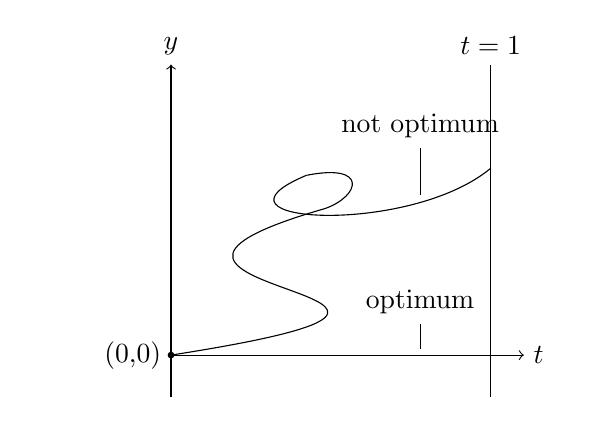
\begin{tikzpicture}[x=0.75pt,y=0.75pt,yscale=-1,xscale=1]
%uncomment if require: \path (0,319); %set diagram left start at 0, and has height of 319

%Curve Lines [id:da9395362233161386] 
\draw    (0,290) .. controls (196.2,259.4) and (-68.8,260.4) .. (74.2,219.4) ;
%Curve Lines [id:da4305029991293019] 
\draw    (65.2,203.4) .. controls (10.2,226.4) and (114.5,232.9) .. (154,200) ;
%Curve Lines [id:da9651462462408447] 
\draw    (65.2,203.4) .. controls (95.2,197.4) and (91.2,213.4) .. (74.2,219.4) ;
%Straight Lines [id:da18765309009648878] 
\draw[->]    (0,290) -- (170,290) node [right] {$t$} ;
\draw    (154,310) -- (154,150) node [above] {$t=1$} ;
\draw[->]    (0,310) -- (0,150) node [above] {$y$} ;
 
\filldraw [black]  (0,290) circle (1pt) node [left] {(0,0)}  ;

\draw (120,287) -- (120,275) node [above] {optimum} ; 
\draw (120,213) -- (120,190) node [above] {not optimum} ; 
\end{tikzpicture}
\caption{The shortest distance} %最终文档中希望显示的图片标题
\label{Fig11.1} %用于文内引用的标签
\end{figure}

Consider the path of minimum length between the points (0,0) and (1,0) in the plane; see Figure \ref{Fig11.1}. Call the horizontal coordinate $t$ and the vertical coordinate $y$. It is clear that any path which loops or winds cannot be of minimum length, because we can simply omit the loop or an S-shape to get a shorter one. We can therefore restrict discussion to the case where $y$ is a single-valued function of $t$. The distance between the adjacent points $(t,y)$ and $(t + dt,y + dy)$ is $[(dt)^2 + (dy)^2]^{1/2}$. Let $dy/dt = z$, the control variable. Then we are to maximize
\begin{equation} \label{equa11.23}
 - \int_0^1 [1+z(t)^2]^{1/2} dt
\end{equation}
subject to 
\begin{equation} \label{equa11.24}
  \dot{y}(t) = z(t)
\end{equation}
and $y(0)=y(1)=0$.

To use the Maximum Principle, define the Hamiltonian
\begin{equation} \label{equa11.25}
  H = -(1+z^2)^{1/2} + \pi z
\end{equation}
The first-order condition for $z$ to maximize this is
\begin{equation*}
  -(1+z^2)^{-1/2}z + \pi = 0
\end{equation*}
which simplifies to
\begin{equation} \label{equa11.26}
   z = \pi / (1-\pi^2)^{1/2}
\end{equation}
Then the maximized Hamiltonian is 
\begin{equation} \label{equa11.27}
  H^* = -(1-\pi^2)^{1/2}
\end{equation}

Now the two differential equations are
\begin{equation} \label{equa11.28}
  \dot{y} = \partial H^* / \partial \pi = \pi / (1-\pi^2)^{1/2}
\end{equation}
and
\begin{equation} \label{equa11.29}
  \dot{\pi} = - \partial H^* / \partial y = 0
\end{equation}
Thus $\pi$ is constant along the optimal path, and then so is $z$. But the only constant $z$ that will keep $y(1) = y(0)$ is zero. Thus the shortest path is the horizontal straight line joining (0,0) and (1,0).

We can apply Dynamic Programming and consider a somewhat more general problem, namely finding the shortest line joining (0,0) to the liner $t= 1$. First we consider the subproblem joining (0,0) to the general point $(T, y)$ with $T > 0$ but $y$ unconstrained. The theory above continues to apply, and we see that the straight line $y(t) = ty/ T $ does the job. Now it remains to choose $y$ optimally. The transversality condition for that is $\pi(T) = 0$. Since $\pi$ is constant along the optimal path, it must be zero everywhere. Then $z$ must be zero, and therefore $y(T) = 0$ is optimal. In other words, the shortest path from a point to a line is the straight line from the point and perpendicular to the given line.

\section*{Exercises}

\subsubsection*{\textit{Exercise 11.1: Search}}

Consider a variant of the search problem of Example 11.1. Suppose that the searcher can return to old jobs that he had rejected. So at any time, the state variable $x$ is the best offer he had observed up to that point. If he rejects this, searches and observes $y$, then next period he will start with the better of $x$ and $y$. Thus instead of (\ref{equa11.14}) we have
\begin{equation*}
  V_n(x) = \max \ \{ x(1-\delta^n)/(1-\delta), \ \delta E[V_{n-1}(\max (x,y)) ] \  \}
\end{equation*}
Show that there is a reservation wage $x_n^*$, and that the sequence of reservation wages is increasing in $n$. Write down the Bellman Equation as $n$ goes to infinity, and characterize its $x^*$. Note that
\begin{equation*}
\begin{array}{rl}
 E[V(\max(x,y))] = & \int_0^x V(x) \phi(y) dy + \int_x^\infty V(y) \phi(y) dy \\
                 = & V(x) \Phi(x) + \int_x^\infty V(y) \phi(y) dy 
\end{array}
\end{equation*}

\subsubsection*{\textit{Exercise 11.2: Intensity of Research Effort}}

The research and development needed for a new product consists of completion of a number of stages. Think of these as a continuum of length $L$. If $x(t)$ stages are completed at time $t$, and flow cost $c(t)$ is incurred on the R\&D program at this time, then the completion process evolves according to the differential equation
\begin{equation*}
  \dot{x} = f(x)
\end{equation*}
When all $L$ stages are completed, a reward $R$ accrues. If this occurs at time $T$, and $r>0$ is the rate of interest, the net present value of the program is 
\begin{equation*}
  R e^{-rT} - \int_0^T c(t) e^{-rt}dt
\end{equation*}
The aim is to choose the completion time $T$ and the profile of costs $c(t)$ over $[0,T]$ to maximize this.

Define $V(x)$ to be the value function for the corresponding problem that starts with $x$ stages completed. Applying Bellman's Principle over an initial small time interval $dt$, we have
\begin{equation*}
 V(x) = \mathop{\max}\limits_c \ \{ -cdt + V[x+ f(c)dt]e^{-rdt} \}
\end{equation*}
Expanding the right-hand side in a Taylor series as in the derivation of (\ref{equa11.5}), convert this into
\begin{equation} \label{equa11.30}
 r V(x) = \mathop{\max}\limits_c \ [ V^\prime(x)f(c) - c ]
\end{equation}

For the case $f(c) = c^\alpha$, with $0<\alpha <1$, the maximization in (\ref{equa11.30}) can be performed explicitly. Show that it yields
\begin{equation*}
   V^\prime(x) = \beta V(x)^{1-\alpha}
\end{equation*}
where $\beta$ is a known constant that depends on $r$ and $\alpha$. Solve this to show that
\begin{equation} \label{equa11.31}
  V(x)^\alpha = R^\alpha + \alpha \beta (x-L)
\end{equation}

Deduce that $V$ is a convex function, and therefore that the optimal intensity of research effort starts at a low level, and rises as more stages get completed. (Try offering this as an excuse for procrastination to your teachers, bosses etc.)

If $L$ is large enough, it may be optimal not to embark on this program of research at all. Find the limit on $L$. Solve the whole problem using the Maximum Principle.

How can the problem be modified to allow for uncertainty in the progress of research?









%\chapter*{Appendix: The Kuhn-Tucker Theorem}
% \markboth{Appendix: The Kuhn-Tucker Theorem}{}

\begin{appendices}
\chapter{The Kuhn-Tucker Theorem} 
  
%\setcounter{equation}{0}
%\renewcommand\theequation{A.\arabic{equation}}

%\setcounter{figure}{0}
%\renewcommand{\thefigure}{A.\arabic{figure}}

The purpose of the Appendix is to offer the sketch of a rigorous proof of the Kuhn-Tucker Theorem, which is the most general theorem on first-order necessary conditions for maximization subject to non-negativity and inequality constraints. Notice the word `sketch': this is not a detailed proof, but each heuristic argument in the sketch can easily be converted into a rigorous one. This should suffice for most readers. I begin by recapitulating the statement of the theorem from Chapter 3:

\textit{Kuhn-Tucker Theorem:} Suppose $x$ is an $n$-dimensional vector, $c$ an $m$-dimensional vector, $F$ a function taking scalar values, $G$ a
function taking $m$-dimensional vector values. Define
\begin{equation*} \tag{3.4}
 L(x, \lambda) = F(x) + \lambda [c-G(x)]
\end{equation*}
where $\lambda$ is an $m$-dimensional row vector. Suppose $\bar{x}$ maximizes $F(x)$ subject to $G(x) \leq c$ and $x \geq 0$, and the constraint qualification holds, namely the submatrix of $G_x(\bar{x})$ formed by taking those rows $i$ for which $G^i(\bar{x}) = c$, has the maximum possible rank. Then there is a value of $\lambda$ such that
\begin{equation*} \tag{3.7}
L_x(\bar{x}, \lambda) \leq 0, \ \bar{x} \geq 0, \quad \mbox{with complementary slackness}
\end{equation*}
and
\begin{equation*} \tag{3.10}
L_\lambda(\bar{x}, \lambda) \geq 0,  \ \lambda \geq 0, \quad \mbox{with complementary slackness}
\end{equation*}

Before we begin the proof, we can simplify the notation. The non-negativity constraints can be expressed as $—x_j \leq 0 $ for $j = 1,2, \dots n$. Thus we can subsume them into the general inequality constraints, whose number $m$ is increased accordingly. We can also choose the labels on the component functions $G^i$ such that constraints $1, 2, \dots k$ are binding, and $k + 1, \dots m$ are slack, or
\begin{equation} \label{equaA.1}
G^i(\bar{x}) \left\{  \begin{array}{ll}
= c_i & \mbox{for} \  i=1,2,\dots k \\
< c_i & \mbox{for} \ i = k+1, \dots m 
\end{array}
\right.
\end{equation}

Since $\bar{x}$ is a maximizer (local or global) of $F(x)$ subject to $G(x) \leq c$, there is no neighboring $x$ such that 
\begin{equation} \label{equaA.2}
 G^i(x) \leq G^i(\bar{x}) = c_i  \quad \mbox{for} \ i=1,2,\dots k
\end{equation}
and
\begin{equation} \label{equaA.3}
F(x) > F(\bar{x})
\end{equation}
Note that we do not need any restrictions arising from the constraints $k+1, \dots m$; since the constraints hold as strict inequalities at $\bar{x}$, by continuity they will go on holding for $x$ sufficiently near $\bar{x}$.

Now write $x=\bar{x} +dx$ where $dx$ is infinitesimal. Then we want to replace (\ref{equaA.2}) and (\ref{equaA.3}) by the first-order Taylor approximations:
\begin{equation} \label{equaA.4}
 G_x^i(\bar{x}) dx \leq 0  \quad \mbox{for} \ i=1,2,\dots k
\end{equation}
and
\begin{equation} \label{equaA.5}
  F_x(\bar{x}) dx > 0
\end{equation}

This is valid provided the $k \times n$ matrix $G_x(\bar{x})$ formed by stacking the $k$ rows $G_x^i(\bar{x})$ has rank $k$. If it has a smaller rank, it has too large a null space, that is, too many vectors $dx$ yield zero when multiplied by this matrix. Then many more $dx$ satisfy the linear approximation (\ref{equaA.4}) than do $\bar{x} +dx$ satisfy the true constraints (\ref{equaA.2}). As a result, the first-order conditions can fail even though $\bar{x}$ is optimum.

I shall illustrate this using an example with two variables and two constraints. Suppose the objective function is 
\begin{equation*}
F(x_1, x_2) = x_1
\end{equation*}
and the constraints are
\begin{equation*}
 x_2 \geq x_1^3, \quad \mbox{or} \quad G^1(x_1, x_2) \equiv x_1^3 - x_2 \leq 0
\end{equation*}
\begin{equation*}
 x_2 \leq - x_1^3, \quad \mbox{or} \quad G^2(x_1, x_2) \equiv x_2 + x_1^3 \leq 0
\end{equation*}

\begin{figure}[!htb] %H为当前位置,!htb为忽略美学标准,htbp为浮动图形
\centering %图片居中
%\includegraphics[width=0.8\textwidth]{./Fig3.1.png} %插入图片,[]中设置图片大小,{}中是图片文件名
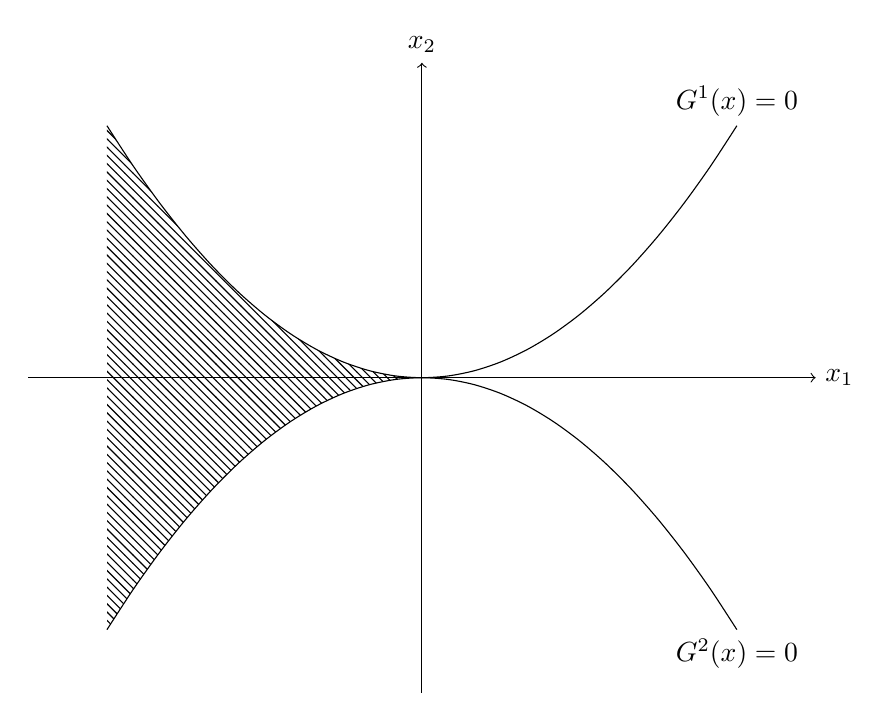
\begin{tikzpicture}[scale=1.0  ]
    % 绘制坐标轴
    \draw[->] (-5,0) -- (5,0) node[right] {$x_1$};
    \draw[->] (0,-4) -- (0,4) node[above] {$x_2$};
   % \draw[black] (0,0) node[below left] {$O$};

\fill[pattern=north west lines] plot[smooth,samples=100,domain=-4:0] (\x,{0.2*\x*\x}) -- plot[smooth,samples=100,domain=0:-4] (\x,{-0.2*\x*\x});
\draw[domain=-4:4,smooth,variable=\x, black] plot ({\x},{0.2* \x * \x  }) ;
\draw[domain=-4:4,smooth,variable=\x, black] plot ({\x},{-0.2* \x * \x  }) ;
 
\draw (4,3.2) node [above] {$G^1(x)=0$}; 
\draw (4,-3.2) node [below] {$G^2(x)=0$}; 
\end{tikzpicture}
\caption{Failure of the constraint qualification} %最终文档中希望显示的图片标题
\label{FigA.1} %用于文内引用的标签
\end{figure}
Figure \ref{FigA.1} shows the feasible set as the shaded area, and then it is clear that (0,0) solves the constrained maximization problem.

At this point both constraints bind $(k=2)$, and the vectors of derivatives of the constraints are
\begin{equation*}
G_x^1(0,0) = (0,-1) \quad \mbox{and} \quad G_x^2(0,0) = (0,1)
\end{equation*}
The rows are linearly dependent, and the rank of the matrix of derivatives is 1, which is <$k$. The linear approximation (\ref{equaA.4}) becomes
\begin{equation*}
 -dx_2 \leq 0 \quad \mbox{and} \quad dx_2 \leq 0, \quad \mbox{that is,} \quad dx_2=0
\end{equation*}
which is the whole horizontal axis. Points to the right of the origin are not in fact a linear approximation to the feasible set, but they appear as feasible deviations in the linear approximation to the functions.

Now we also see the sense of the remark made earlier in the context of linear programming (Example 7.1) that no constraint qualification was needed there. When the constraints are already linear, there is no need to find linear approximations to them, so the issue does not arise.
\begin{figure}[!htb] %H为当前位置,!htb为忽略美学标准,htbp为浮动图形
\centering %图片居中
%\includegraphics[width=0.8\textwidth]{./Fig3.1.png} %插入图片,[]中设置图片大小,{}中是图片文件名
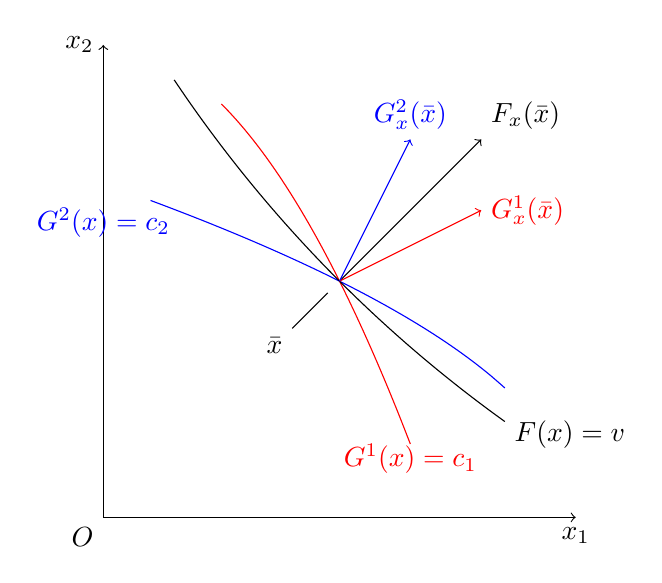
\begin{tikzpicture}[scale=3  ]
    % 绘制坐标轴
    \draw[->] (0,0) -- (2,0) node[below] {$x_1$};
    \draw[->] (0,0) -- (0,2) node[left] {$x_2$};
    \draw[black] (0,0) node[below left] {$O$};

\draw[domain=0.5:1.3,smooth,variable=\x, red] plot ({\x},{2 -  \x * \x  }) ;
\draw[domain=0.2:1.7,smooth,variable=\x, blue] plot ({\x},{ sqrt(2 -  \x)    }) ;
\draw[domain=0.3:1.7,smooth,variable=\x, black] plot ({\x},{ 5- sqrt(32 - (\x-5)*(\x-5) )  }) ;

\draw[->] (1,1) -- (1.6,1.6) node [above right] {$F_x(\bar{x})$} ;
\draw[->, red] (1,1) -- (1.6,1.3) node [right] {$G_x^1(\bar{x})$} ;
\draw[->, blue] (1,1) -- (1.3,1.6) node [above] {$G_x^2(\bar{x})$} ;


\draw[black] (0.95,0.95) -- (0.8,0.8) node[below left] {$\bar{x}$} ;
\draw[red] (1.3,0.35) node[below] {$G^1(x)=c_1$} ;
\draw[blue] (0,1.35) node[below] {$G^2(x)=c_2$} ;
\draw[black] (1.7,0.35) node[right] {$F(x)=v$} ;
\end{tikzpicture}
\caption{The Kuhn-Tucker Theorem} %最终文档中希望显示的图片标题
\label{FigA.2} %用于文内引用的标签
\end{figure}
Let us proceed with the assumption (the Constraint Qualification) that the rank of $G_x(\bar{x})$ equals $k$. Figure \ref{FigA.2} shows the situation. It is drawn so that all functions are increasing in $x$, but that is only to conform to the economic intuition; other configurations make no difference. The feasible region, and the upper contour set of $F(x)$ for its optimal value, are both shown by hatch-marks on their boundaries. The vector of derivatives of each of the functions is also shown; each is normal (perpendicular) to the contour curve of the corresponding function.

When $\bar{x}$ is optimum, the feasible region and the upper contour set of the objective function should not intersect. Assuming validity of the constraint qualification, their linear approximations defined by the deviations in (\ref{equaA.4}) and (\ref{equaA.5}) should not intersect either. For this to be true, the vector of derivatives $F_x(\bar{x})$ should lie in the cone formed by the vectors $G_x^i(\bar{x})$ of the derivatives of the constraint functions. This is more easily seen from the equivalent statement in the opposite direction (contrapositive) from the figure: if $F_x(\bar{x})$ were to lie outside this cone, the contour of $F$ through $\bar{x}$ would cut into the feasible region, so a neighboring feasible point with a higher value could be found, and $\bar{x}$ could not be optimal.

Points in a finite cone are non-negative linear combinations of the vectors that define the cone. Therefore there are non—negative numbers $\lambda_1, \lambda_2, \dots \lambda_k $ such that
\begin{equation} \label{equaA.6}
 F_x(\bar{x}) = \sum\limits_{i=1}^k \lambda_i G_x^i(\bar{x})
\end{equation}
It is harmless to extend the range of summation to $m$ by defining $\lambda_{k+1}, \dots, \lambda_m$ all equal to zero. The extended (\ref{equaA.6}) is just the condition $L_x( \bar{x}, \lambda) = 0$ to which (\ref{equa3.7}) reduces when there are no non-negativity constraints (remember they are subsumed into the inequality constraints and so do not have a separate role). The complementary slackness condition (\ref{equa3.10}) is fulfilled because of the way the $\lambda_i$ are defined for the slack constraints. This completes the sketch of the proof.

\end{appendices}








\backmatter
% bibliography, glossary and index would go here.

\end{document}